\chapter{BLOSTE}
\label{ch:bloste}

Tras presentar \gls{d2e} (Capítulo~\ref{ch:den2ne}) y exponer una propuesta que extiende \gls{d2e} hacia un servicio de optimización y reconfiguración proactiva para \glspl{sg} (Capítulo~\ref{ch:fault_sg}), se avanzó en una colaboración con el Departamento de Electrónica de la UAH para adaptar y versionar \gls{d2e} específicamente al dominio de las redes inteligentes de distribución en el marco del \gls{ei}. Esta colaboración permitió un ajuste fino (\textit{fine-tuning}) de los criterios de optimización y la incorporación de conocimiento experto en electrónica de potencia para hacer la solución más adecuada al entorno real de distribución eléctrica.\\
\\
De esta colaboración nace \gls{blo}, un marco reconfigurable que aprovecha topologías malladas configurables como soporte para una distribución de energía más eficiente y resiliente. \gls{blo} crea una superposición lógica dinámica sobre la infraestructura física de la red, habilitando a cada nodo para calcular múltiples rutas hacia los nodos raíz y seleccionar de forma autónoma la ruta óptima según cuatro criterios de optimización parametrizables. Este esquema facilita el equilibrio energético local, promueve la autosuficiencia entre prosumidores vecinos y reduce la dependencia del suministro central, con los beneficios esperados de menor pérdida energética, menor desequilibrio y postergación de costosas ampliaciones de infraestructura.\\
\\
El capítulo describe el diseño conceptual de \gls{blo}, los criterios de selección y reconfiguración, las implicaciones prácticas reales y los resultados experimentales conseguidos sobre topologías del \gls{ieee} ampliamente conocidas en el mundo de las \gls{sg}. Finalmente, parte de este trabajo ha dado lugar a una publicación enviada a una revista de alto impacto (Carrascal \textit{et al.}~\cite{carrascal2025dynamic}).

\section{Introducción}

Como se ha podido estudiar en el Estado del Arte (Sección~\ref{subsec:sg}), la transición energética global está tendiendo hacia sistemas eléctricos más sostenibles, resilientes y eficientes que exigen replantear las arquitecturas de distribución de energía. El incentivo de la integración masiva de generadores renovables con la Directiva 2018/2001/UE sobre energías renovables~\cite{euREDII},  materializada en España a través del Real Decreto 244/2019~\cite{rd2442019}, y la descentralización de la producción han incrementado la complejidad operativa y de control de las redes de distribución, complicando tareas de planificación, protección y coordinación~\cite{GADELHA2024110581}.\\  
\\
En respuesta a estos cambios, las topologías radiales tradicionales están dando paso a configuraciones más malladas. Las redes malladas ofrecen mayor flexibilidad operativa al habilitar múltiples trayectorias para el flujo de potencia, lo que reduce la dependencia de rutas únicas, mejora la continuidad del suministro y facilita la integración de recursos distribuidos (\glspl{der}). Sin embargo, este beneficio conlleva retos: los flujos de potencia se vuelven más dinámicos y menos predecibles, aumentando las exigencias de control, la complejidad de la protección y la necesidad de respuestas locales rápidas. Para afrontar estos retos son necesarias arquitecturas con inteligencia distribuida y capacidad de reconfiguración en tiempo real, lo que motiva la adopción de elementos como los \glspl{er}~\cite{Zhou24} y paradigmas tipo \gls{ei}~\cite{Xu11}.\\
\\
Una tecnología habilitadora fundamental para el \gls{ei} es el \gls{er}~\cite{Zhou24}. Estos dispositivos, basados en electrónica de potencia de alto rendimiento, permiten un control programable y dinámico de los flujos en redes de distribución: regulan variables eléctricas (tensión, corriente, frecuencia) y permiten el enrutamiento selectivo de potencia entre nodos~\cite{Zhu25}. Su funcionamiento es análogo al de los routers en redes de datos y supone un cambio de paradigma en la gestión de la electricidad a nivel de distribución. La integración de \glspl{er} habilita la arquitectura conocida como \gls{prg}, en la que los \glspl{er} actúan como nodos inteligentes que interconectan activos heterogéneos (generación convencional y renovable, almacenamiento, cargas), permitiendo la optimización dinámica del flujo de energía según demanda, oferta, precios de mercado y restricciones operativas~\cite{Liu18}.\\
\\
A pesar del progreso en la literatura sobre encaminamiento energético y arquitecturas para el \gls{ei}, persisten limitaciones relevantes: (i) muchas soluciones son estáticas o centralizadas, lo que restringe su escalabilidad y adaptabilidad; (ii) hay escasez de enfoques que exploten topologías multi-raíz o malladas con decisiones autónomas a nivel de nodo; (iii) falta consenso sobre criterios de selección de rutas que equilibren pérdidas, balance local y resiliencia; y (iv) la integración de tecnologías emergentes (p. ej., blockchain para validación transaccional o \gls{ai} para encaminamiento predictivo) está aún poco explorada. Estos vacíos subrayan la necesidad de marcos de encaminamiento flexibles, distribuidos y en tiempo real capaces de operar en entornos heterogéneos y dinámicos.\\
\\
En este contexto presentamos \gls{blo}, un marco de encaminamiento dinámico diseñado para abordar los retos de las redes de distribución de próxima generación. \gls{blo} construye una superposición lógica sobre la infraestructura física mallada mediante procedimientos de etiquetado jerárquico que permiten a cada nodo aprender múltiples rutas hacia uno o varios nodos raíz. A diferencia de enfoques centralizados, \gls{blo} facilita la toma de decisiones autónoma en el propio nodo basada en información local y en criterios de encaminamiento configurables. Su diseño prioriza la resiliencia y la eficiencia: los nodos pueden seleccionar rutas según objetivos operativos distintos (minimizar saltos, pérdidas, o equilibrar potencia local), y el sistema incorpora mecanismos de refresco y estrategias de respaldo para adaptarse a degradaciones de enlace o cambios topológicos. Las principales contribuciones de este capítulo son:

\begin{itemize}
    \item \textbf{Formación dinámica de topologías lógicas.} Método para generar, desde uno o varios nodos raíz, topologías lógicas jerarquizadas sobre una red física mallada mediante etiquetado, facilitando el aprendizaje de múltiples rutas por nodo.
    
    \item \textbf{Criterios de encaminamiento configurables.} Implementación de cuatro criterios ajustables (mínimos saltos, minimización de pérdidas, balance local a cero y balance local ponderado por pérdidas) que cada nodo puede emplear de forma autónoma para seleccionar su ruta activa.
    
    \item \textbf{Resiliencia operativa.} Mecanismos periódicos de refresco y políticas de conmutación que permiten recomputar rutas y mantener servicio ante degradaciones o fallos, sin depender exclusivamente de control central.
    
    \item \textbf{Algoritmo eficiente de balance de potencia.} Procedimiento iterativo de reparto de carga que converge hacia estados globalmente equilibrados minimizando pérdidas de transmisión.
    
    \item \textbf{Evaluación exhaustiva.} Validación experimental sobre las topologías \gls{ieee} 123-node y 34-node test feeder,  mediante un amplio conjunto de simulaciones (escenarios ideales, con pérdidas y con pérdidas+capacidad limitada), que demuestra la capacidad de \gls{blo} para mejorar tiempos de convergencia, balance energético y adaptabilidad, destacando especialmente el criterio de balance local a cero.
    
\end{itemize}

En las secciones siguientes se presenta con detalle la arquitectura de \gls{blo}, los algoritmos de etiquetado y selección de rutas, el procedimiento de balance energético y los resultados de la evaluación, incluyendo un análisis computacional frente a estrategias alternativas y una discusión sobre su aplicabilidad práctica en \glspl{prg}.

\section{Enfoque jerárquico de redistribución de energía basado en árboles}
\label{sec:distribution}

Como se ha destacado previamente, las redes de distribución eléctrica tienden hacia un modelo más hiperconectado o en malla para mejorar su rendimiento y eficiencia y aprovechar mejor la generación distribuida asociada a las energías renovables~\cite{kafle2016towards}. Este cambio hacia arquitecturas malladas ha sido respaldado por diversos estudios que subrayan las ventajas de la operación en malla para facilitar la integración de generadores renovables variables~\cite{cruz2018meshed,cruz2018prospects}. Por ejemplo, algunos autores destacan ya el potencial de los sistemas de distribución eléctrica mallados para acoger generación renovable variable a gran escala~\cite{cruz2018prospects}. Asimismo, se han propuesto arquitecturas en malla basadas en LoRa para la automatización de redes rurales de distribución eléctrica, demostrando la aplicabilidad de las estructuras malladas más allá de entornos urbanos~\cite{prade2020lora}. La motivación detrás de la transición hacia una red eléctrica hiperconectada radica en su capacidad para gestionar de forma eficaz la generación descentralizada procedente de fuentes renovables, optimizar la distribución de la energía y aumentar la resiliencia del sistema en su conjunto~\cite{kafle2016towards}. Modelar la red de distribución como una estructura mallada se alinea con este propósito, ya que permite flujos de energía más dinámicos y eficientes~\cite{cruz2018meshed}. Al conceptualizar la red mallada como un grafo, es posible visualizar sus interconexiones y los distintos caminos de flujo, lo que facilita la comprensión de su dinámica operativa~\cite{zhou2021mesh}.\\
\\
Para ilustrar este proceso, introducimos la Figura~\ref{fig:bloste_01}, que muestra cómo puede representarse una red de distribución de energía hiperconectada como un grafo. El proceso comienza con la caracterización de la red de distribución: identificación de fuentes de generación, consumidores y las líneas de transmisión que los conectan (Figura~\ref{fig:bloste_01}a). Esta información se emplea para construir un grafo en el que generadores y consumidores se representan como nodos y las líneas eléctricas como enlaces (Figura~\ref{fig:bloste_01}b). Además, la naturaleza heterogénea de los agentes, generación, industria, transporte, residencial, almacenamiento, etc.,  implica perfiles de consumo variados que cambian dinámicamente según las condiciones ambientales (clima, horarios laborales, festivos, etc.), dando lugar a una red de potencia con múltiples fuentes y consumos variables en el tiempo, donde es necesario optimizar el equilibrio de las cargas (Figura~\ref{fig:bloste_01}c).

\begin{figure}[ht!]
    \centering
    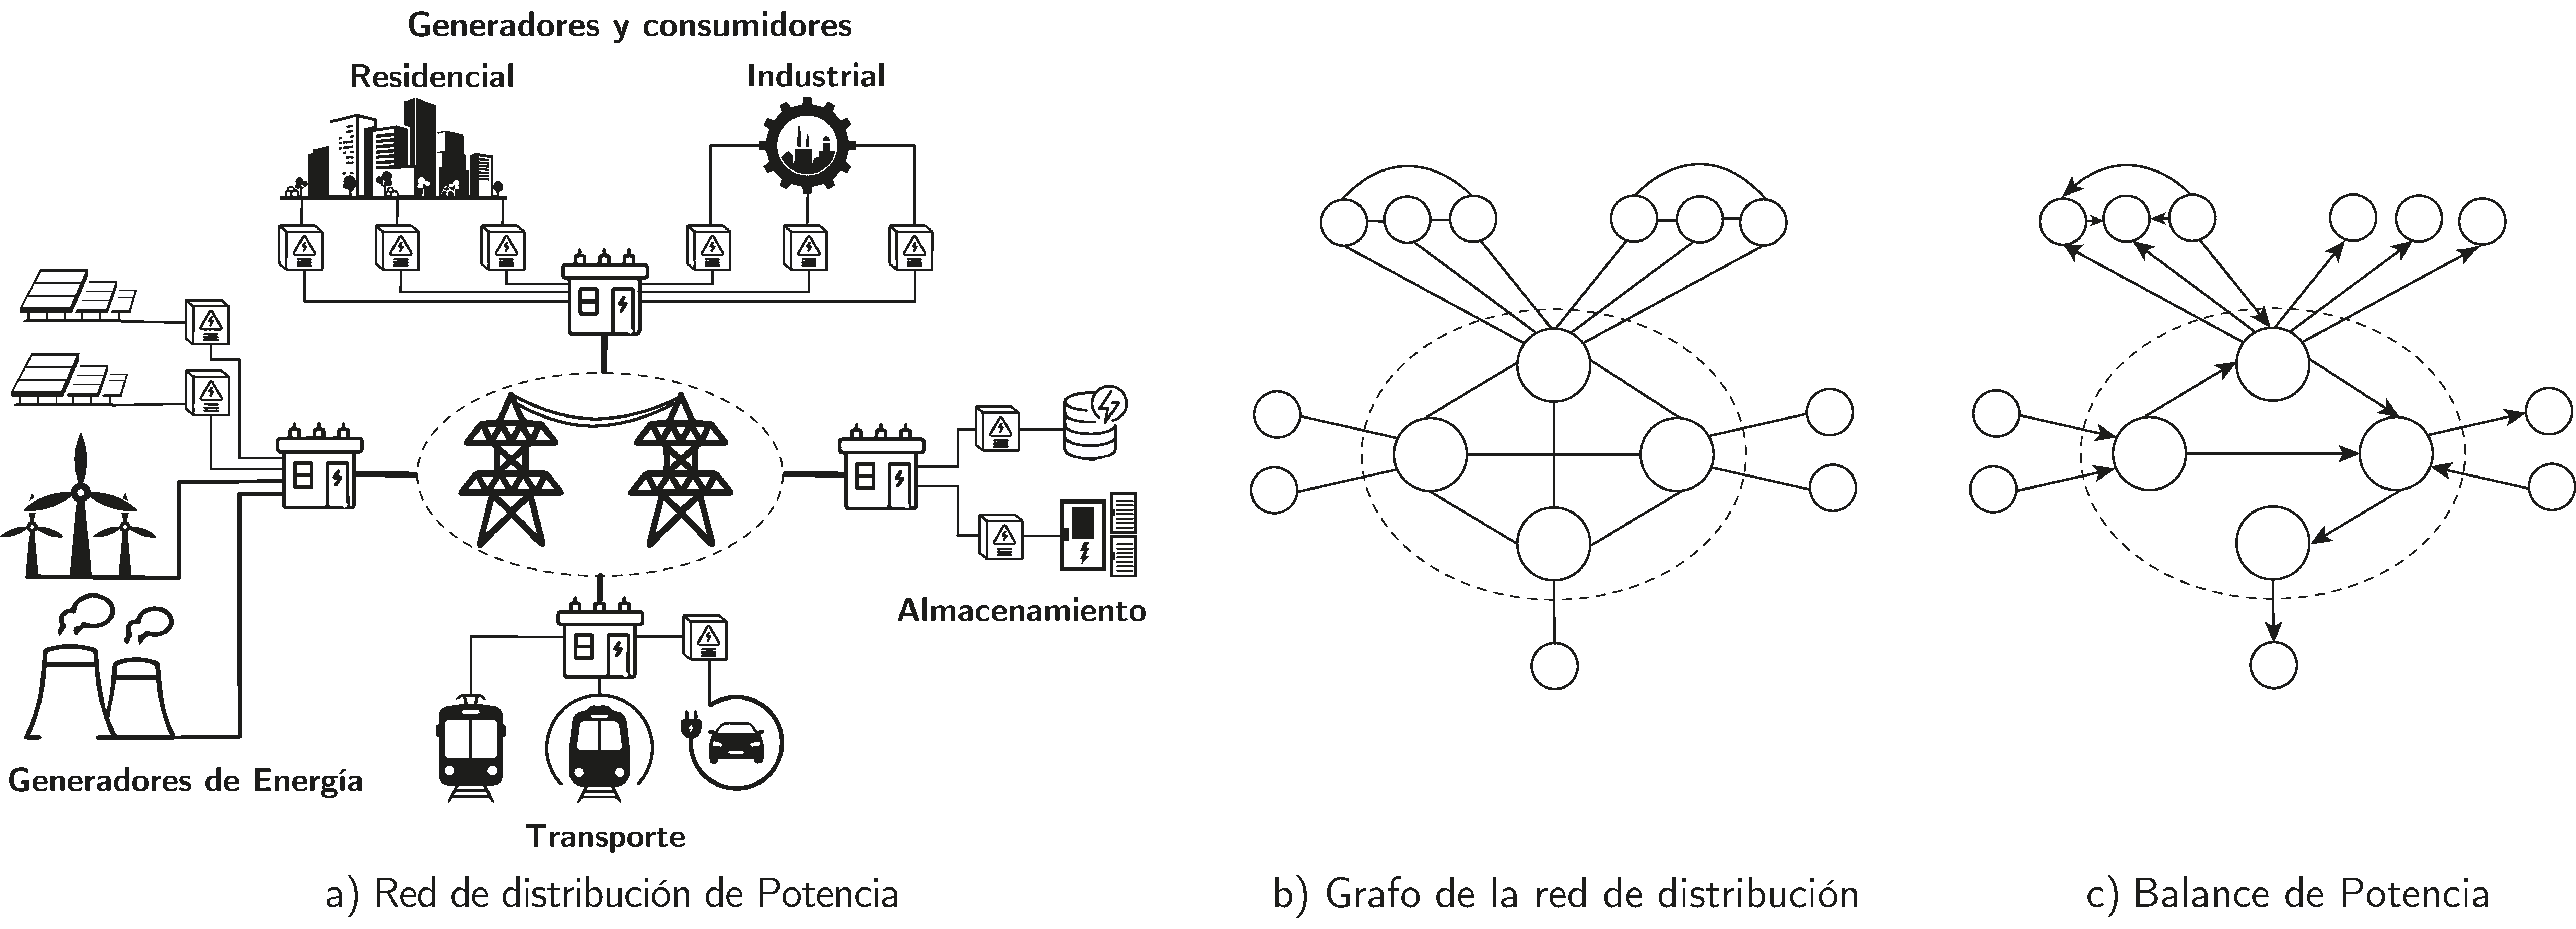
\includegraphics[width=\textwidth]{fig/07_bloste/bloste_01.pdf}
    \caption{Ejemplo de distribución de potencia.}
    \label{fig:bloste_01}
\end{figure}

\subsection{Construcción de la topología lógica}
\label{subsec:logical-topo}

Como hemos visto a lo largo de la Tesis, la modelización de la topología lógica puede expresarse en forma matemática: dado un grafo \( G = (\mathcal{N}, \mathcal{L}) \), que representa la topología completa, donde \( \mathcal{N} \) es un conjunto de \( N \) nodos y \( \mathcal{L} \) un conjunto de \( L \) enlaces tal que \( \mathcal{L} \subseteq \{\{i,j\} \: | \: i,j \in \mathcal{N} \: \forall \: i \neq j\} \). En función del balance de potencia de la red de distribución eléctrica en un instante dado, puede definirse un subgrafo \(G'\) a partir de \(G\) que toma parte de los elementos dependiendo de la oferta y la demanda de energía en los distintos nodos, denotado como \( G' = (\mathcal{N}', \mathcal{L}') \), donde \( \mathcal{N}' \subseteq \mathcal{N} \) y \( \mathcal{L}' \subseteq \mathcal{L} \). De esta manera, se pueden obtener diferentes topologías lógicas en distintos momentos en función de las condiciones energéticas, pudiendo optimizar de esta forma la topología final, prescindiendo de enlaces innecesarios para la distribución eléctrica.


\begin{figure}[ht!]
    \centering
    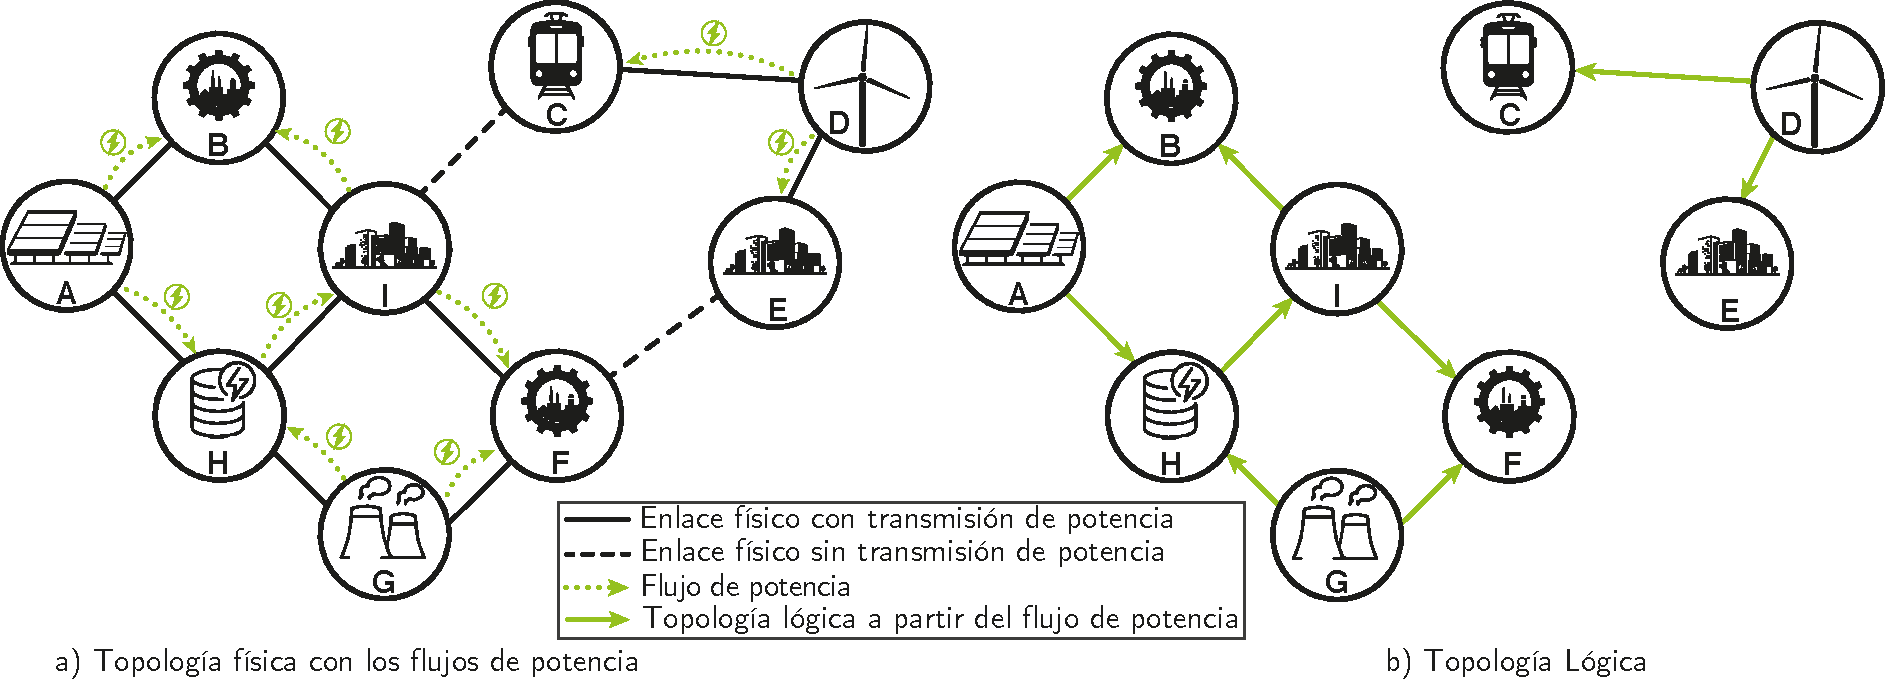
\includegraphics[width=\textwidth]{fig/07_bloste/bloste_02.pdf}
    \caption{Establecimiento de la topología lógica.}
    \label{fig:bloste_02}
\end{figure}

La Figura~\ref{fig:bloste_02} proporciona un ejemplo de cómo puede derivarse una topología lógica a partir de un grafo físico. Se divide en dos secciones: la sección izquierda (Figura~\ref{fig:bloste_02}a) ilustra la topología de la red de distribución física, grafo \(G\), mientras que la sección derecha (Figura~\ref{fig:bloste_02}b) muestra la topología lógica \(G'\) derivada del grafo físico \(G\), considerando las demandas y excedentes de potencia de la red de distribución. Más específicamente, este ejemplo contiene una topología con 9 nodos identificados de manera única, etiquetados de la \textit{A} a la \textit{I}, los cuales están conectados mediante líneas de transmisión eléctrica. Las líneas de transmisión se representan como líneas continuas o discontinuas, indicando si están transportando energía de forma activa o si se encuentran inactivas, respectivamente. Por ejemplo, el enlace que conecta los nodos \textit{I} y \textit{C} no transporta energía, por lo que se representa con una línea discontinua, mientras que el enlace entre \textit{C} y \textit{D} sí transporta energía y, por tanto, se representa con una línea continua. \\
\\
Los nodos de la red se categorizan según su función como nodos demandantes, con excedentes o mixtos, mientras que el flujo de energía entre nodos se representa mediante una flecha verde punteada. Por ejemplo, el nodo \textit{A} representa un generador solar, por lo que es un nodo con excedentes que suministra energía a los nodos \textit{B} (un nodo demandante), un parque industrial que demanda energía, y \textit{H}, un nodo de almacenamiento que tanto demanda como suministra energía a otros nodos (un nodo mixto). El resto de los nodos contribuyen de manera análoga al balance energético de la red según su rol.\\
\\
Toda la información anteriormente descrita se encuentra en la Figura~\ref{fig:bloste_02}a, a partir de la cual pueden derivarse múltiples topologías lógicas dependiendo del balance energético de la red y de las estrategias de distribución adoptadas. Las dos topologías lógicas resultantes de este ejemplo se ilustran en la Figura~\ref{fig:bloste_02}b. Éstas representan dos islas energéticas aisladas que optimizan el balance de energía, garantizando que la demanda sea cubierta y minimizando las pérdidas debidas a inserción y reflexión en enlaces inactivos de la red de distribución. Como se explicó previamente, esta topología lógica constituye la representación de la red en un instante concreto. En consecuencia, dicha topología lógica no es estática, es decir, cambia en el tiempo en función de las ofertas y demandadas de la red.\\
\\
Por lo tanto, existe una clara necesidad de un mecanismo específico que permita calcular y gestionar topologías lógicas de manera dinámica, con el fin de habilitar una distribución eficiente de la energía a lo largo de la red bajo condiciones variables. Para abordar esta necesidad, en este trabajo se introduce un mecanismo que explora y caracteriza sistemáticamente la red de distribución eléctrica mediante un procedimiento de etiquetado jerárquico basándonos en las lecciones aprendidas de \gls{d2e}. Este enfoque sienta las bases para la construcción de topologías lógicas adaptadas a objetivos de optimización concretos en \gls{sg}, tales como minimizar las pérdidas de energía o maximizar el balance energético. Los detalles del proceso de exploración y etiquetado, que constituyen el núcleo de nuestra propuesta, se describen en las siguientes secciones.


\subsubsection{Procedimiento de etiquetado jerárquico basado en un árbol}
\label{subsec:tree}

Esta sección describe en detalle un procedimiento de distribución de etiquetas para construir un árbol jerárquico a partir de un nodo seleccionado de una topología, denominado \textit{nodo raíz}. En teoría de grafos (Ver Sección~\ref{subsubsec:teminologia_grafos}), un árbol es un tipo especial de grafo conexo que es acíclico. Esto significa que no contiene ciclos y que cada par de nodos en el grafo está conectado por un único camino. Además, el nodo raíz es el nodo superior del cual se derivan el resto. Cada nodo en el árbol tiene exactamente un nodo padre y cero o múltiples nodos hijos, mientras que el nodo raíz no tiene padre y solo posee nodos hijos. Esto establece una jerarquía que estructura el árbol en múltiples niveles.\\
\\
Para construir una topología lógica a partir de una topología física, nuestra propuesta establece un procedimiento de etiquetado jerárquico desde un nodo (el nodo raíz) con el objetivo de establecer relaciones estructurales lógicas entre los nodos de la topología que permitan satisfacer la demanda y la producción de energía. Este nodo raíz, desde el cual comienza el procedimiento de etiquetado jerárquico, puede ser un punto de generación, transformación o distribución de energía, entre otros, dependiendo de las necesidades de la red. Cada nodo de la red debe contar con un identificador único (ID), ya que este ID se difunde de manera controlada a través de la red para recopilar información y establecer la jerarquía de la topología. Este ID puede ser un número, una letra o una cadena alfanumérica, siempre que sea único para cada nodo.\\
\\
Para explicar mejor el procedimiento, el proceso de difusión de etiquetas se ha ilustrado en la Figura~\ref{fig:bloste_03} utilizando la topología de ejemplo de la Figura~\ref{fig:bloste_02}, correspondiente a una red de distribución eléctrica de 9 nodos. El ID de cada nodo corresponde a su etiqueta (\textit{A}, \textit{B}, ..., \textit{I}). En este ejemplo, el nodo \textit{G} fue seleccionado como nodo raíz, al ser un punto de generación de energía. El procedimiento comienza difundiendo la etiqueta \textit{G} desde el nodo \textit{G} a través de todos sus enlaces. La Figura~\ref{fig:bloste_03}a ilustra el procedimiento de difusión de etiquetas desde el enlace derecho del nodo \textit{G}, mientras que la Figura~\ref{fig:bloste_03}b muestra el procedimiento desde el enlace izquierdo del mismo nodo. Es en este momento cuando empiezan a crearse las relaciones jerárquicas en la topología. Centrándonos en la Figura~\ref{fig:bloste_03}a, la etiqueta \textit{G} llega al nodo \textit{F}. Este nodo ocupa el segundo nivel en la jerarquía, siendo el nodo \textit{G} su nodo padre. A continuación, el nodo \textit{F} crea una nueva etiqueta resultante de la concatenación de la etiqueta recibida más su propio ID (\textit{G.F}). El nodo \textit{F} difunde esta nueva etiqueta a través de todos sus enlaces, llegando a los nodos \textit{E} e \textit{I}, los cuales repiten el proceso (definiendo su nivel en la jerarquía, generando una nueva etiqueta con su propio ID y difundiéndola). 


\begin{figure}[ht!]
    \centering
    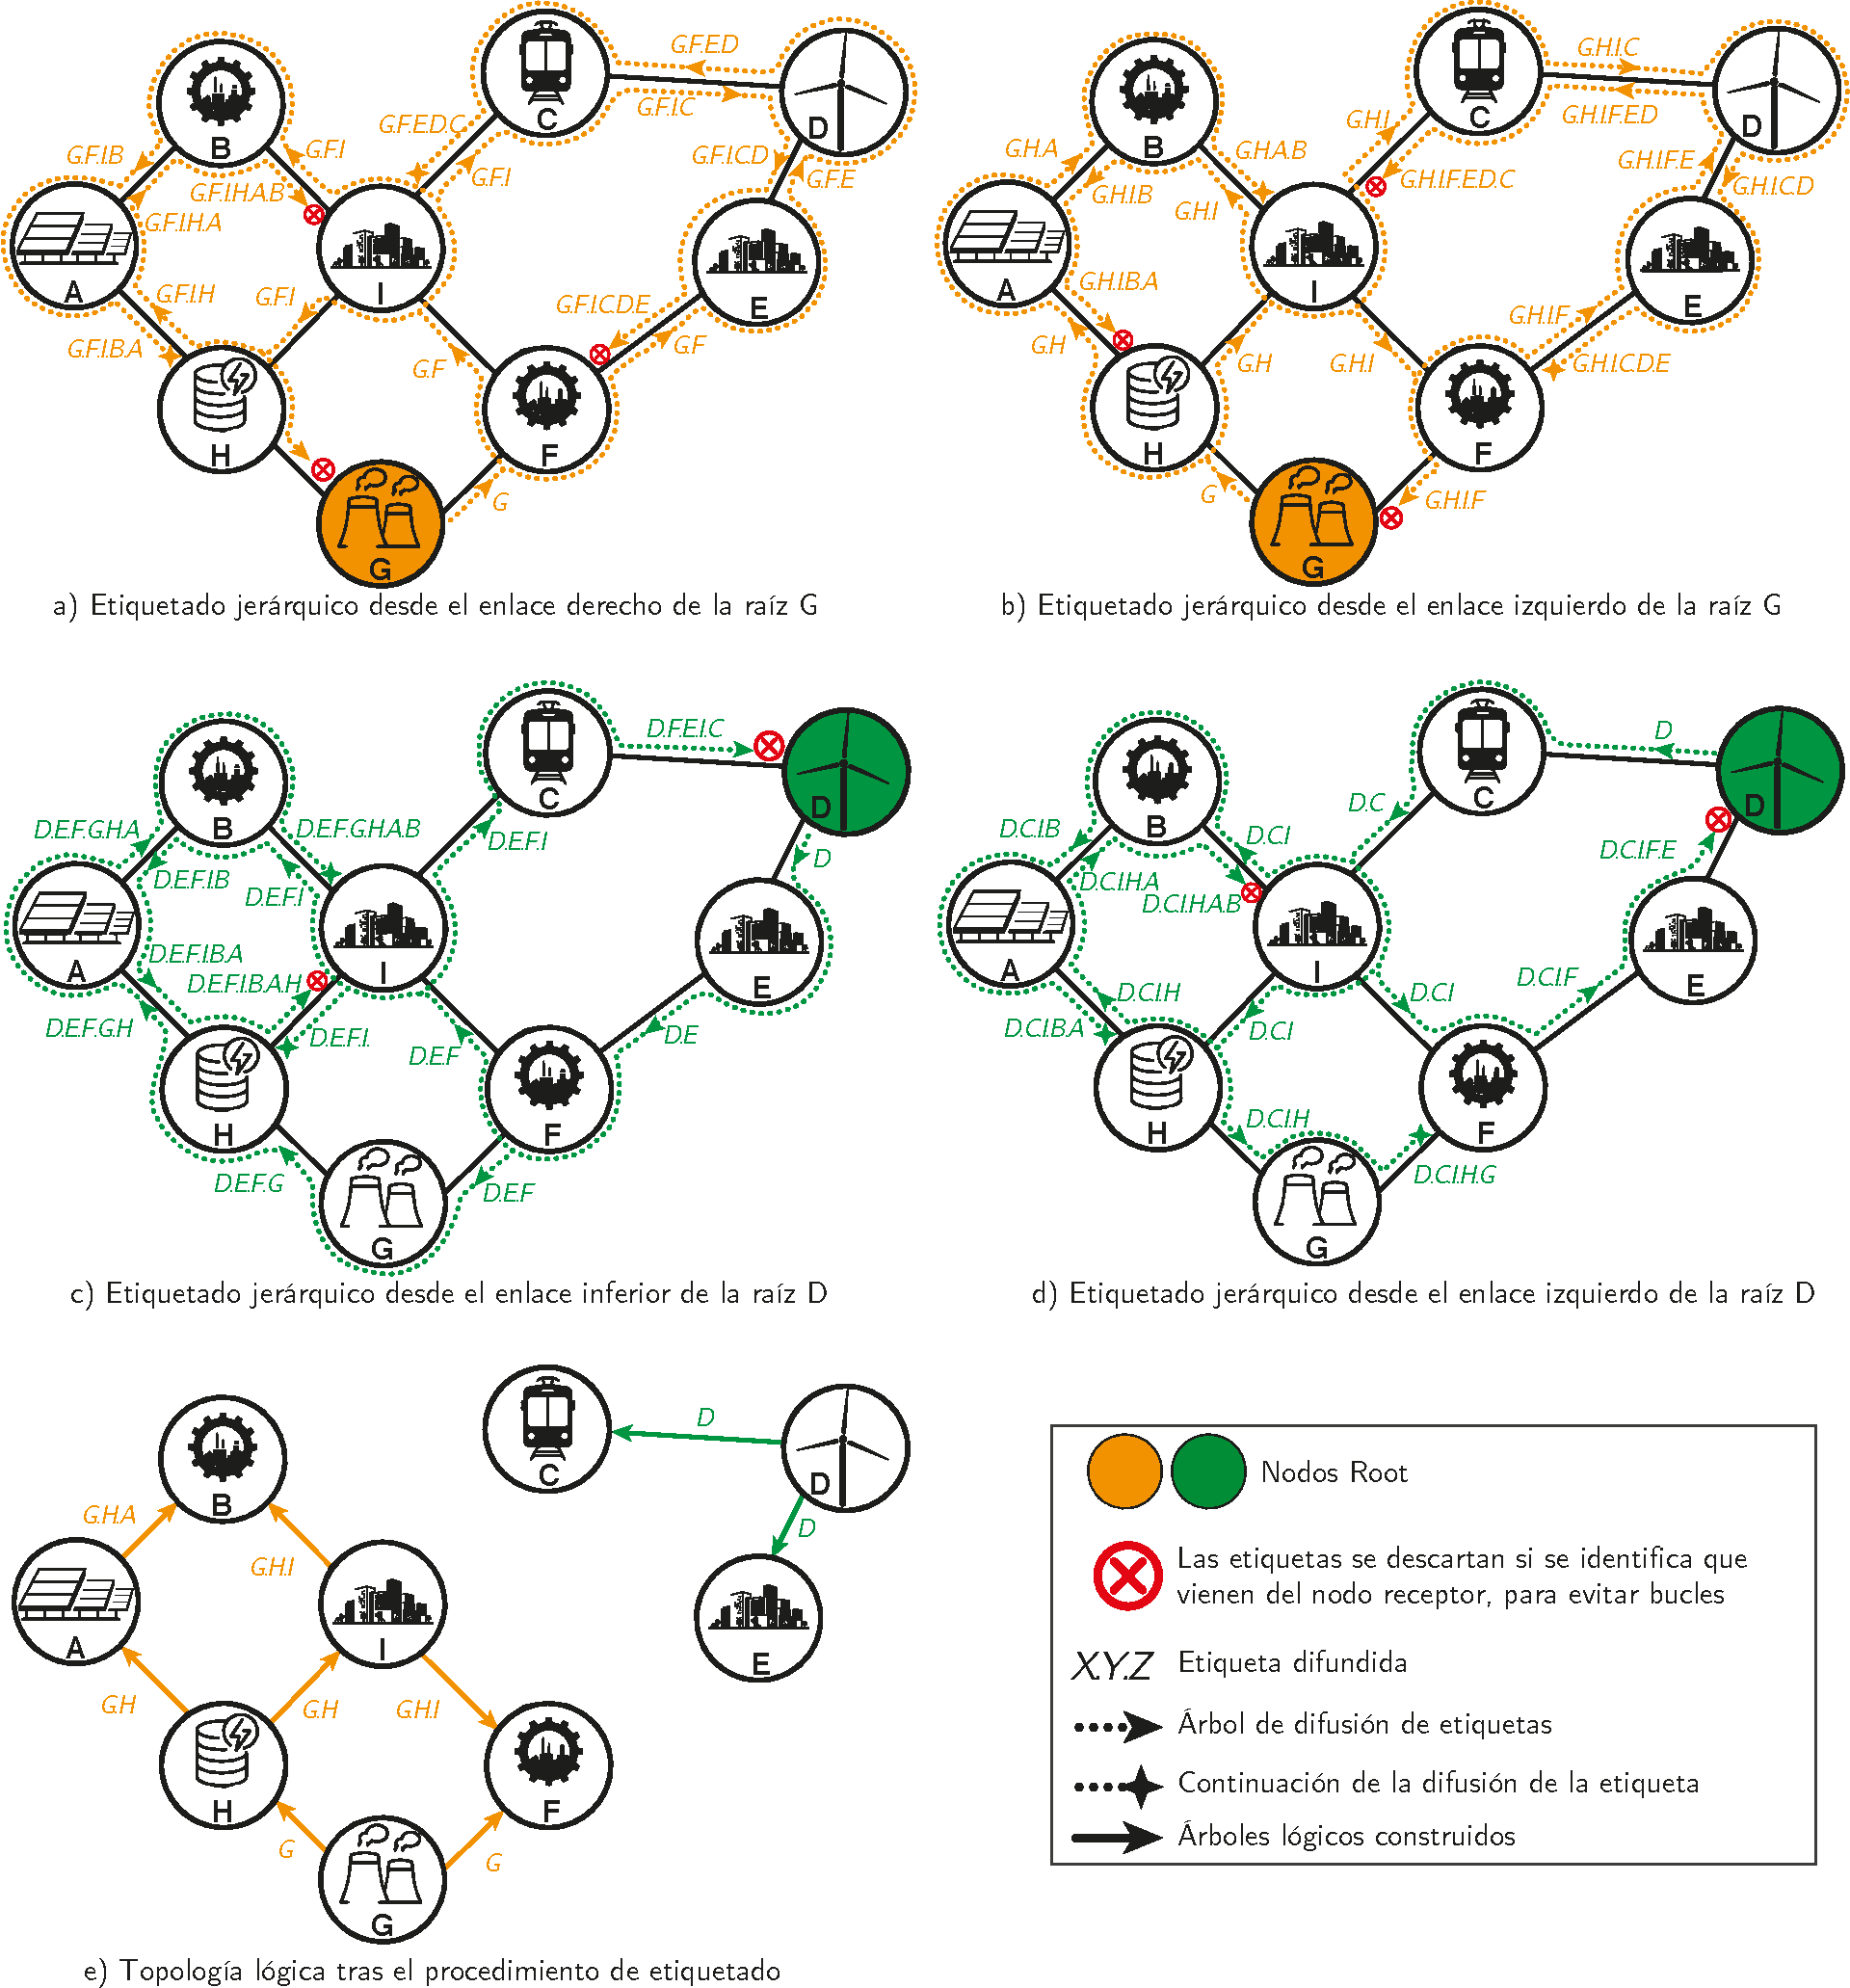
\includegraphics[width=\textwidth]{fig/07_bloste/bloste_03.pdf}
    \caption{Procedimiento de etiquetado jerárquico.}
    \label{fig:bloste_03}
\end{figure}

El proceso de difusión de etiquetas finaliza cuando toda la red ha sido explorada, asegurando que cada nodo recibe al menos una etiqueta jerárquica. En la práctica, cada etiqueta representa una ruta hacia el nodo raíz. Para evitar bucles durante la fase de etiquetado jerárquico, el algoritmo impide asignar etiquetas que contengan identificadores previamente recorridos. Esta precaución es sencilla de aplicar, ya que las etiquetas se generan concatenando los IDs de los nodos visitados, prohibiendo así la inclusión de IDs repetidos, lo cual indicaría un bucle. Por ejemplo, en la Figura~\ref{fig:bloste_03}a, el nodo \textit{I} descarta y finaliza el proceso de difusión de la etiqueta \textit{G.F.I.H.A.B}, dado que previamente había creado y difundido la etiqueta \textit{G.F.I}, que comparte el prefijo \textit{G.F.I}. Este mecanismo evita la formación de bucles y garantiza la construcción de un árbol jerárquico desde el nodo raíz. Para simplificar la representación de la figura, no se han incluido todos los procesos de difusión de etiquetas, los cuales se han señalado en el diagrama con una estrella de cuatro puntas.\\
\\
El proceso de difusión de etiquetas desde el enlace izquierdo del nodo raíz \textit{G}, mostrado en la Figura~\ref{fig:bloste_03}b, se desarrolla de manera similar. Este proceso genera otro subconjunto de rutas que forman un nuevo árbol complementario al anterior. El resultado final se resume en la Figura~\ref{fig:trees_from_root_node_G}, que muestra los dos árboles jerárquicos derivados del nodo raíz \textit{G}, seleccionando la ruta más rápida. En este sentido, cada nodo almacena dos etiquetas de diferentes árboles derivados del mismo nodo raíz. De este modo, cada nodo dispone de dos rutas alternativas para alcanzar el nodo raíz, que pueden seleccionarse en una fase posterior para construir la topología lógica de acuerdo con distintos criterios generales, como disyunción de rutas o número mínimo de saltos~\cite{Lopez-Pajares19,rojas2021outperforming}, o con criterios específicos de redes de distribución eléctrica, como el balance de potencia~\cite{Zishan2024} o las pérdidas energéticas~\cite{Zhang2024}.


\begin{figure*}[ht!]
\centering
\begin{minipage}{0.49\textwidth}
\centering
\begin{forest}
  for tree={grow=east, edge={-}, rounded corners}
  [G
    [F
        [I
            [H[A]]
            [C]
            [B]]
        [E[D]]]
  ]
\end{forest}
\\
\subcaption{Árbol jerárquico 1}
\end{minipage}
\hfill
\begin{minipage}{0.49\textwidth}
\centering
\begin{forest}
  for tree={grow=east, edge={-}, rounded corners}
  [G
    [H
        [I
            [F]
            [C[D[E]]]
            [A[B]]]]
  ]
\end{forest}
\subcaption{Árbol jerárquico 2}
\end{minipage}
\caption{Árboles jerárquicos tras el proceso de difusión del etiquetado desde el nodo raíz \textit{G}}
\label{fig:trees_from_root_node_G}
\end{figure*}



\subsubsection{Procedimiento de etiquetado jerárquico basado en múltiples árboles}

Las microrredes típicamente cuentan con múltiples puntos de acceso a la red de distribución eléctrica. Estos puntos de acceso permiten la reconfiguración de la red mediante el control de interruptores para optimizar métricas de operación, manteniendo al mismo tiempo una operación segura y estable~\cite{wang2020research,zhaoyu2012multi}. Es por ello, que en este escenario puede ser visto como un grafo con varios nodos que conectan la microrred a la red de distribución eléctrica, designados como raíces. Cada raíz debería tener uno o más árboles jerárquicos para distribuir la energía a los nodos según la oferta o demanda de la microrred. Por lo tanto, es posible construir múltiples árboles jerárquicos a partir de varios nodos raíz.\\
\\
El mecanismo presentado en este trabajo permite ejecutar múltiples procedimientos de difusión de etiquetas desde varios nodos raíz simultáneamente, proporcionando múltiples caracterizaciones de la topología de la red desde diferentes nodos raíz al mismo tiempo. Las Figuras~\ref{fig:bloste_03}c y ~\ref{fig:bloste_03}d muestran el procedimiento de difusión de etiquetas desde un nuevo nodo raíz \textit{D}. Este proceso podría ejecutarse al mismo tiempo que el procedimiento de difusión de etiquetas desde el nodo \textit{G} descrito anteriormente. Ambos procesos son independientes y no interfieren entre sí. Dado que la etiqueta raíz difundida desde cada nodo raíz es diferente, los procedimientos derivados de cada uno son independientes y pueden coexistir en el tiempo. A partir de este nuevo nodo raíz, se obtienen dos árboles jerárquicos adicionales, seleccionando la ruta más rápida, como se muestra en la Figura~\ref{fig:trees_from_root_node_D}.

\begin{figure*}[ht!]
\centering
\begin{minipage}{0.49\textwidth}
\centering
\begin{forest}
  for tree={grow=east, edge={-}, rounded corners}
  [D
    [E
        [F
            [I
            [C]]
            [G[H[A]]]]
  ]]
\end{forest}
\\
\subcaption{Árbol jerárquico 1}
\end{minipage}
\hfill
\begin{minipage}{0.49\textwidth}
\centering
\begin{forest}
  for tree={grow=east, edge={-}, rounded corners}
  [D
    [C
        [I
            [H[G]]
            [F[E]]
            [B[A]]]]
  ]
\end{forest}
\subcaption{Árbol jerárquico 2}
\end{minipage}
\caption{Árboles jerárquicos tras el proceso de difusión del etiquetado desde el nodo raíz \textit{D}}
\label{fig:trees_from_root_node_D}
\end{figure*}

Una vez que todas las etiquetas de ambos nodos raíz han sido difundidas, se dispone de varias caracterizaciones de la topología física. La topología lógica puede construirse entonces utilizando uno o más de los criterios definidos en la Sección~\ref{subsec:criteria}. En el ejemplo ilustrado en la Figura~\ref{fig:bloste_03}e, se crean dos ``islas'' de energía, una que involucra los nodos \textit{D,C,E} y otra que involucra al resto de los nodos. Sin embargo, dependiendo de los criterios de optimización seleccionados, la topología resultante podría ser diferente.


\subsection{Criterios para construir la topología lógica}
\label{subsec:criteria}
% Meter los criterior a fuegoooooo :) 

Como se introdujo anteriormente, una vez concluido el procedimiento de etiquetado, todos los nodos pueden utilizar cualquiera de las etiquetas asignadas para alcanzar el nodo raíz, ya que las etiquetas delinean implícitamente la secuencia de nodos que deben recorrerse para llegar hasta la raíz. Cuando un nodo está asociado únicamente a una etiqueta, existe un único camino hacia la raíz. Sin embargo, si existen múltiples etiquetas, se deben emplear criterios específicos para seleccionar la ruta más óptima hacia la raíz. En consecuencia, la segunda fase del algoritmo determina la distribución de potencia aplicando criterios predefinidos de acuerdo con el orden establecido por las etiquetas o los identificadores jerárquicos\footnote{Nótese que, a partir de este punto, ID representa identificadores jerárquicos o etiquetas, es decir, aquellos derivados del proceso de etiquetado previo (no los IDs únicos de los nodos).} configurados durante la primera fase.\\
\\
Cada etiqueta \( ID \) se define formalmente como una secuencia ordenada de \( k + 1 \) nodos que representan un camino válido desde un nodo dado \( n_k \in \mathcal{N}' \) hasta el nodo raíz \( n_0 \in \mathcal{N}' \), atravesando la topología lógica \( G' = (\mathcal{N}', \mathcal{L}') \). Es decir,

\begin{equation}
\begin{aligned}
    ID &= \{n_0, n_{1}, \dots, n_{k-1}, n_k\}, \\
    &\quad \text{con} \quad (n_{l-1},n_{l}) \in \mathcal{L}', \: \forall l \in \{1, \dots, k\}.
\end{aligned}
\end{equation}
\vspace{0.2cm}

En esta definición, el índice 0 siempre corresponde al nodo raíz, y el índice \( k \) al nodo de origen (es decir, el nodo desde el cual se evalúa el ID). Esta notación facilita la evaluación consistente de cada ruta y la aplicación de criterios que dependen del número de saltos o de las características de los enlaces recorridos.\\
\\
Como referencia, nuestro algoritmo ofrece cuatro criterios distintos para seleccionar la ruta óptima para la distribución de energía hacia la raíz. Cada criterio considera diversos aspectos topológicos y características de despliegue para calcular un coste para cada ruta disponible, denotado como el coste asociado a cada identificador jerárquico ($Cost\_{ID}$).\\
\\
Posteriormente, el algoritmo identifica la ruta óptima, la etiqueta activa o el identificador jerárquico activo ($ID\_{activa}$) en función del coste mínimo, tal como se especifica en la Ecuación~\ref{eq:IDactiveCost}. Los cuatro criterios se describen en las secciones siguientes; no obstante, es posible definir criterios adicionales e incorporarlos al algoritmo, dado que esta segunda fase únicamente requiere la definición de una función de coste para cada criterio, sin estar limitada a una implementación específica. Por lo tanto, el criterio para la selección de $ID_{active}$ se mantiene constante para todos los criterios presentados; lo que varía es el método utilizado para calcular el coste asociado a cada ruta según el criterio aplicado.

\subsubsection{Número de saltos}
\label{subsec:criteria_01}

En este primer criterio (\textit{Hops}) se considera el número de saltos necesarios para alcanzar el nodo raíz. Este criterio coincide con el descrito en \gls{d2e} (ver Sección~\ref{subsec:fase2}), por lo que aquí se presenta de manera resumida utilizando la notación adoptada en esta propuesta. Cada identificador jerárquico se define como una secuencia \( ID = \{n_0, n_{1}, \dots, n_{k-1}, n_k\} \), donde \( n_0 \) corresponde al nodo raíz y \( n_k \) al nodo de origen. El número de saltos se determina por la cantidad de enlaces recorridos a lo largo del camino desde el nodo de origen hasta la raíz, lo que equivale al número de nodos en la secuencia menos uno. Por lo tanto, se selecciona la etiqueta que minimice el número de saltos hacia el nodo raíz. El coste asociado a este criterio puede expresarse de la siguiente manera:

\begin{equation}
     Cost_{ID}  \: = \: \text{length}(ID) - 1 \: = \: k
\end{equation}

donde \( \text{length}(ID) \) indica el número de nodos en la secuencia (es decir, \( k+1 \)), y el coste resultante \( k \) representa el número total de saltos desde el nodo de origen \( n_k \) hasta el nodo raíz \( n_0 \).

\subsubsection{Bajas pérdidas de enlace}
\label{subsec:criteria_02}

Este segundo criterio (\textit{Low-Link Losses}) establece una relación entre las características físicas de las líneas de transmisión y la distancia lógica al nodo raíz. Su objetivo es minimizar las pérdidas totales de propagación que afectan a la potencia incidente en cada línea, considerando también el número de saltos a lo largo del camino. La lógica detrás de este enfoque consiste en optimizar la distribución de energía favoreciendo tanto rutas físicamente eficientes como aquellas que, desde un punto de vista lógico, acercan la carga al nodo raíz, promoviendo así la agregación hacia el sumidero central. En las redes inteligentes, las pérdidas ($L_{n_{l-1},n_l}$) se calculan utilizando modelos de pérdida de líneas de transmisión que incorporan parámetros intrínsecos como el voltaje de operación ($V_{d}$), la distancia física del enlace ($d_{n_{l-1}, n_l}$), el coeficiente de reflexión ($\alpha_{R_{n_{l-1},n_l}}$) y la potencia incidente en la línea ($P_{in}$), tal como se expresa en la Ecuación~\ref{eq:criterionCost04_b_bloste}. Es evidente que la distancia física constituye un factor clave que influye en el coste total; no obstante, otros parámetros intrínsecos de la línea de transmisión, como los coeficientes de reflexión y el voltaje de operación, también desempeñan un papel relevante.

\begin{equation}\label{eq:criterionCost04_b_bloste}
     L_{n_{l-1},n_l} \: = \: \frac{\alpha_{R_{n_{l-1},n_l}} \: \times \: d_{n_{l-1},n_l}}{V_{d}^{2}}\: \times \: P_{in}^{2}
\end{equation}
\vspace{0.2cm}

Adicionalmente, se considera la distancia lógica al nodo raíz, incentivando, en cierta medida, que la inercia de la carga se dirija hacia el sumidero principal de la topología, es decir, el nodo raíz. Al analizar la Ecuación~\ref{eq:criterionCost02_bloste}, se observa que se introducen dos parámetros de configuración, $\alpha$ y $\beta$, para regular la importancia relativa de las pérdidas de propagación dentro de la función de coste, así como de la distancia lógica al nodo raíz. Por defecto, ambos parámetros se establecen en $0.5$, garantizando un equilibrio igualitario entre estos dos factores. No obstante, es posible explorar una optimización adicional de estos valores dependiendo del tipo específico y los requisitos de las redes en las que se implemente este criterio. El número de saltos a lo largo del camino es \( k \), y las pérdidas de propagación se calculan para cada enlace \( (n_{l-1}, n_l) \in \mathcal{L}' \) utilizando la expresión~\ref{eq:criterionCost04_b_bloste}.

\begin{equation}\label{eq:criterionCost02_bloste}
     Cost_{ID}  \: = \: \alpha \cdot k \: + \: \beta \cdot \sum_{l=k}^{1} \left( \frac{\alpha_{R_{n_{l-1},n_l}} \cdot d_{n_{l-1},n_l}}{V_{d}^{2}} \cdot P_{in}^{2} \right)
\end{equation}

\subsubsection{Balance de potencia local a cero}
\label{subsec:criteria_03}

Este tercer criterio (\textit{Power2Zero}) se centra en optimizar el equilibrio de potencia local entre nodos vecinos, con el objetivo de minimizar o incluso eliminar el intercambio neto de potencia entre ellos. Este concepto resulta fundamental en el contexto de las \gls{der}, ya que fomenta la autosuficiencia local: los nodos vecinos procuran cubrir colectivamente su demanda sin depender del nodo raíz ni de la red principal. Al lograr esta compensación local, el sistema reduce significativamente la necesidad de transportar energía a través de la red primaria, lo que a su vez disminuye las pérdidas de transmisión y alivia la presión sobre la infraestructura en su conjunto. Este enfoque no solo mejora la eficiencia energética, sino que también se alinea con el objetivo estratégico de la generación distribuida: satisfacer la demanda local mediante recursos locales. En consecuencia, contribuye a diferir o incluso evitar costosas expansiones de la red y fortalece la sostenibilidad y escalabilidad del sistema eléctrico.\\
\\
Para abordar este criterio, tal como se ilustra en la Ecuación~\ref{eq:criterionCost03_bloste}, cada nodo evalúa los estados de potencia actuales de sus vecinos y determina qué configuración aproxima más el balance a cero. De manera análoga al criterio anterior, se introducen los parámetros $\alpha$ y $\beta$ (ambos fijados inicialmente en $0.5$), junto con el componente de distancia lógica al nodo raíz de la topología. Este planteamiento permite ponderar de manera configurable cada componente de la función de coste, posibilitando tanto la optimización del equilibrio de potencia en mínimos locales como la priorización de la distancia lógica hacia el nodo de acceso a la red. De este modo, se fomenta un flujo de potencia inherente hacia el punto de conexión de la red de distribución.  

\begin{equation}\label{eq:criterionCost03_bloste}
       Cost_{ID}  \: = \: \alpha \cdot k + \: \beta (|P_{k-1} + P_{k}|) 
\end{equation}


Al igual que en los criterios anteriores, esta función de coste se aplica a todas las secuencias $ID$ disponibles asociadas al nodo de origen ($n_{k}$). Ello permite identificar al vecino inmediato ($n_{k-1}$) cuyo equilibrio de potencia se vea más favorecido, es decir, más próximo a cero, incorporando al mismo tiempo un componente de ponderación configurable que orienta gradualmente las cargas hacia el nodo raíz de la topología.

\subsubsection{Balance de potencia local a cero con pérdidas}
\label{subsec:criteria_04}


El cuarto criterio (\textit{Power2Zero + Losses}) busca integrar los parámetros evaluados previamente, a saber: el balance de potencia local y las pérdidas derivadas del proceso de compensación. Tal como se ilustra en la Ecuación~\ref{eq:criterionCost04_bloste}, este criterio evalúa cada secuencia jerárquica \( ID = \{n_0, n_1, \dots, n_k\} \), considerando los estados de potencia de los dos últimos nodos de la secuencia, \( n_{k} \) (nodo de origen) y \( n_{k-1} \) (vecino a un salto), e incorporando además la pérdida de transmisión \( L_{n_{k-1}n_k} \) asociada al último enlace. El coste resultante se define como:

\begin{equation}\label{eq:criterionCost04_bloste}
      Cost_{ID} \: = \: |P_{n_k} + P_{n_{k-1}} - L_{n_{k-1}n_k}|
\end{equation}
\vspace{0.05cm}

Esta formulación combina de manera efectiva los componentes clave de los criterios presentados en las Secciones~\ref{subsec:criteria_03} y~\ref{subsec:criteria_02}, al evaluar conjuntamente la compensación local y la eficiencia en la transmisión sobre el tramo final de la ruta. De este modo, se fomenta un intercambio de potencia local que no solo favorece la autosuficiencia, sino que también incorpora la conciencia de pérdidas, mejorando la robustez y la eficiencia global del sistema.

\subsection{Balanceo utilizando la topología lógica}
\label{subsec:iterativeBalance}

Una vez que las etiquetas han sido propagadas a lo largo de la topología y se ha aplicado el criterio de selección, cada nodo obtiene un $ID_{activa}$, lo que permite establecer la topología lógica y dar inicio al procedimiento de balanceo global de potencia. Este proceso posibilita la redistribución de las cargas, comenzando en los nodos más periféricos de la red y avanzando progresivamente hacia el nodo raíz, mientras se favorece de manera simultánea el balanceo localizado entre nodos adyacentes.


\begin{figure}[ht!]
    \centering
    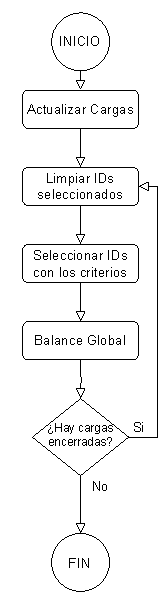
\includegraphics[width=0.28\textwidth]{fig/07_bloste/bloste_04.pdf}
    \caption{Balanceo de potencia mediante topología lógica: un enfoque iterativo}
    \label{fig:iterativeBalance}
\end{figure}

Se ha concebido un enfoque iterativo para llevar a cabo un balanceo sistemático de las cargas de potencia a lo largo de la topología, tal como se ilustra en la Figura~\ref{fig:iterativeBalance}. En cada iteración, tras la actualización de la configuración de cargas, cada nodo debe determinar una nueva $ID_{activa}$, desactivando el identificador previamente asignado. Esta reevaluación resulta fundamental para identificar dinámicamente la ruta óptima en función de la distribución de carga vigente. Sin embargo, dado el carácter estático de la topología física, no es necesario realizar una reexploración de las rutas. \\
\\
Una vez que las $ID_{activa}$ han sido reasignadas a nivel de nodo y se ha activado el identificador óptimo, el proceso de balanceo de potencia prosigue conforme a la topología lógica. De esta manera, se garantiza un equilibrio local de potencia, canalizando cualquier demanda o excedente residual hacia el nodo raíz. El proceso iterativo continúa hasta que no exista demanda ni excedente dentro de la topología (es decir, hasta que no queden cargas internas por compensar), lo que señala la resolución completa de los desbalances, con la excepción del nodo raíz, que refleja el balance global correspondiente a cada iteración.\\
\\
En cada iteración del proceso de balanceo global se registran dos métricas fundamentales: el balance total de potencia de la topología ($total\_balance$) y la magnitud absoluta del flujo de potencia en el sistema ($abs\_flux$). La suma acumulada de estas métricas a lo largo de todas las iteraciones ofrece una medida integral tanto del flujo absoluto de potencia como del balance total alcanzado en la topología. El procedimiento de balanceo global de potencia se repite cada vez que se detecta una nueva configuración de cargas, es decir, en cada intervalo de actualización (\emph{delta time}) de las cargas. Los resultados obtenidos y sus implicaciones se presentan en la Sección~\ref{sec:evaluation_bloste}. Conviene destacar que este enfoque iterativo se ha empleado únicamente con fines de validación conceptual de la propuesta. No obstante, es previsible que en implementaciones prácticas pueda adoptar variantes, en función del contexto específico de despliegue, como se analizará en la Sección~\ref{susec:pracImpl}, dedicada a las implicaciones prácticas.


\subsection{Resiliencia y tasa de refresco}

La construcción de la topología lógica basada en etiquetas proporciona de manera inherente resiliencia frente a eventos disruptivos o fallos en la red. Esta resiliencia surge de la disponibilidad de múltiples etiquetas por nodo, siempre que exista más de un camino hacia el nodo raíz, lo que permite la reconfiguración dinámica de las rutas activas en respuesta a degradaciones de enlace, pérdidas de conectividad o fallos parciales del sistema. En este contexto, cuando un nodo detecta la pérdida de un enlace con su nodo ascendente en la topología lógica, o cuando los parámetros de calidad del enlace (como las pérdidas de propagación o el balance de potencia) se degradan por debajo de umbrales predefinidos, puede activar una reevaluación de sus etiquetas alternativas. Al reaplicar los criterios de selección detallados en la Sección~\ref{subsec:criteria}, el nodo puede escoger una nueva $ID_{activa}$ que represente un camino más adecuado hacia el nodo raíz bajo las condiciones actuales de la red. Este mecanismo automático de conmutación de rutas permite una adaptabilidad continua sin necesidad de rediseñar o redistribuir completamente la topología lógica, preservando así la continuidad del servicio y la estabilidad de la red.\\
\\
Adicionalmente, con el fin de garantizar un comportamiento de red óptimo y actualizado, se ha definido una tasa de refresco periódica para evaluar, a intervalos regulares, la validez de la ruta activa seleccionada ($ID_{activa}$). Esta tasa de refresco está parametrizada mediante un temporizador $T_{refresh}$, que desencadena la reevaluación de los costes asociados a todas las etiquetas disponibles. En función de la dinámica del sistema (por ejemplo, variaciones en la demanda de potencia o la aparición de nuevas fuentes), este temporizador puede configurarse con valores más agresivos (para entornos altamente dinámicos) o más conservadores (para escenarios estables), equilibrando de este modo la capacidad de respuesta del sistema con el coste computacional del recálculo de rutas. \\
\\
Cabe señalar que este mecanismo de refresco puede coexistir con un esquema reactivo, en el cual eventos externos, como la desconexión de nodos o la aparición de sobrecargas, también pueden activar una reevaluación inmediata de rutas sin esperar a la expiración del temporizador $T_{refresh}$. En conjunto, estos dos mecanismos, tanto proactivo como reactivo, garantizan una operación robusta, eficiente y adaptable del sistema tanto ante condiciones previstas como imprevistas.

\subsection{Implicaciones prácticas}
\label{susec:pracImpl}

La implementación de la arquitectura propuesta, basada en el etiquetado jerárquico y en topologías lógicas multi-raíz, presenta implicaciones directas y significativas para su despliegue en sistemas eléctricos reales. Para materializar estas técnicas en entornos físicos, resulta esencial la integración de \glspl{er}. Estos dispositivos constituyen un pilar fundamental dentro del paradigma de la \gls{ei}, al permitir no solo la conversión y el intercambio de energía, sino también el encaminamiento inteligente y la toma de decisiones autónoma en cada nodo de la red~\cite{benchikh2024survey}. Los \glspl{er} deben ser capaces de ejecutar algoritmos distribuidos de encaminamiento energético, interpretar etiquetas jerárquicas y evaluar múltiples trayectorias en función de criterios dinámicos como las pérdidas de transmisión, el balance de potencia local o la distancia topológica.\\
\\
En un sistema real, la presencia de múltiples nodos raíz, tales como puntos de interconexión con la red principal o centros de generación renovable, exigiría la construcción simultánea de diversas superposiciones lógicas. Esta capacidad permitiría a los servicios de operación seleccionar en tiempo real la ruta más adecuada para satisfacer la demanda o evacuar la generación, teniendo en cuenta el estado actual y las condiciones previstas de la red. De este modo, se logra una mayor flexibilidad operativa, ya que el sistema puede adaptarse dinámicamente a cambios en la carga, la generación, la topología o la aparición de fallos sin requerir un control centralizado.\\
\\
Asimismo, la posibilidad de operar sobre múltiples árboles mediante criterios configurables ofrece una ventaja decisiva en términos de eficiencia energética y resiliencia. Permite al sistema minimizar las pérdidas, aliviar la congestión de los enlaces y mejorar la utilización de los recursos energéticos locales. La lógica de decisión distribuida propuesta en este trabajo es coherente con las tendencias actuales en eficiencia energética, que buscan maximizar el uso de la energía local, reducir los intercambios con la red principal y fomentar la autosuficiencia energética entre nodos vecinos.\\
\\
En última instancia, el despliegue práctico de esta arquitectura requiere un ecosistema tecnológico alineado con los principios de la \gls{ei}, en el cual los \glspl{er} funcionen no solo como interfaces físicas de los componentes de generación, almacenamiento y consumo, sino también como agentes inteligentes capaces de gestionar de manera autónoma los flujos energéticos. Tal como se enfatiza en~\cite{Fawaz2025}, este enfoque representa un paso fundamental hacia la transición desde redes eléctricas tradicionales hacia infraestructuras energéticas distribuidas, adaptativas y sostenibles, en consonancia con los objetivos de largo plazo del paradigma de la \gls{ei}. En última instancia, será responsabilidad del operador de red que implemente dicho paradigma determinar cómo configurar los criterios de selección, cuáles aplicar en cada nodo y cuáles priorizar en distintos momentos del día, de acuerdo con las necesidades específicas de la red. Además, el operador deberá garantizar la coherencia entre los criterios aplicados en todo el sistema para evitar conflictos y asegurar una toma de decisiones consistente.


\section{Evaluación}
\label{sec:evaluation_bloste}

Para evaluar nuestro algoritmo, en una primera instancia se empleó la topología de referencia \gls{ieee} 123-Node Test Feeder. No obstante, tras el proceso de revisión por pares, se consideró necesario ampliar el alcance de la evaluación incorporando la topología \gls{ieee} 34-bus, así como realizar un análisis de la complejidad computacional asociado a las fases de etiquetado jerárquico y balanceo iterativo. Este último análisis resulta fundamental para comprender cómo escalan los bloques principales del algoritmo bajo diferentes tamaños de topologías. Por tanto, las evaluaciones desarrolladas en este trabajo se estructuran de la siguiente manera:

\begin{itemize}
    \item \textbf{Evaluación sobre la topología \gls{ieee} 123-Node Test Feeder.} Se analiza el comportamiento del algoritmo fijando un nodo específico como raíz, así como aplicando el procedimiento de manera sucesiva considerando a cada nodo de la topología como nodo raíz. Esta aproximación permite obtener una visión promediada del comportamiento del algoritmo.

    \item \textbf{Evaluación sobre la topología \gls{ieee} 34-bus.} Se examina la capacidad del algoritmo para operar en una red de distribución con características distintas, ampliando así la validación de su aplicabilidad.

    \item \textbf{Estudio de la complejidad computacional.} Se realiza un análisis detallado de los dos bloques principales del algoritmo: etiquetado jerárquico; y balanceo iterativo, con el fin de caracterizar su escalabilidad y coste computacional.
\end{itemize}



\subsection{Evaluación sobre la topología IEEE 123-Node Test Feeder}

El \gls{ieee} 123-Node Test Feeder es un sistema teórico de distribución eléctrica ampliamente utilizado para evaluar el desarrollo de estrategias, tecnologías o algoritmos de gestión en redes de potencia~\cite{Schneider17}.\\
\\
Este sistema, desarrollado por el \gls{ieee}, está compuesto por un conjunto de nodos, o puntos de conexión, interconectados dentro de una red típica de distribución en baja tensión. Tal como se ilustra en la Figura~\ref{fig:ieeeNodeTestFeeder}, la red de prueba incorpora un total de 11 interruptores, lo que permite la reconfiguración de la red en función de las necesidades operativas. Detalles adicionales sobre las características de las líneas y de las cargas pueden encontrarse en \cite{Schneider17}. Considerando que los interruptores pueden encontrarse en estado abierto o cerrado, existen 2048 ($2^{11}$) posibles configuraciones de conmutación, excluyendo la direccionalidad de cada enlace. \\
\\
Para modelar los enlaces de la red, se han adoptado las configuraciones descritas en \cite{Schneider17}. Estas configuraciones pueden clasificarse en tres tipos de enlace distintos (véase la Tabla~\ref{tab:links}), en función de la resistencia ($\frac{ohm}{km}$), la sección transversal ($mm^{2}$) y la capacidad máxima de corriente ($A$). Las configuraciones recogidas en la Tabla~\ref{tab:links} se aplican a cada enlace de la topología IEEE 123-Node Test Feeder, escalando las pérdidas a un 8\% y triplicando la capacidad cuando se manejan valores de carga trifásicos. Este ajuste sigue las especificaciones de \cite{Schneider17}, donde a cada enlace se le asigna una configuración predefinida.\\


\begin{figure}[ht!]
    \centering
    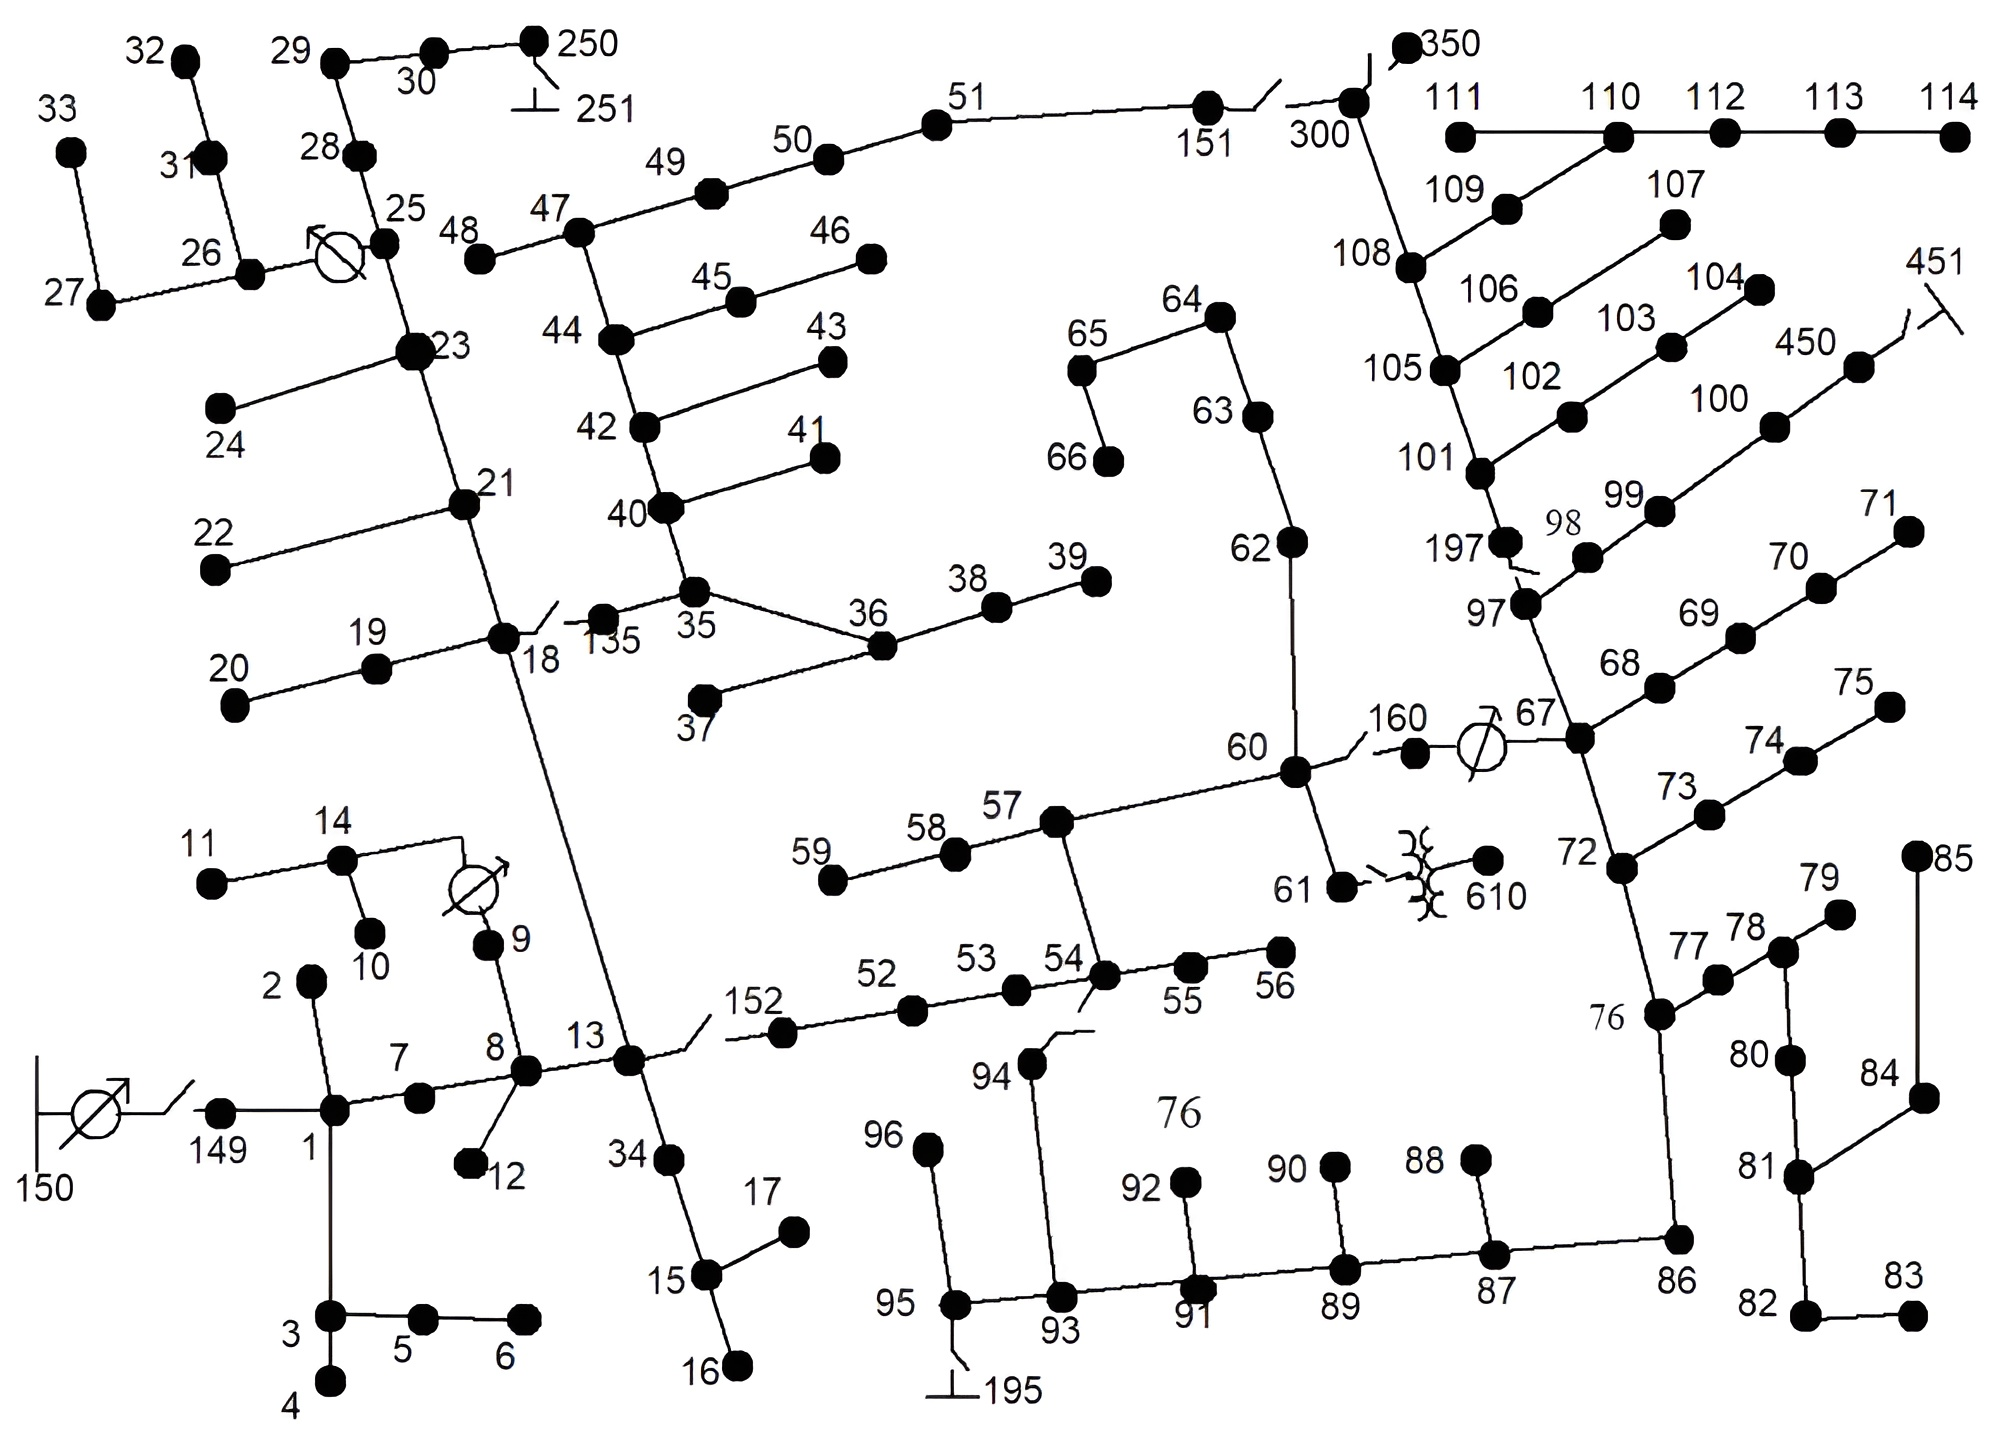
\includegraphics[width=0.7\textwidth]{fig/07_bloste/bloste_05.png}
    \caption{Topología IEEE 123-Node Test Feeder~\cite{Schneider17}.}
    \label{fig:ieeeNodeTestFeeder}
\end{figure}


Con respecto a la configuración de cargas de la topología, se emplearon las cargas especificadas en los perfiles de nodo detallados en \cite{Schneider17}. De acuerdo con la definición de la topología, existen dos tipos de nodos: nodos finales, que en cada instante pueden generar o demandar potencia, y nodos virtuales, que actúan como puntos de interconexión dentro de la topología pero que no generan ni demandan potencia en el estado inicial. Para evaluar el rendimiento de nuestro algoritmo, se han considerado 95 instantes de tiempo distintos, en los cuales cada nodo final presenta una potencia instantánea diferente, siempre coherente con el perfil definido en la descripción de la topología. Con el fin de ofrecer una representación más clara de los distintos perfiles de carga, la Figura~\ref{fig:loadsHist} muestra el histograma global de los perfiles de carga de todos los nodos de la topología. Asimismo, la Figura~\ref{fig:loads_global_view} ilustra la generación, el consumo y el balance de potencia a lo largo del conjunto completo de nodos de la topología.\\
\\
Como puede observarse en la Figura~\ref{fig:loadsHist}, el perfil medio de potencia de los nodos finales tiende a concentrarse en valores negativos, lo cual implica que los resultados de los cálculos de balance de potencia realizados dentro de la topología serán, con alta probabilidad, negativos. En otras palabras, la red tenderá, en promedio, a demandar potencia de la red de distribución. Tal como se ilustra en la Figura~\ref{fig:loads_global_view}, la topología presenta predominantemente una configuración de cargas globales negativas a lo largo del día. Por tanto, será de importancia crítica evaluar el desempeño de los criterios con respecto a la variación neta en los balances de potencia durante los momentos del día en los que se produzcan picos de generación.

\begin{figure}[ht!]
    \centering
    \begin{subfigure}{0.45\textwidth}
        \centering
        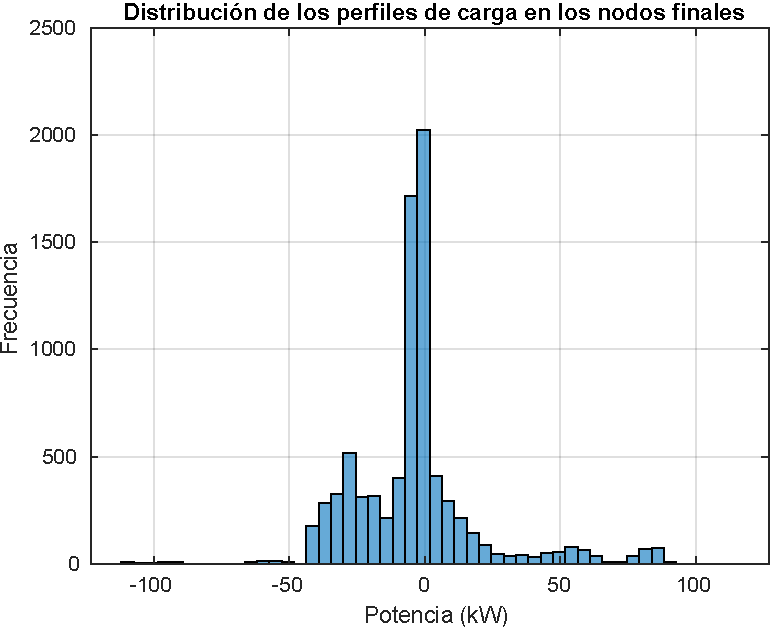
\includegraphics[width=\textwidth]{fig/07_bloste/bloste_06a.pdf}
        \caption{Histograma de la distribución de los perfiles de carga de los nodos finales.}
        \label{fig:loadsHist}
    \end{subfigure} \hspace{0.05\textwidth}
    \begin{subfigure}{0.45\textwidth}
        \centering
        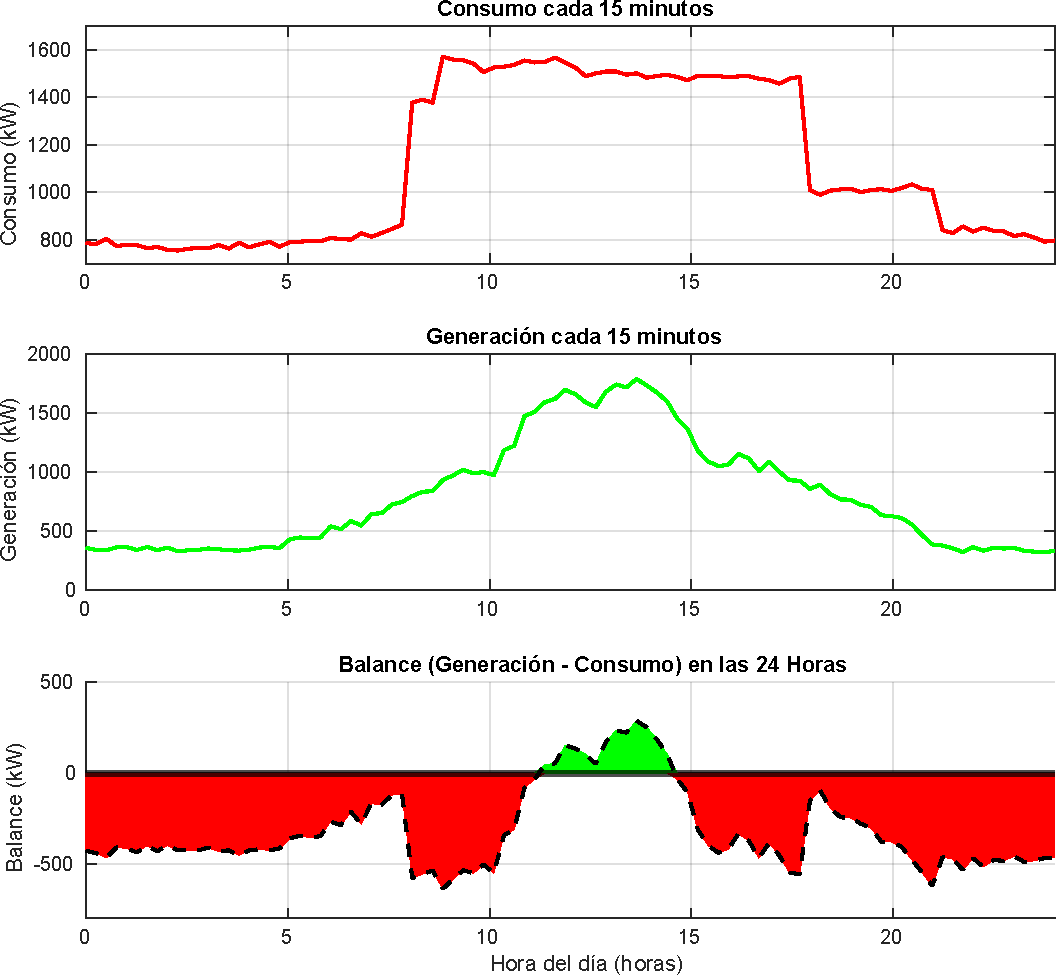
\includegraphics[width=\textwidth]{fig/07_bloste/bloste_06b.pdf}
        \caption{Perfiles generales de consumo, generación y balance durante el día.}
        \label{fig:loads_global_view}
    \end{subfigure}
    \caption{Caracterización de la configuración de carga utilizada en la Topología IEEE 123-Node Test Feeder.}
\end{figure}

Para la evaluación de nuestro algoritmo, la red \gls{ieee} 123-Node Test Feeder ha sido simulada en Python. Se seleccionó Python por su versatilidad, flexibilidad y su amplia adopción en la comunidad científica. Se evitó deliberadamente el uso de librerías externas, basando toda la implementación únicamente en las librerías estándar de Python, con el fin de minimizar la complejidad y reducir posibles errores derivados de dependencias entre paquetes externos. La simulación de la topología se implementó empleando \gls{oop}, estableciendo una jerarquía de clases (véase la Figura~\ref{fig:uml}). 

\begin{figure}[ht!]
    \centering
    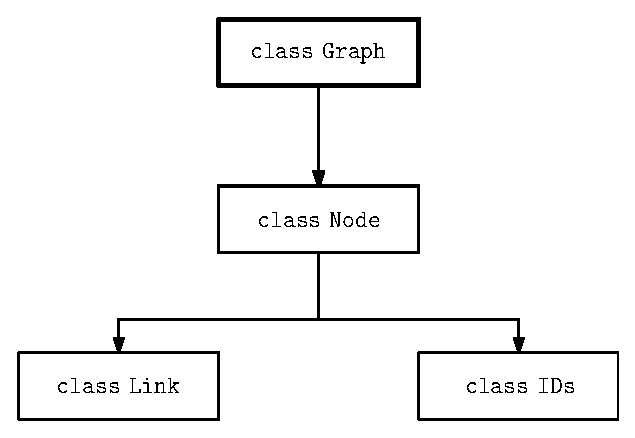
\includegraphics[width=0.45\textwidth]{fig/07_bloste/bloste_07.eps}
    \caption{Jerarquía de clases para simular la Topología IEEE 123-Node Test Feeder.}
    \label{fig:uml}
\end{figure}

Dicha jerarquía incluye una clase de grafo, que contiene una lista de objetos nodo. Cada objeto nodo, a su vez, incorpora objetos enlace para representar sus relaciones con los nodos vecinos. Adicionalmente, los objetos nodo contienen objetos ID destinados a almacenar las etiquetas del algoritmo, permitiendo así identificar la posición de cada nodo dentro del o de los árboles.\\
\\
La evaluación del algoritmo se ejecutó en 96 instantes temporales distintos, en los cuales los nodos finales de la topología partieron de diferentes condiciones de carga, ya fuera en régimen de consumo o de generación, siguiendo el perfil medio de potencia representado en la Figura~\ref{fig:loads_global_view}. Las simulaciones se realizaron en un servidor de alto rendimiento con un Ubuntu 22.04, equipado con un procesador Intel(R) Core(TM) i9 y 32 GB de memoria RAM. En cada simulación, para cada instante temporal, se evaluaron los criterios descritos en la Sección~\ref{subsec:criteria}, con el fin de comparar el comportamiento de cada uno de ellos y observar cómo optimizan cada parámetro en función de sus respectivas funciones objetivo. Asimismo, para cada simulación temporal y para cada evaluación de criterio, la topología fue analizada bajo tres escenarios diferentes, descritos a continuación.\\

\begin{itemize}
    \item \textbf{Tipo ideal}: Representa un escenario en el cual no existen pérdidas de transmisión de recursos cuando el recurso ($r_{i}$) es enviado desde un nodo $i$ hacia otro nodo $j$ ($i,j \in \mathcal{N} \: y \: i \neq j$) a través de un enlace, es decir, $L_{ij} \: = 0$. En consecuencia, para cualquier transmisión de recurso $i \rightarrow j$, en la cual el estado inicial es $\{i=r_{i},\: j=r_{j}\}$, los recursos resultantes tras la transmisión son $\{i' = 0,\: j' = r_{i}+r_{j}\}$.
    
    \item \textbf{Tipo con pérdidas}: Implica la existencia de pérdidas durante la transmisión de recursos, es decir, $L \: \neq \varnothing$. En este caso, para cualquier transmisión de recurso $i \rightarrow j$, en la cual el estado inicial es $\{i=r_{i},\: j=r_{j}\}$, los recursos resultantes tras la transmisión son $\{i' = 0,\: j' = r_{i}+r_{j}-L_{ij}\}$.
    
    \item \textbf{Tipo con pérdidas y restricciones de capacidad}: Hasta este punto, los enlaces no presentan limitaciones particulares para transmitir potencia, pero si el enlace se restringe a ciertos valores de transmisión, la potencia no será reenviada a tiempo y el excedente será descartado (al menos, de forma lógica para el algoritmo, incluso si el exceso de recurso permanece en su origen). Más específicamente, si la capacidad del enlace es $C_{ij}$, con $C \: \neq \varnothing$, y $r_{i} \geq C_{ij}$, entonces la transmisión asociada $i \rightarrow j$ con estado inicial $\{i=r_{i},\: j=r_{j}\}$ resultará en el estado final $\{i' = 0,\: j' = \: C_{ij}+r_{j}\}$. Este tipo final considera tanto las pérdidas como las restricciones de capacidad, es decir, $L \: \neq \varnothing$ y $C \: \neq \varnothing$. En consecuencia, para cualquier transmisión de recurso $i \rightarrow j$, en la cual el estado inicial es $\{i=r_{i},\: j=r_{j}\}$, los recursos resultantes tras la transmisión son $\{i' = 0,\: j' = r_{i}+r_{j}-L_{ij}\}$ en caso de que $r_{i} \leq C_{ij}$, y $\{i' = 0,\: j' = C_{ij}+r_{j}-L_{ij}\}$ en caso de que $r_{i} \geq C_{ij}$.
\end{itemize}

La justificación de considerar estos tres escenarios distintos es obtener una comprensión más profunda del desempeño real de los criterios diseñados para optimizar o, en su caso, minimizar las pérdidas de potencia a lo largo de las líneas de la topología. Este enfoque permite analizar en detalle cómo se comportan los criterios a medida que se introducen condiciones cada vez más realistas en la simulación de la topología IEEE 123-Node Test Feeder. Por tanto, considerando todos los instantes temporales simulados, todos los criterios de evaluación y los diferentes escenarios bajo estudio, fijando además el nodo raíz en el nodo 150, tal como se especifica en la descripción de la topología de ejemplo, es posible determinar el número total de simulaciones a realizar. Esto, a su vez, permite obtener una valoración en promedio del comportamiento del algoritmo (cf. Ecuación~\ref{eq:numsim_bloste}).\\

\begin{equation}\label{eq:numsim_bloste}
\begin{aligned}
    \left \langle N_{simulaciones\_base} \right \rangle  \: & = \: N_{deltas} \: \times \: N_{criterios} \: \times \:  N_{escenarios} \\ 
    \: & = \: 96 \times 4 \times 3 \\
    \: & = \: 1152 \: \: simulaciones
\end{aligned}    
\end{equation}
\vspace{0.2cm}

Estos resultados se denominan resultados base, en los cuales se analiza el comportamiento de los criterios descritos a lo largo de diferentes instantes temporales, bajo diversas configuraciones de carga y en tres escenarios distintos: ideal, con pérdidas y con pérdidas y restricciones de capacidad. Este análisis se realiza para el caso específico en el que el nodo raíz se fija en el nodo 150. \\
\\
Para mitigar posibles sesgos introducidos por la fijación del nodo raíz, se llevó a cabo una evaluación adicional en paralelo. Este experimento, denominado resultados \textit{all roots}, sigue la misma metodología que los resultados base, pero introduce una variación adicional: el nodo raíz de la topología no está fijado. En su lugar, cada nodo de la topología se considera como un posible nodo raíz, y los resultados se promedian considerando todas las configuraciones de nodo raíz. En consecuencia, es posible determinar el número total de simulaciones realizadas, lo que permite un enfoque doblemente promediado, tanto a lo largo de los instantes temporales, como entre los nodos raíz, proporcionando así una evaluación más completa y menos sesgada del desempeño del algoritmo (cf. Ecuación \ref{eq:numsim2_bloste}).

\begin{equation}\label{eq:numsim2_bloste}
\begin{aligned}
    \left \langle N_{simulaciones\_all\_roots} \right \rangle  \: & = \: \left \langle N_{simulaciones\_base} \right \rangle \: \times \: N_{nodos}\\ 
    \: & = \: 1152 \times 129 \\
    \: & = \: 148608 \: \: simulaciones
\end{aligned}    
\end{equation}

\subsubsection{Resultados base}

Iniciamos el análisis con los resultados base, en los que el nodo raíz se ha fijado en el nodo 150. Durante la evaluación del algoritmo, se examinarán diversos parámetros con el objetivo de obtener una comprensión detallada del comportamiento de cada criterio propuesto. El primer parámetro a evaluar es el balance global de potencia, definido idealmente como la suma de todas las configuraciones de carga de todos los nodos de la topología. Sin embargo, al considerar los escenarios que incluyen pérdidas, así como pérdidas combinadas con restricciones de capacidad, este parámetro puede variar, dado que las rutas seleccionadas para el encaminamiento de potencia desde cada nodo se convierten en un factor determinante.



\begin{figure*}[ht!]
    \centering
    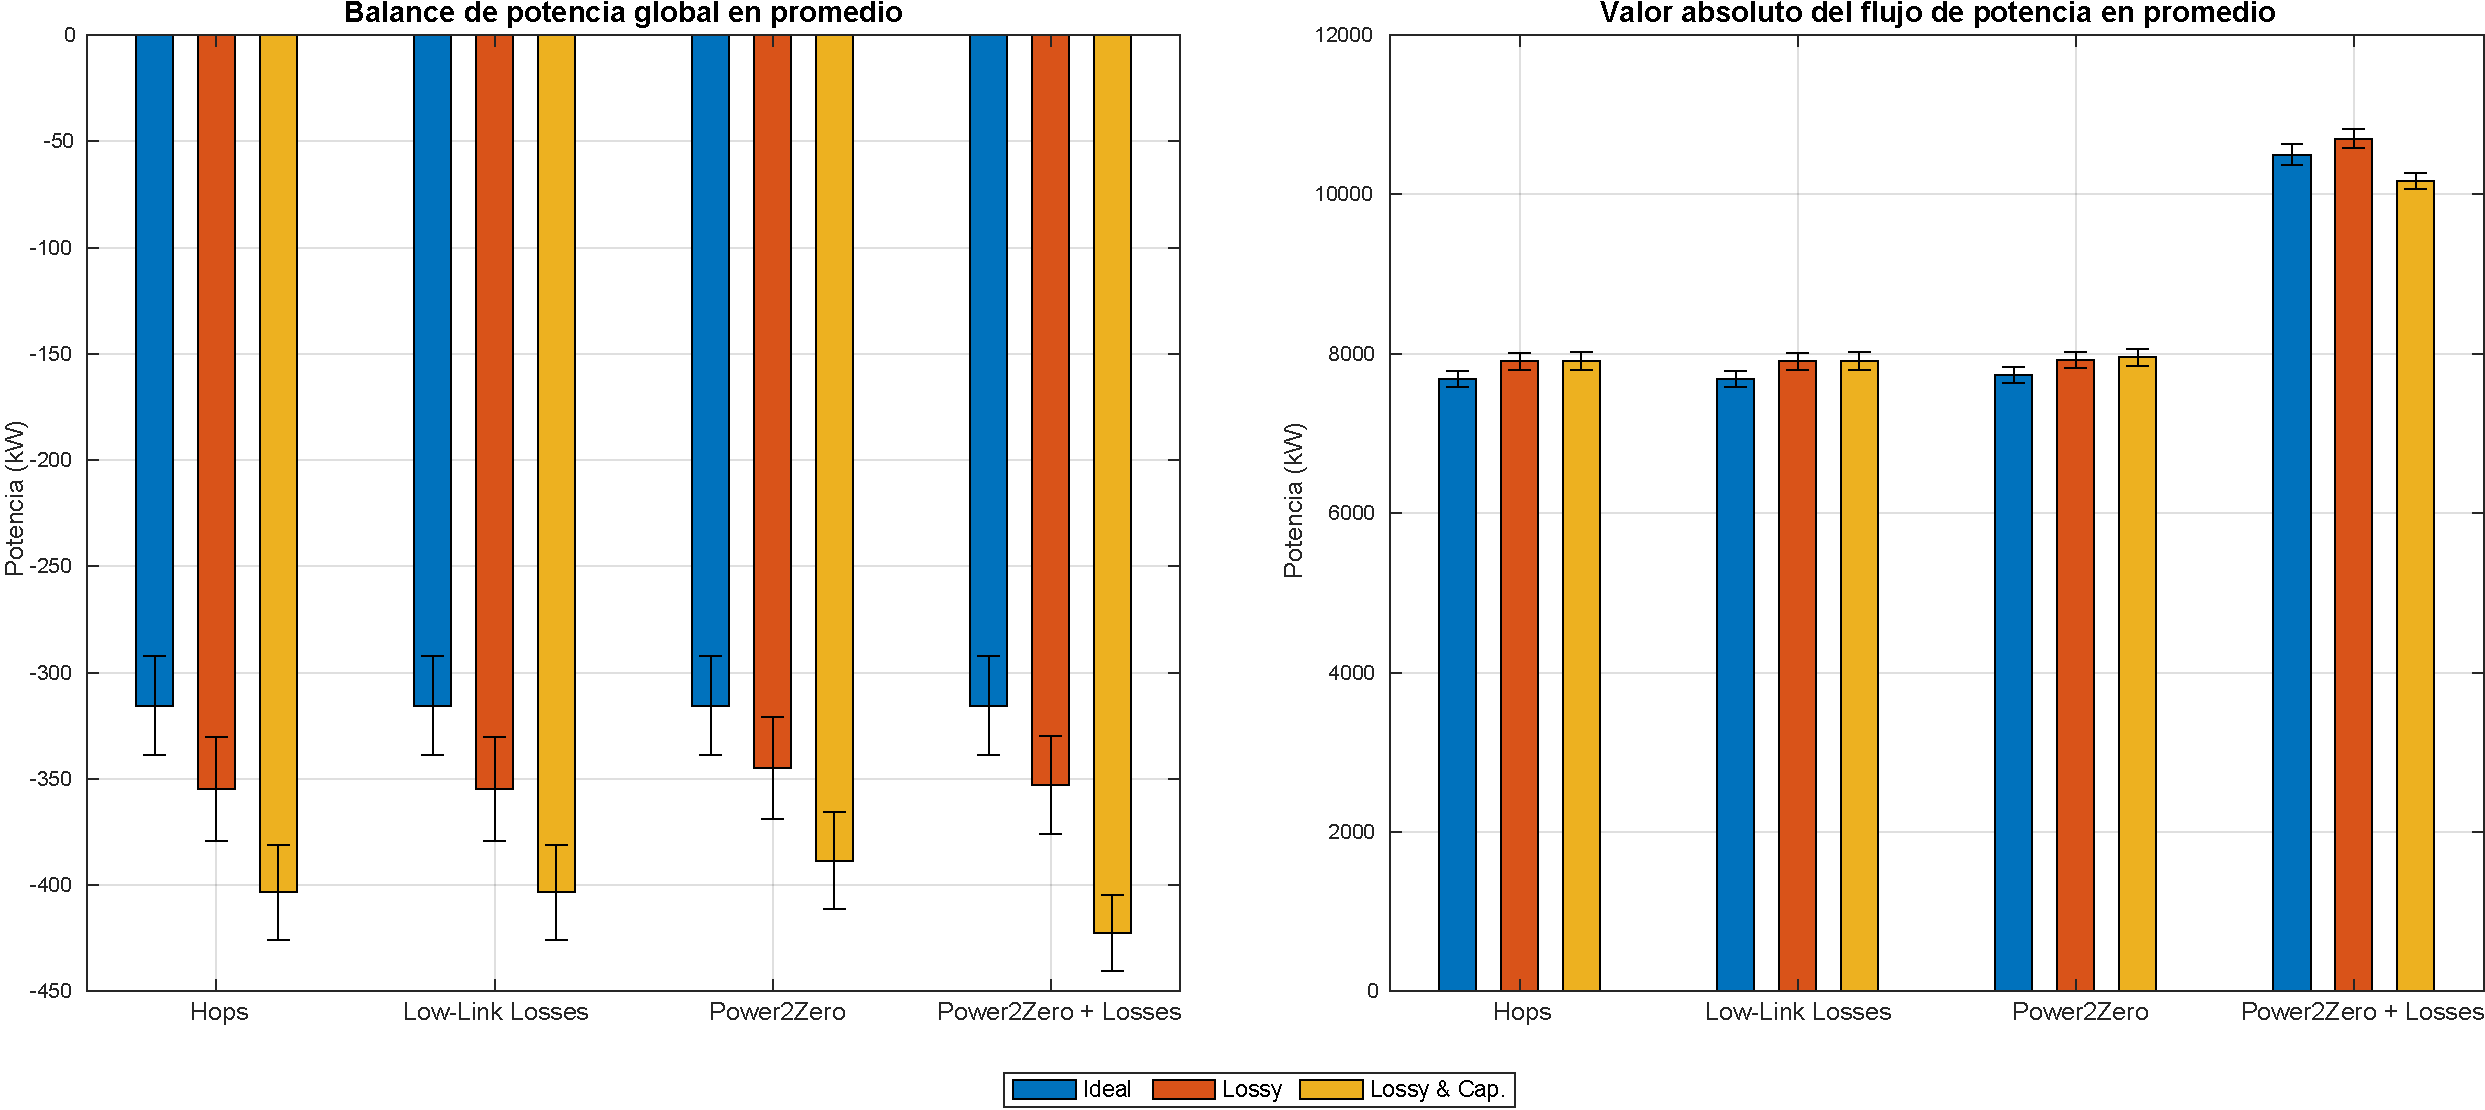
\includegraphics[width=\textwidth]{fig/07_bloste/bloste_08.pdf}
    \caption{Balance de potencia global en promedio y valor absoluto del flujo de potencia - Resultados base.}
    \label{fig:fig_base_global_powers}
\end{figure*}

La Figura~\ref{fig:fig_base_global_powers} muestra los resultados del balance de potencia considerando los tres escenarios previamente mencionados (Ideal, Con Pérdidas y Con Pérdidas y Restricciones de Capacidad), así como los cuatro criterios de ejemplo descritos en la Sección~\ref{subsec:criteria} (\textit{Hops}, \textit{Low-Link Losses}, \textit{Power2Zero} y \textit{Power2Zero + Losses}, respectivamente). Al analizar la Figura~\ref{fig:fig_base_global_powers}, se observa que, en el escenario ideal, el resultado promedio entre todos los criterios se mantiene constante. Esto era de esperar, dado que no existen pérdidas de transmisión en los enlaces ni limitaciones de capacidad. Como se explicó anteriormente, el resultado en este escenario corresponde a la suma de todas las configuraciones de carga de los nodos de la topología, independientemente de las rutas de encaminamiento de potencia seleccionadas. \\
\\
En contraste, al considerar el escenario que incluye tanto pérdidas como restricciones de capacidad, comienzan a apreciarse diferencias significativas. Por ejemplo, el criterio basado en saltos y el criterio de bajas pérdidas en enlaces presentan un comportamiento muy similar. Esta similitud se explica porque, en promedio, las rutas que tienden a seleccionar son independientes de la configuración específica de carga en un instante de tiempo determinado, y se basan principalmente en características intrínsecas de la ruta, como el número de saltos o las pérdidas acumuladas a lo largo del camino.  Entre todos los criterios, el de balance de potencia local a cero (\textit{power2zero}) muestra el mejor desempeño. Como se discutió previamente, este criterio busca, en última instancia, la ruta que, en un solo paso, acerca el balance local de potencia lo más posible a cero. Por ello, incluso en un modelo influenciado por pérdidas, este enfoque optimiza indirectamente el balance global de potencia al fomentar la auto-compensación local entre los nodos. Sin embargo, el criterio \textit{power2zero} con pérdidas presenta un desempeño menor, ya que su función de coste, que originalmente hereda del criterio estándar \textit{power2zero}, se ve afectada negativamente por la presencia de pérdidas de potencia.\\
\\
Asimismo, en la Figura~\ref{fig:fig_base_global_powers} se analiza el valor absoluto del flujo de potencia, el cual refleja la cantidad total de energía transferida a lo largo de la topología. En promedio, los tres primeros criterios muestran la misma transferencia absoluta de potencia. No obstante, el criterio \textit{Power2Zero} con pérdidas exhibe un mayor volumen de potencia transferida. Este comportamiento se debe a que, en términos relativos, dicho criterio requiere un mayor número de iteraciones para converger, como se ilustrará más adelante en la Figura~\ref{fig:fig_base_global_time_iter}.


\begin{figure*}[ht!]
    \centering
    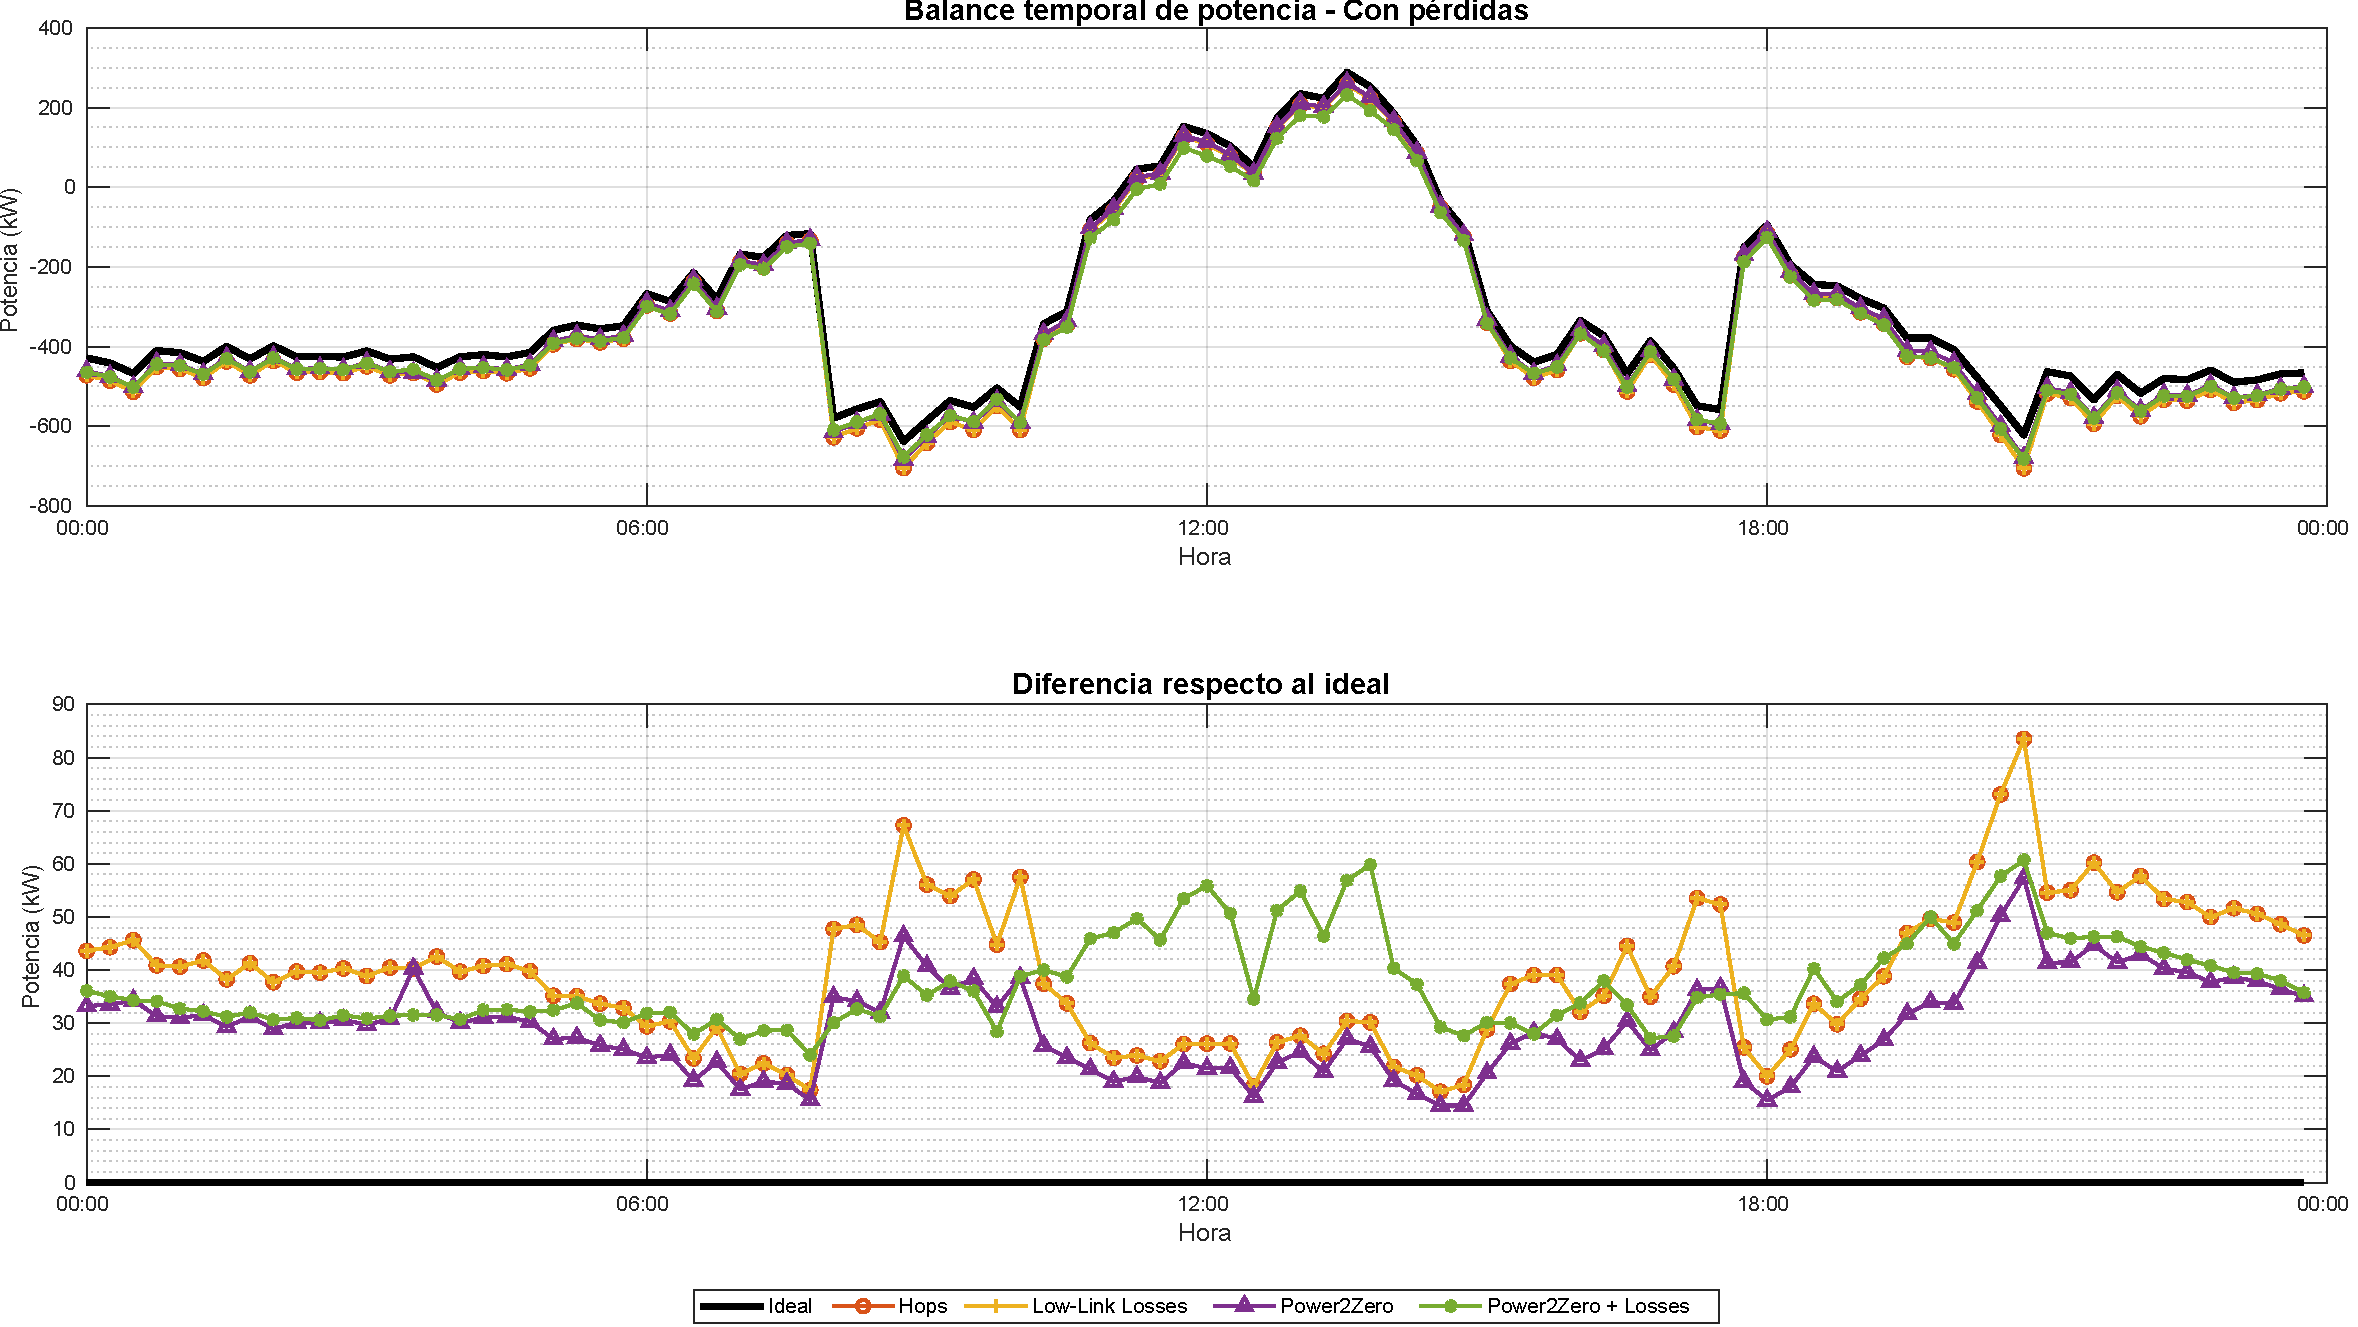
\includegraphics[width=\textwidth]{fig/07_bloste/bloste_09.pdf}
    \caption{Balance temporal de la potencia global en el escenario con pérdidas - Resultados base.}
    \label{fig:powerBalance_Lossy}
\end{figure*}

Continuando con las Figuras~\ref{fig:powerBalance_Lossy} y~\ref{fig:fig_base_TempPowerBalance_LossyCap}, se analiza la evolución temporal del balance global de potencia en los escenarios que consideran pérdidas, y tanto pérdidas como restricciones de capacidad, respectivamente. Estas figuras representan temporalmente el balance global de potencia en el nodo raíz en cada intervalo delta, es decir, cada 15 minutos. Por lo tanto, puede observarse una analogía con el comportamiento en el entorno real, como se ilustró previamente en la Figura~\ref{fig:loads_global_view}.\\
\\
Por ello, las figuras muestran las desviaciones de estos balances respecto al escenario base, correspondiente al caso ideal. Esta representación fue necesaria debido a la homogeneidad de los resultados, con el fin de enfatizar de manera más clara las diferencias entre ellos. De ambas figuras se desprende que un criterio se posiciona como el más efectivo para adaptarse a las configuraciones dinámicas de carga de la topología: el criterio \textit{Power2Zero}. Como se discutió previamente, al priorizar ajustes locales del balance de potencia hacia cero, este criterio minimiza eficazmente las pérdidas y mitiga la degradación del balance global de potencia. Esto ocurre porque el algoritmo fomenta que los nodos se auto-compensen localmente, reduciendo la necesidad de suministro externo de energía.

\begin{figure*}[ht!]
    \centering
    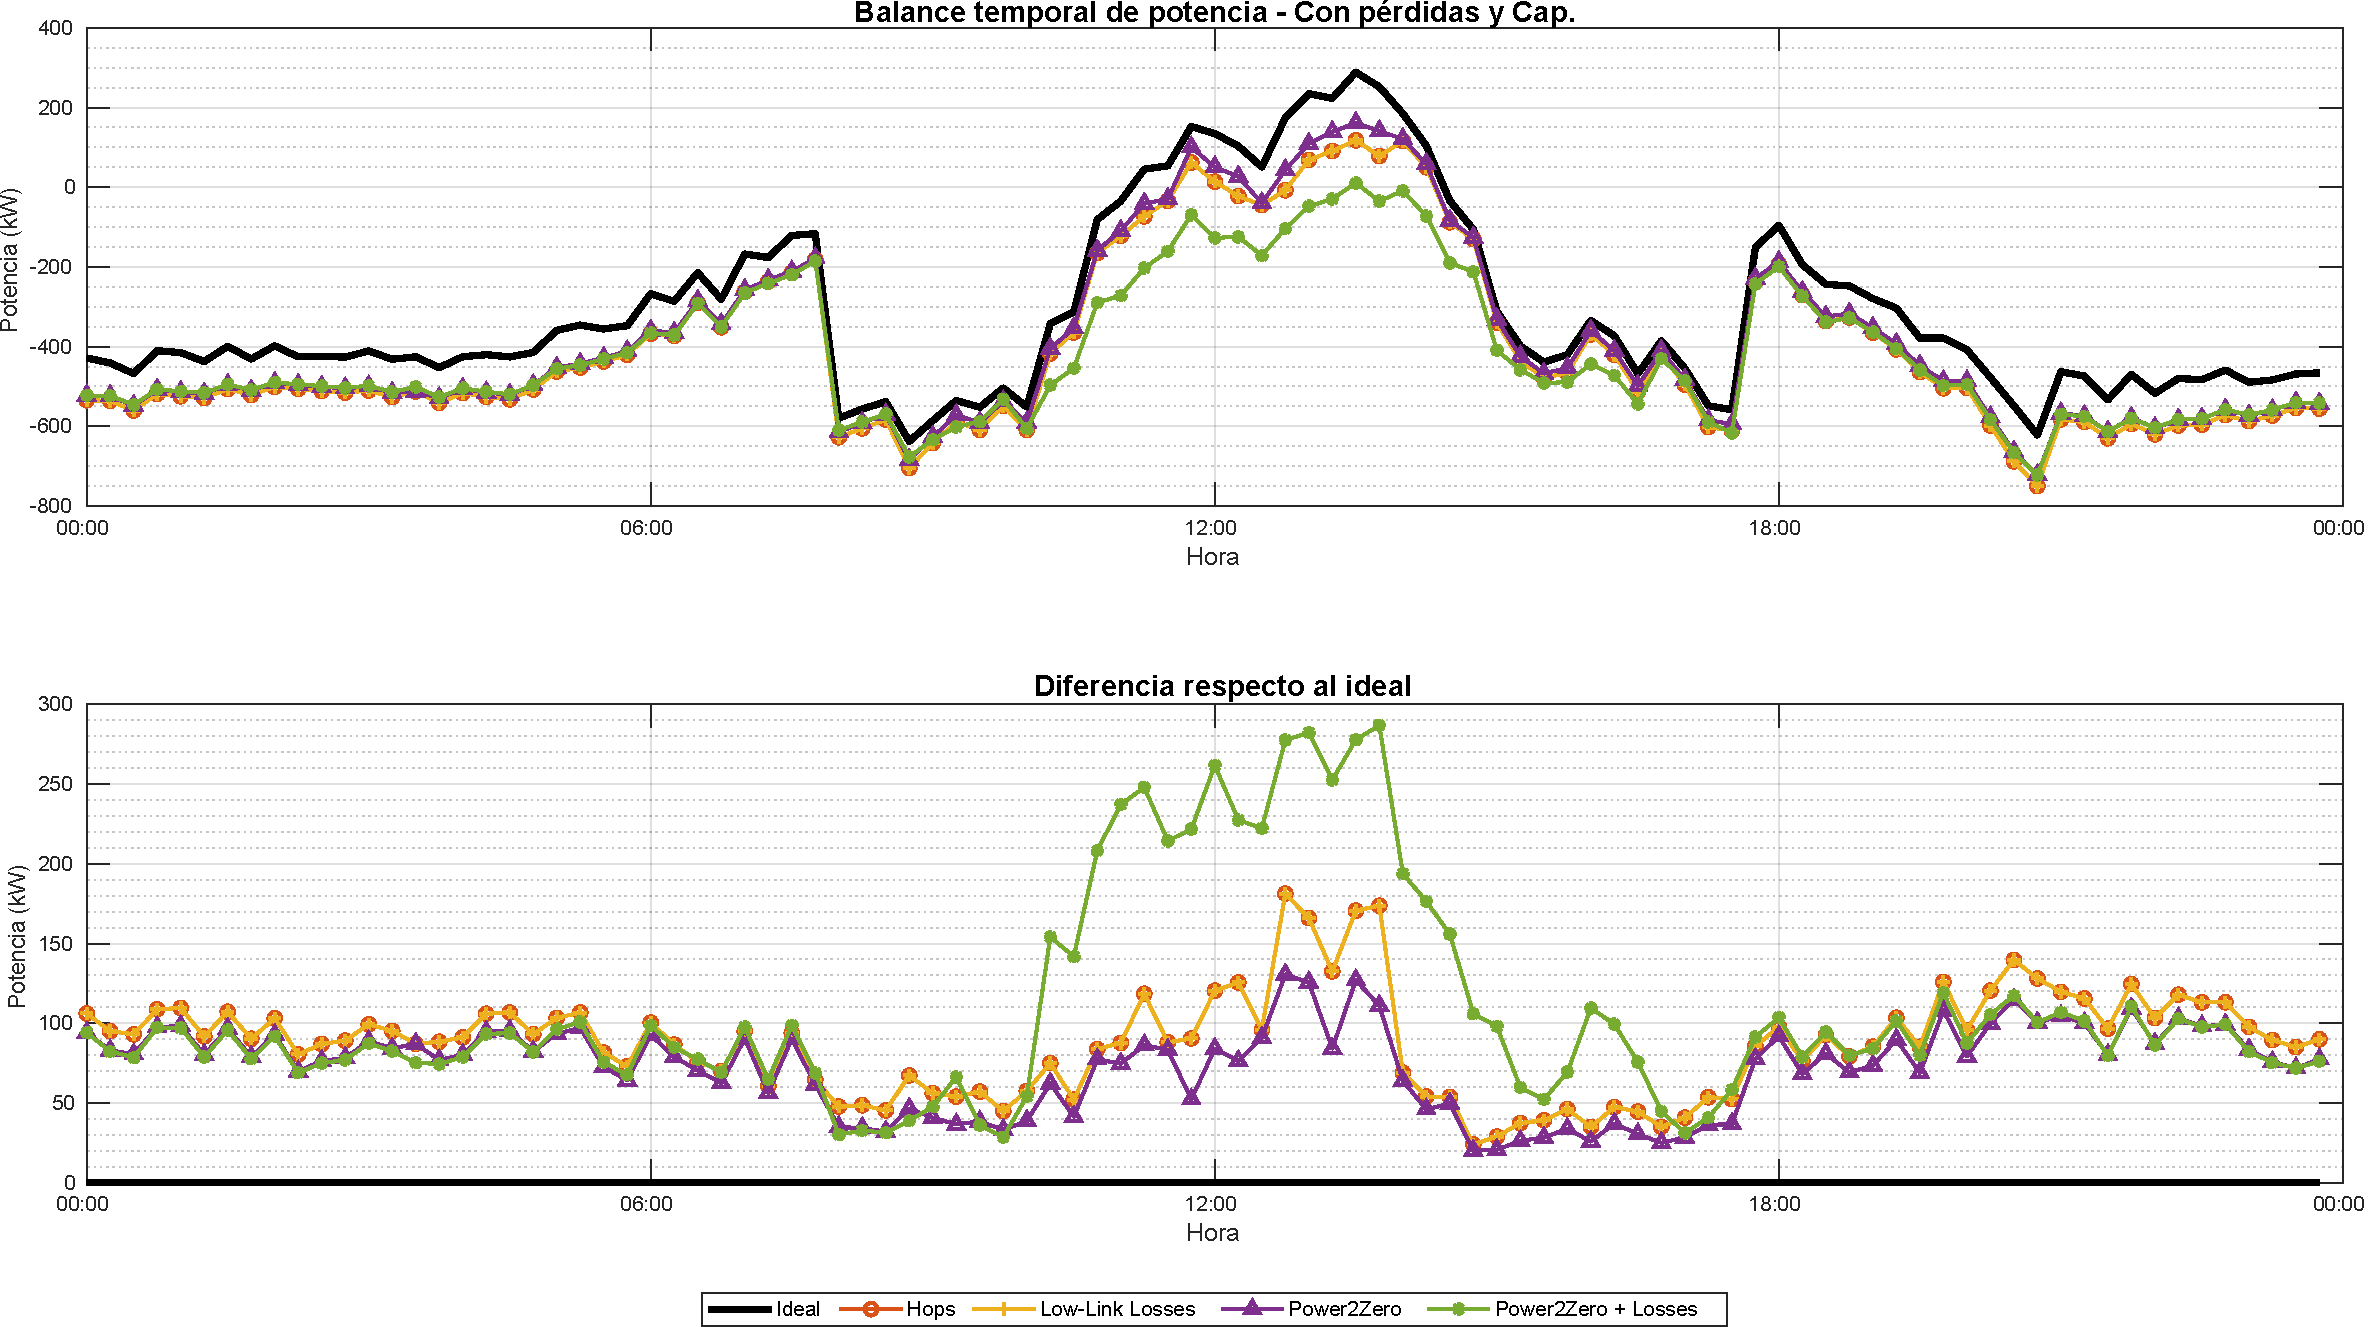
\includegraphics[width=\textwidth]{fig/07_bloste/bloste_10.pdf}
    \caption{Balance temporal de la potencia global en el escenario con pérdidas y capacidades - Resultados base.}
    \label{fig:fig_base_TempPowerBalance_LossyCap}
\end{figure*}


En contraste, el criterio basado en saltos y el criterio de bajas pérdidas en enlaces presentan un comportamiento más homogéneo. Esto se debe directamente a sus respectivas funciones de coste, que priorizan la selección de rutas en función de características intrínsecas de la topología, más que de las variaciones dinámicas en las configuraciones de carga. Como resultado, estos criterios permanecen en gran medida indiferentes a las fluctuaciones temporales de demanda y generación dentro de la topología. Cabe destacar que, como se observa en la Figura~\ref{fig:powerBalance_Lossy}, el criterio \textit{Power2Zero + Losses} representa un compromiso entre los criterios basados en saltos y bajas pérdidas en enlaces. Su comportamiento es más moderado en comparación con estos dos criterios, aunque no alcanza completamente el nivel de optimización logrado por \textit{Power2Zero}.\\
\\
Los últimos parámetros analizados en los resultados base son el tiempo total de convergencia y el número de iteraciones requeridas por cada criterio para alcanzar la convergencia en el enfoque iterativo descrito en la Subsección~\ref{subsec:iterativeBalance}. Se define convergencia como el estado en el que no persisten desequilibrios de potencia residuales dentro de la topología. Como se ilustra en la Figura~\ref{fig:fig_base_global_time_iter}, el criterio con el menor tiempo de convergencia es el criterio basado en saltos. Este resultado es esperable, dado que su función de coste se basa únicamente en contabilizar la longitud de las etiquetas difundidas. En consecuencia, converge en promedio en una sola iteración. Un patrón similar se observa para el criterio de bajas pérdidas en enlaces, que sigue un enfoque análogo al del criterio basado en saltos.  Sin embargo, a pesar de requerir en promedio únicamente una iteración, el criterio de bajas pérdidas en enlaces presenta el mayor tiempo total de convergencia. Esto se debe a la mayor complejidad computacional asociada a su función de coste, que evalúa todas las características intrínsecas de toda la ruta, en lugar de apoyarse en un cálculo a un solo salto.

\begin{figure*}[ht!]
    \centering
    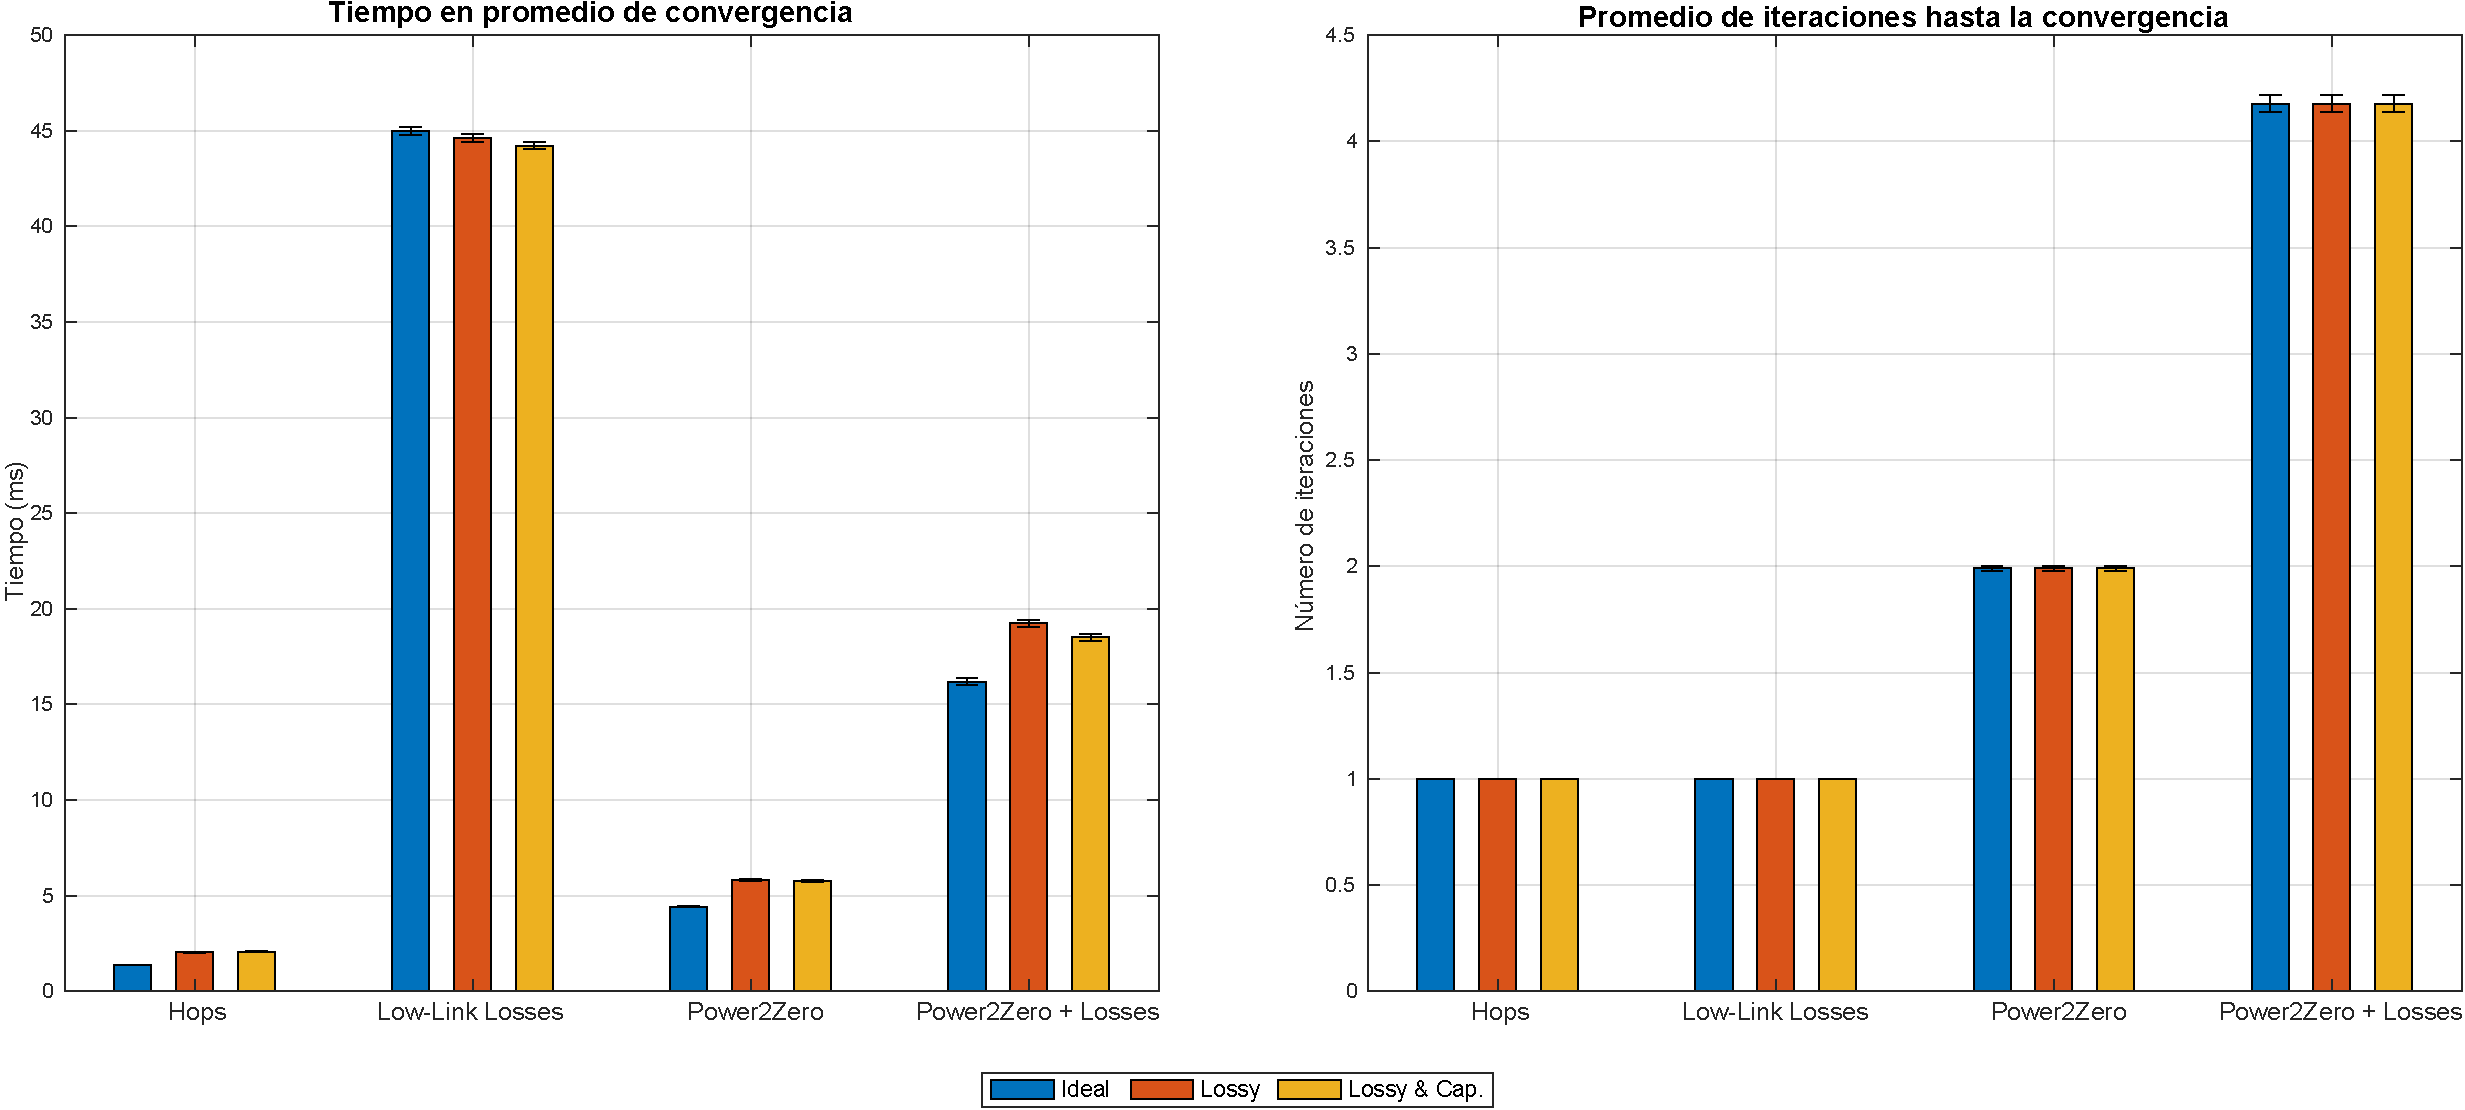
\includegraphics[width=\textwidth]{fig/07_bloste/bloste_11.pdf}
    \caption{Promedio de tiempo/iteraciones hasta la convergencia - Resultados base.}
    \label{fig:fig_base_global_time_iter}
\end{figure*}


Al comparar estos resultados con los dos criterios \textit{Power2Zero}, surge una observación clave: a pesar de requerir, en promedio, el doble o incluso más del doble de iteraciones que los criterios basados en saltos y bajas pérdidas, el tiempo total de convergencia de \textit{Power2Zero} es significativamente menor, alcanzando incluso la mitad del tiempo de convergencia del criterio de bajas pérdidas. Esta eficiencia se debe a que la función de coste de \textit{Power2Zero} se calcula a nivel local de un solo salto, reduciendo la carga computacional por iteración. Por lo tanto, en términos de tiempo de convergencia, el criterio simple \textit{Power2Zero} se destaca como la opción más efectiva. Aunque requiere ligeramente más iteraciones que el criterio basado en saltos, su desempeño superior en el balance de potencia, tanto en escenarios con pérdidas como en escenarios con pérdidas y restricciones de capacidad, demostrando que es lo suficientemente rápido y dinámicamente adaptable para las necesidades específicas de esta topología y sus configuraciones de carga.


\subsubsection{Resultados \textit{All Roots}}

En el escenario con todos los nodos como posibles raíces, denominado como resultados \textit{All Roots}, se evalúan nuevamente los mismos parámetros analizados en los resultados base, no solo como un promedio temporal sobre los 96 intervalos de tiempo, sino también como un promedio agregado de todas las simulaciones en las que distintos nodos actúan como raíz. Como se muestra en las Figuras~\ref{fig:fig_fullrandom_global_powers} y~\ref{fig:fig_fullrandom_global_time_iter}, los resultados relativos al balance global de potencia, al flujo absoluto de potencia, al tiempo de convergencia y al número de iteraciones presentan una notable homogeneidad. Esta consistencia valida la robustez de los criterios evaluados, al demostrar que su desempeño se mantiene en gran medida independiente de la elección del nodo raíz. Además, confirma que el sesgo observado en los resultados base es mínimo.


\begin{figure*}[ht!]
    \centering
    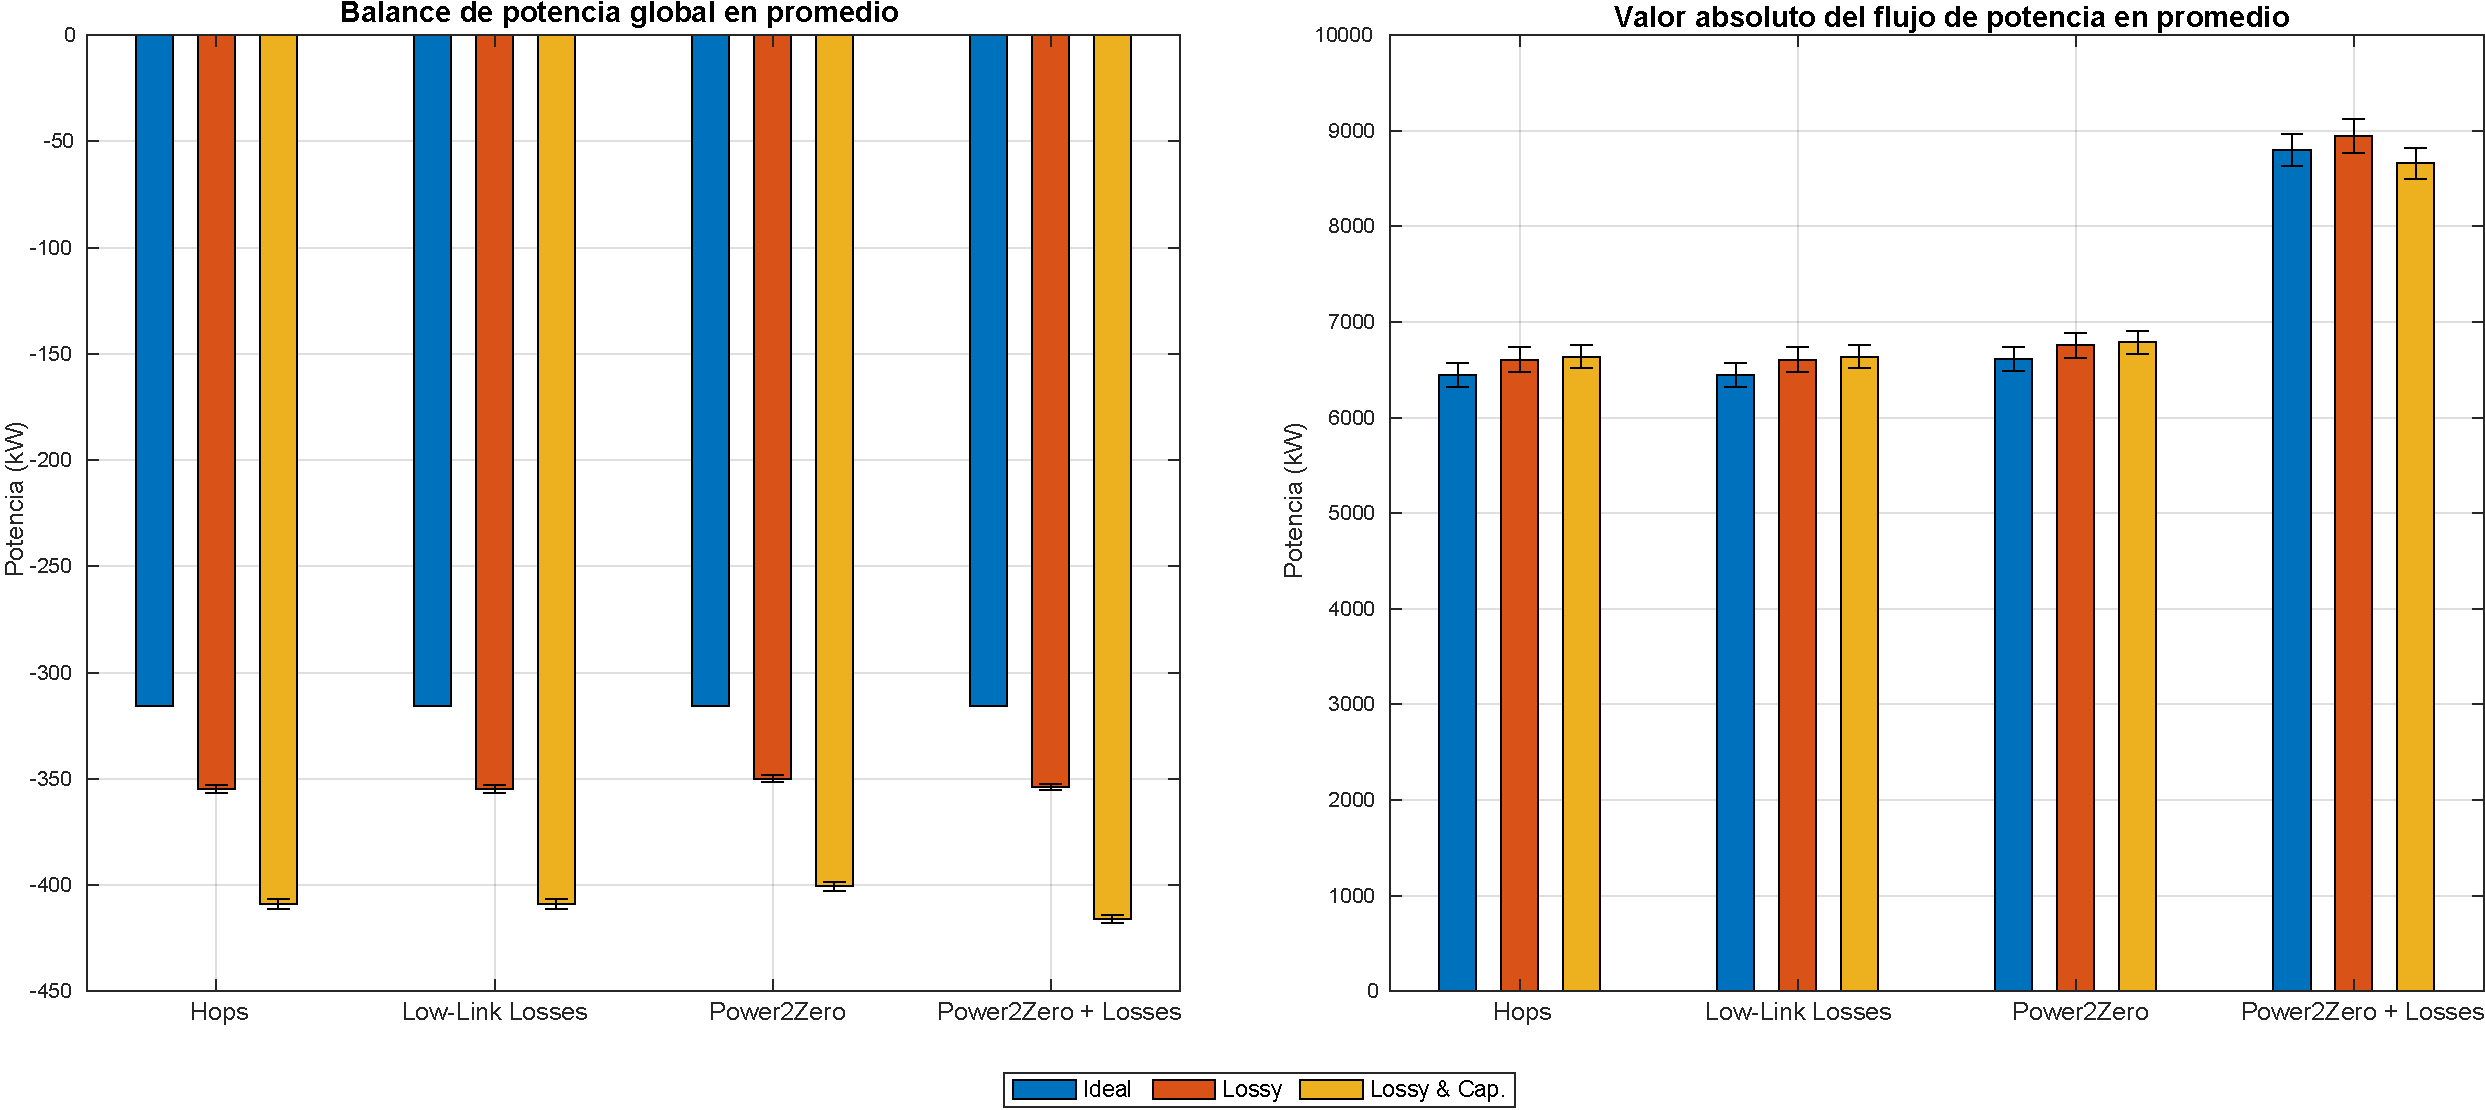
\includegraphics[width=\textwidth]{fig/07_bloste/bloste_12.pdf}
    \caption{Balance de potencia global en promedio y valor absoluto del flujo de potencia - Resultados \textit{All Roots}.}
    \label{fig:fig_fullrandom_global_powers}
\end{figure*}

\begin{figure*}[ht!]
    \centering
    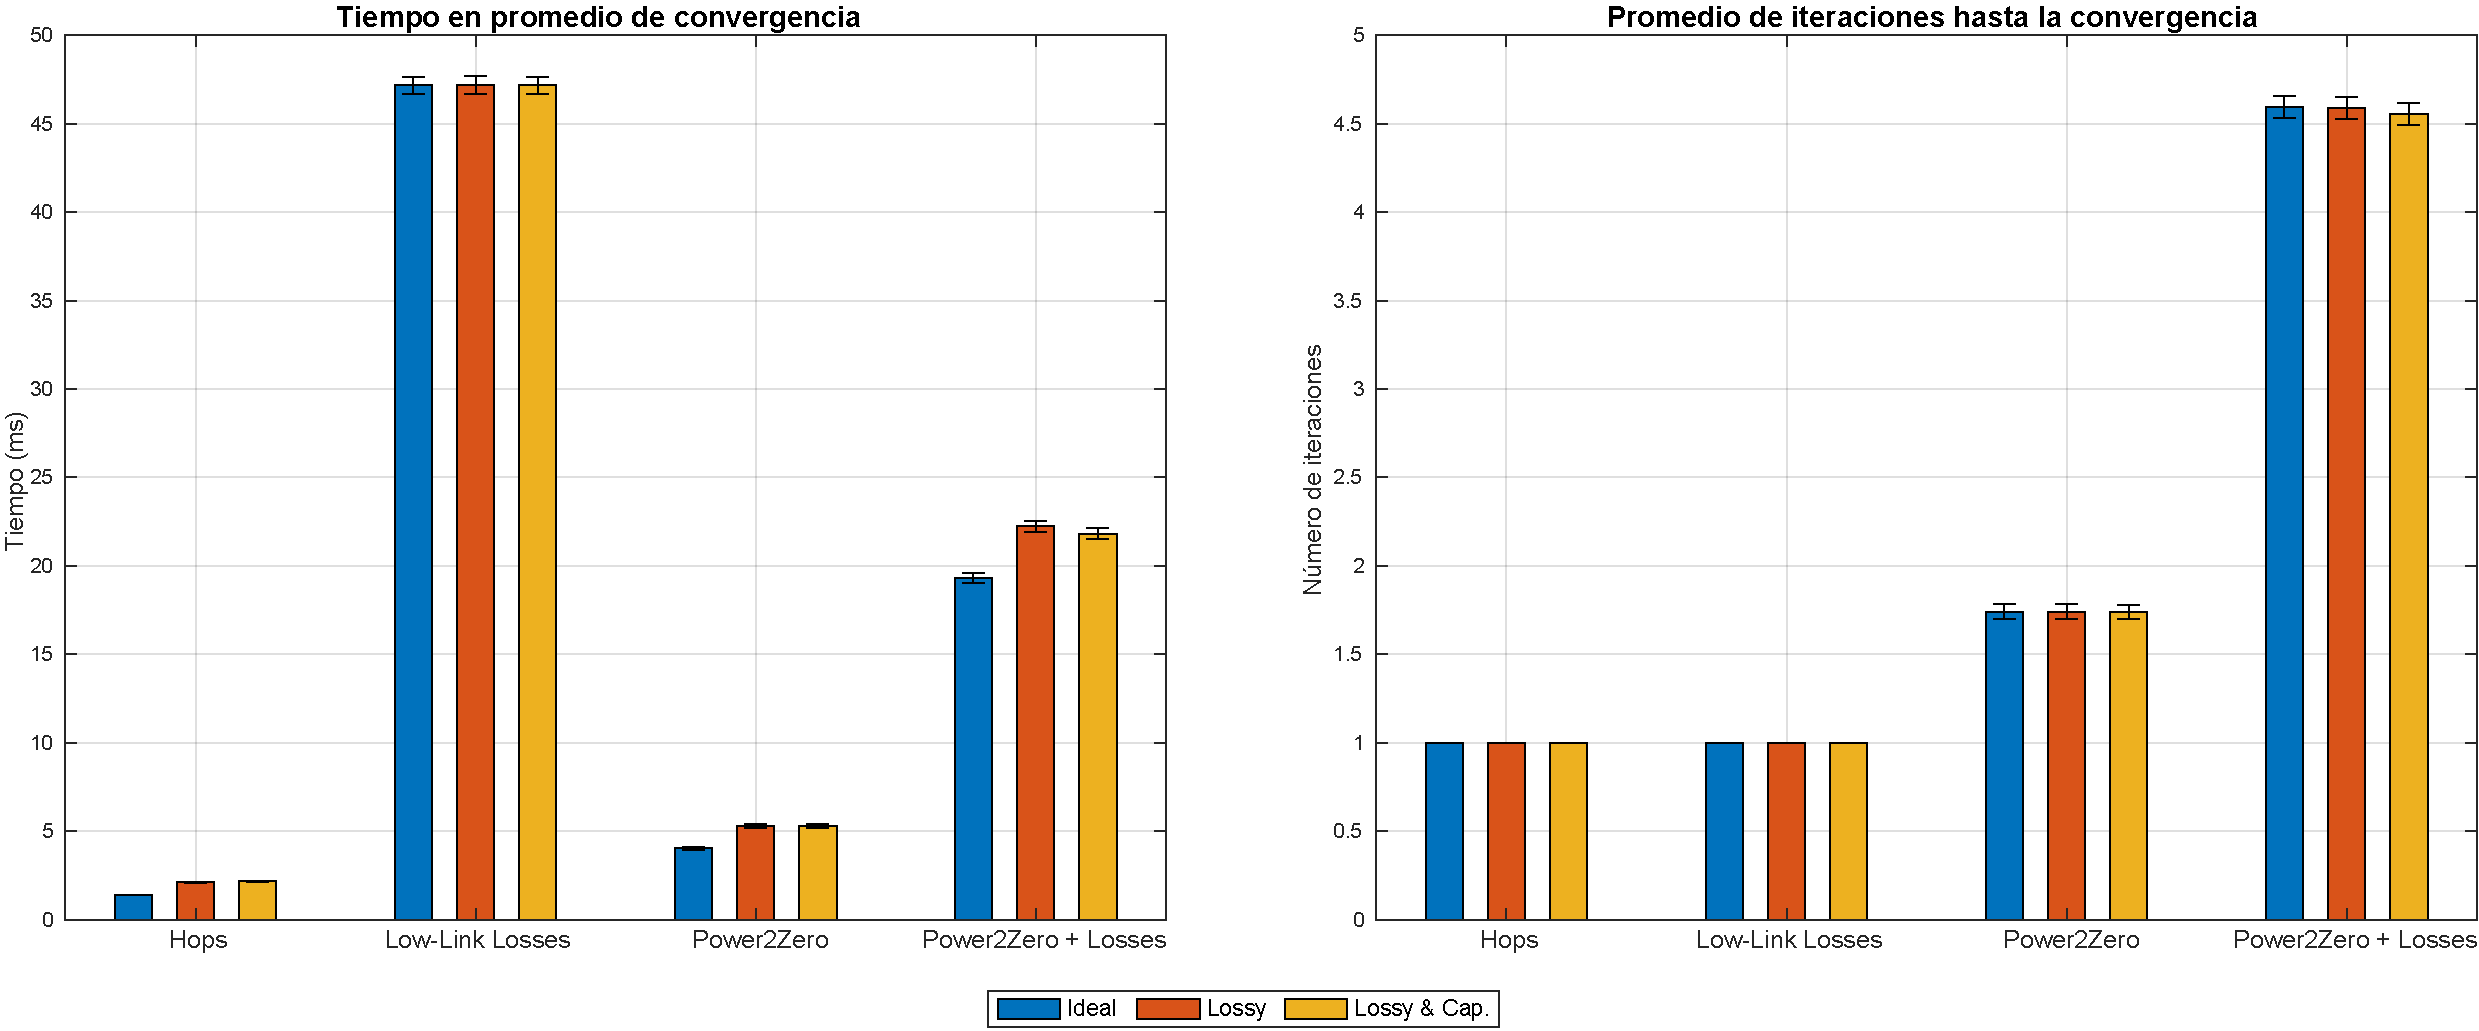
\includegraphics[width=\textwidth]{fig/07_bloste/bloste_13.pdf}
    \caption{Promedio de tiempo/iteraciones hasta la convergencia - Resultados \textit{All Roots}.}
    \label{fig:fig_fullrandom_global_time_iter}
\end{figure*}

Al incrementar el número de simulaciones en diversos escenarios, el intervalo de confianza se ha reducido aún más, reforzando las conclusiones obtenidas en el experimento anterior. En particular, el criterio con mejor desempeño en términos de balance global continúa siendo \textit{Power2Zero}; el criterio que desplaza la mayor cantidad de potencia absoluta es \textit{Power2Zero + Losses}; y el criterio que converge más rápidamente es el basado en saltos, seguido muy de cerca por \textit{Power2Zero}. Estos resultados consolidan a \textit{Power2Zero} como el criterio más efectivo de forma global, al ofrecer un equilibrio óptimo entre rendimiento, velocidad de convergencia y adaptabilidad.\\
\\
Las Figuras~\ref{fig:fig_fullrandom_TempPowerBalance_Lossy} y~\ref{fig:fig_fullrandom_TempPowerBalance_LossyCap} muestran la evolución temporal del balance global de potencia, promediado sobre todas las simulaciones con diferentes nodos raíz en la topología.


\begin{figure*}[ht!]
    \centering
    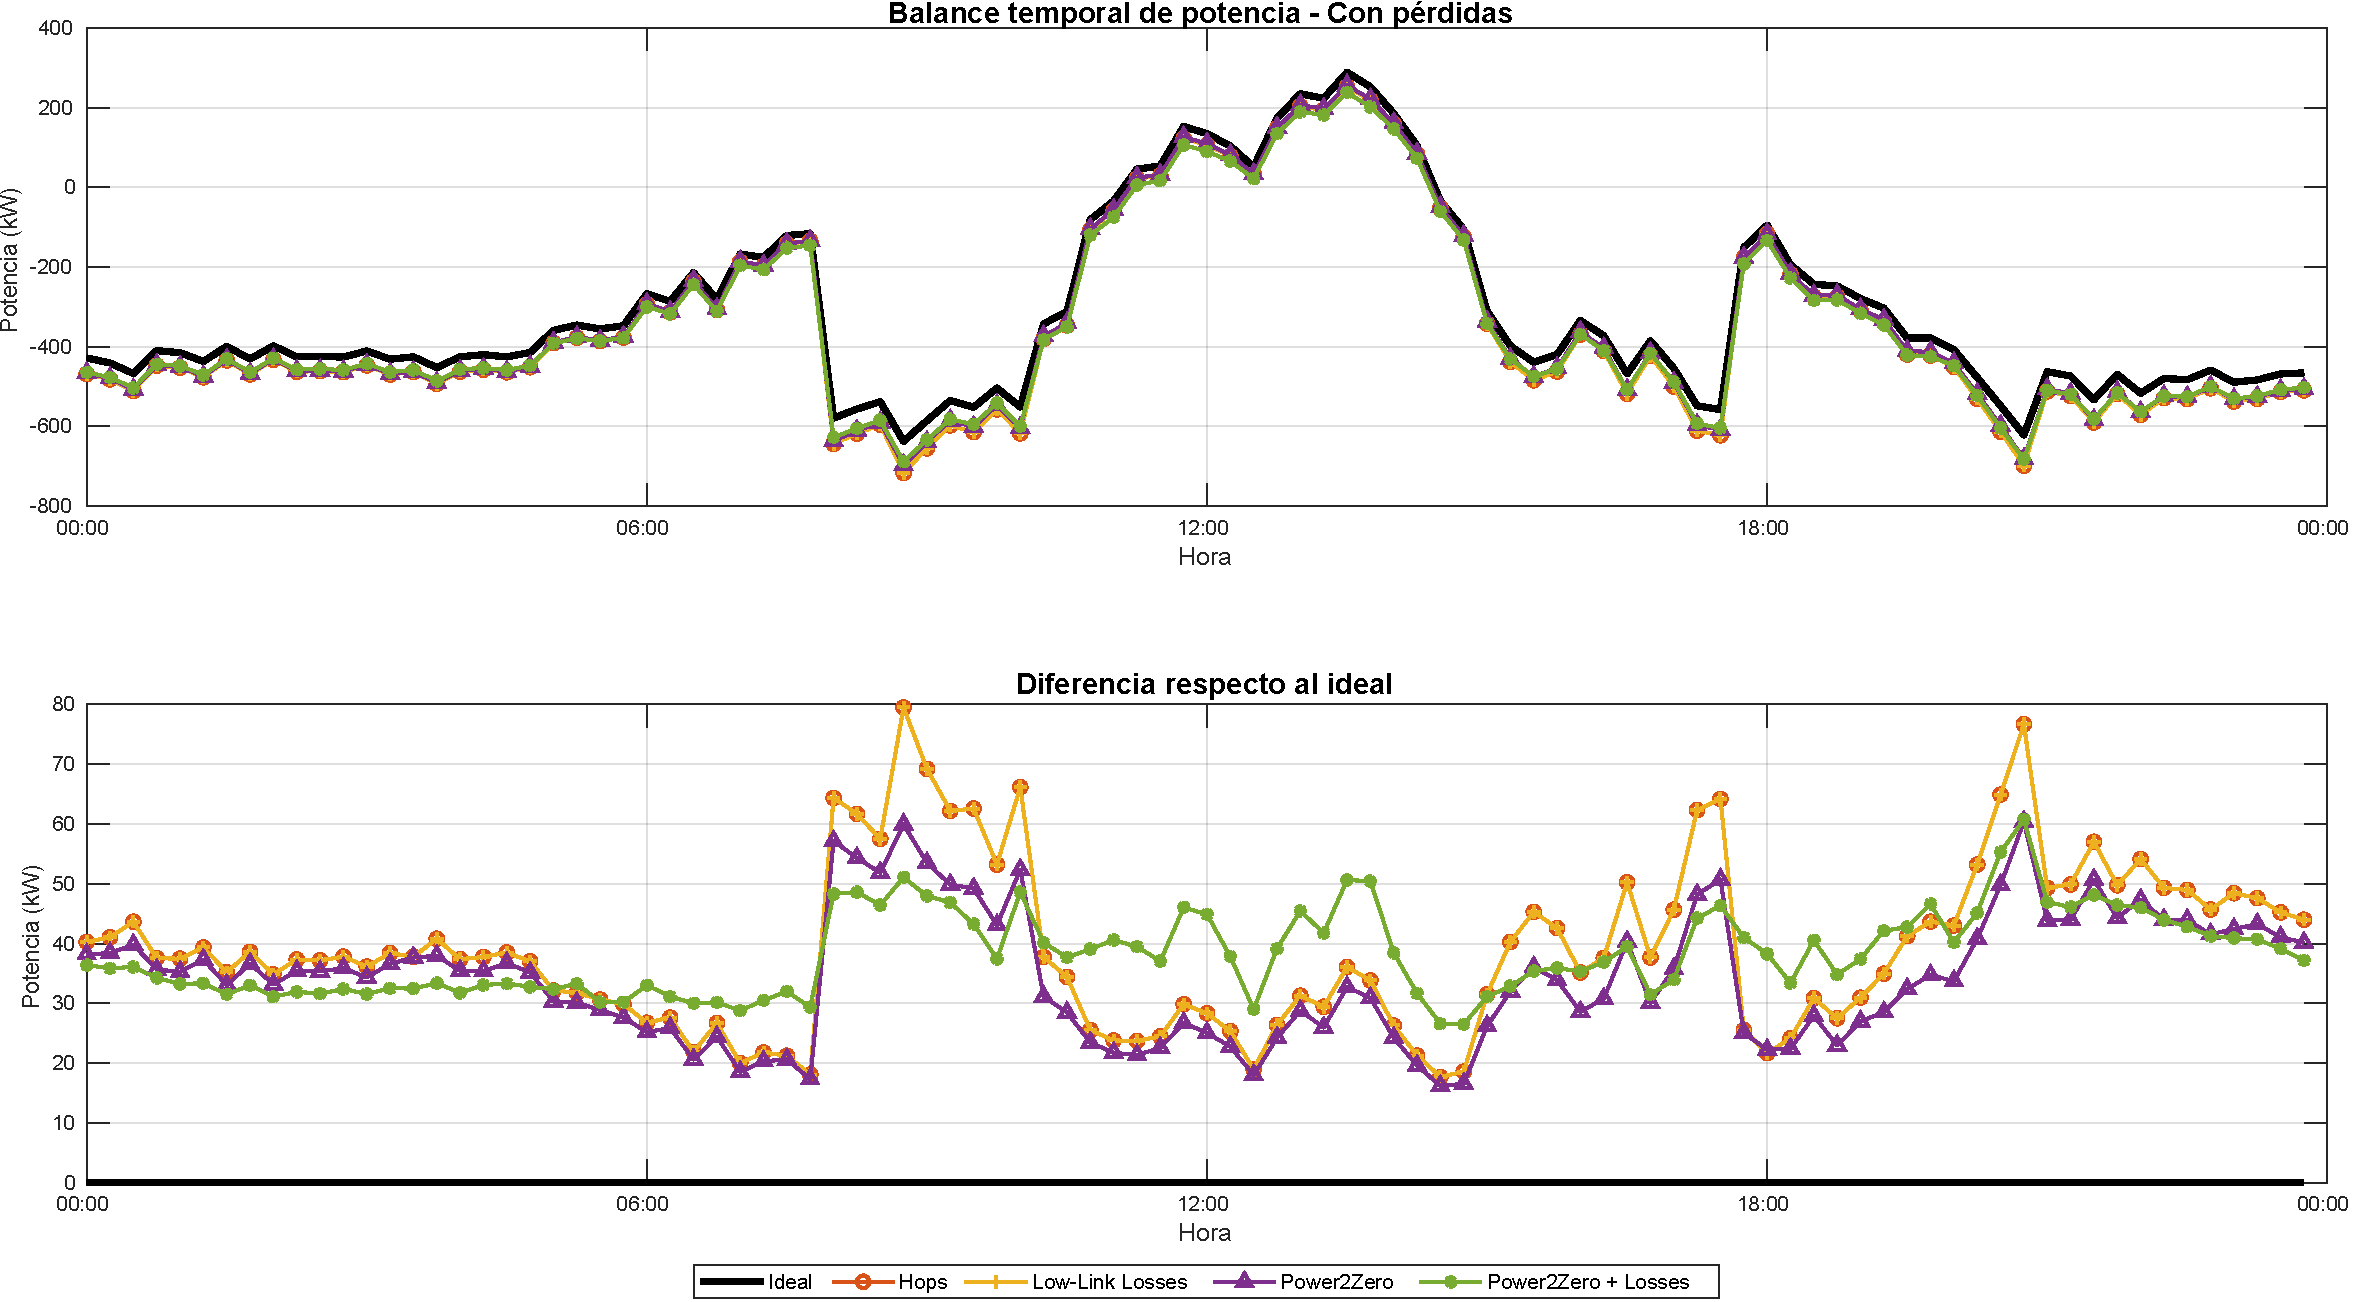
\includegraphics[width=\textwidth]{fig/07_bloste/bloste_14.pdf}
    \caption{Balance temporal de la potencia global en el escenario con pérdidas - Resultados \textit{All Roots}.}
    \label{fig:fig_fullrandom_TempPowerBalance_Lossy}
\end{figure*}

\begin{figure*}[ht!]
    \centering
    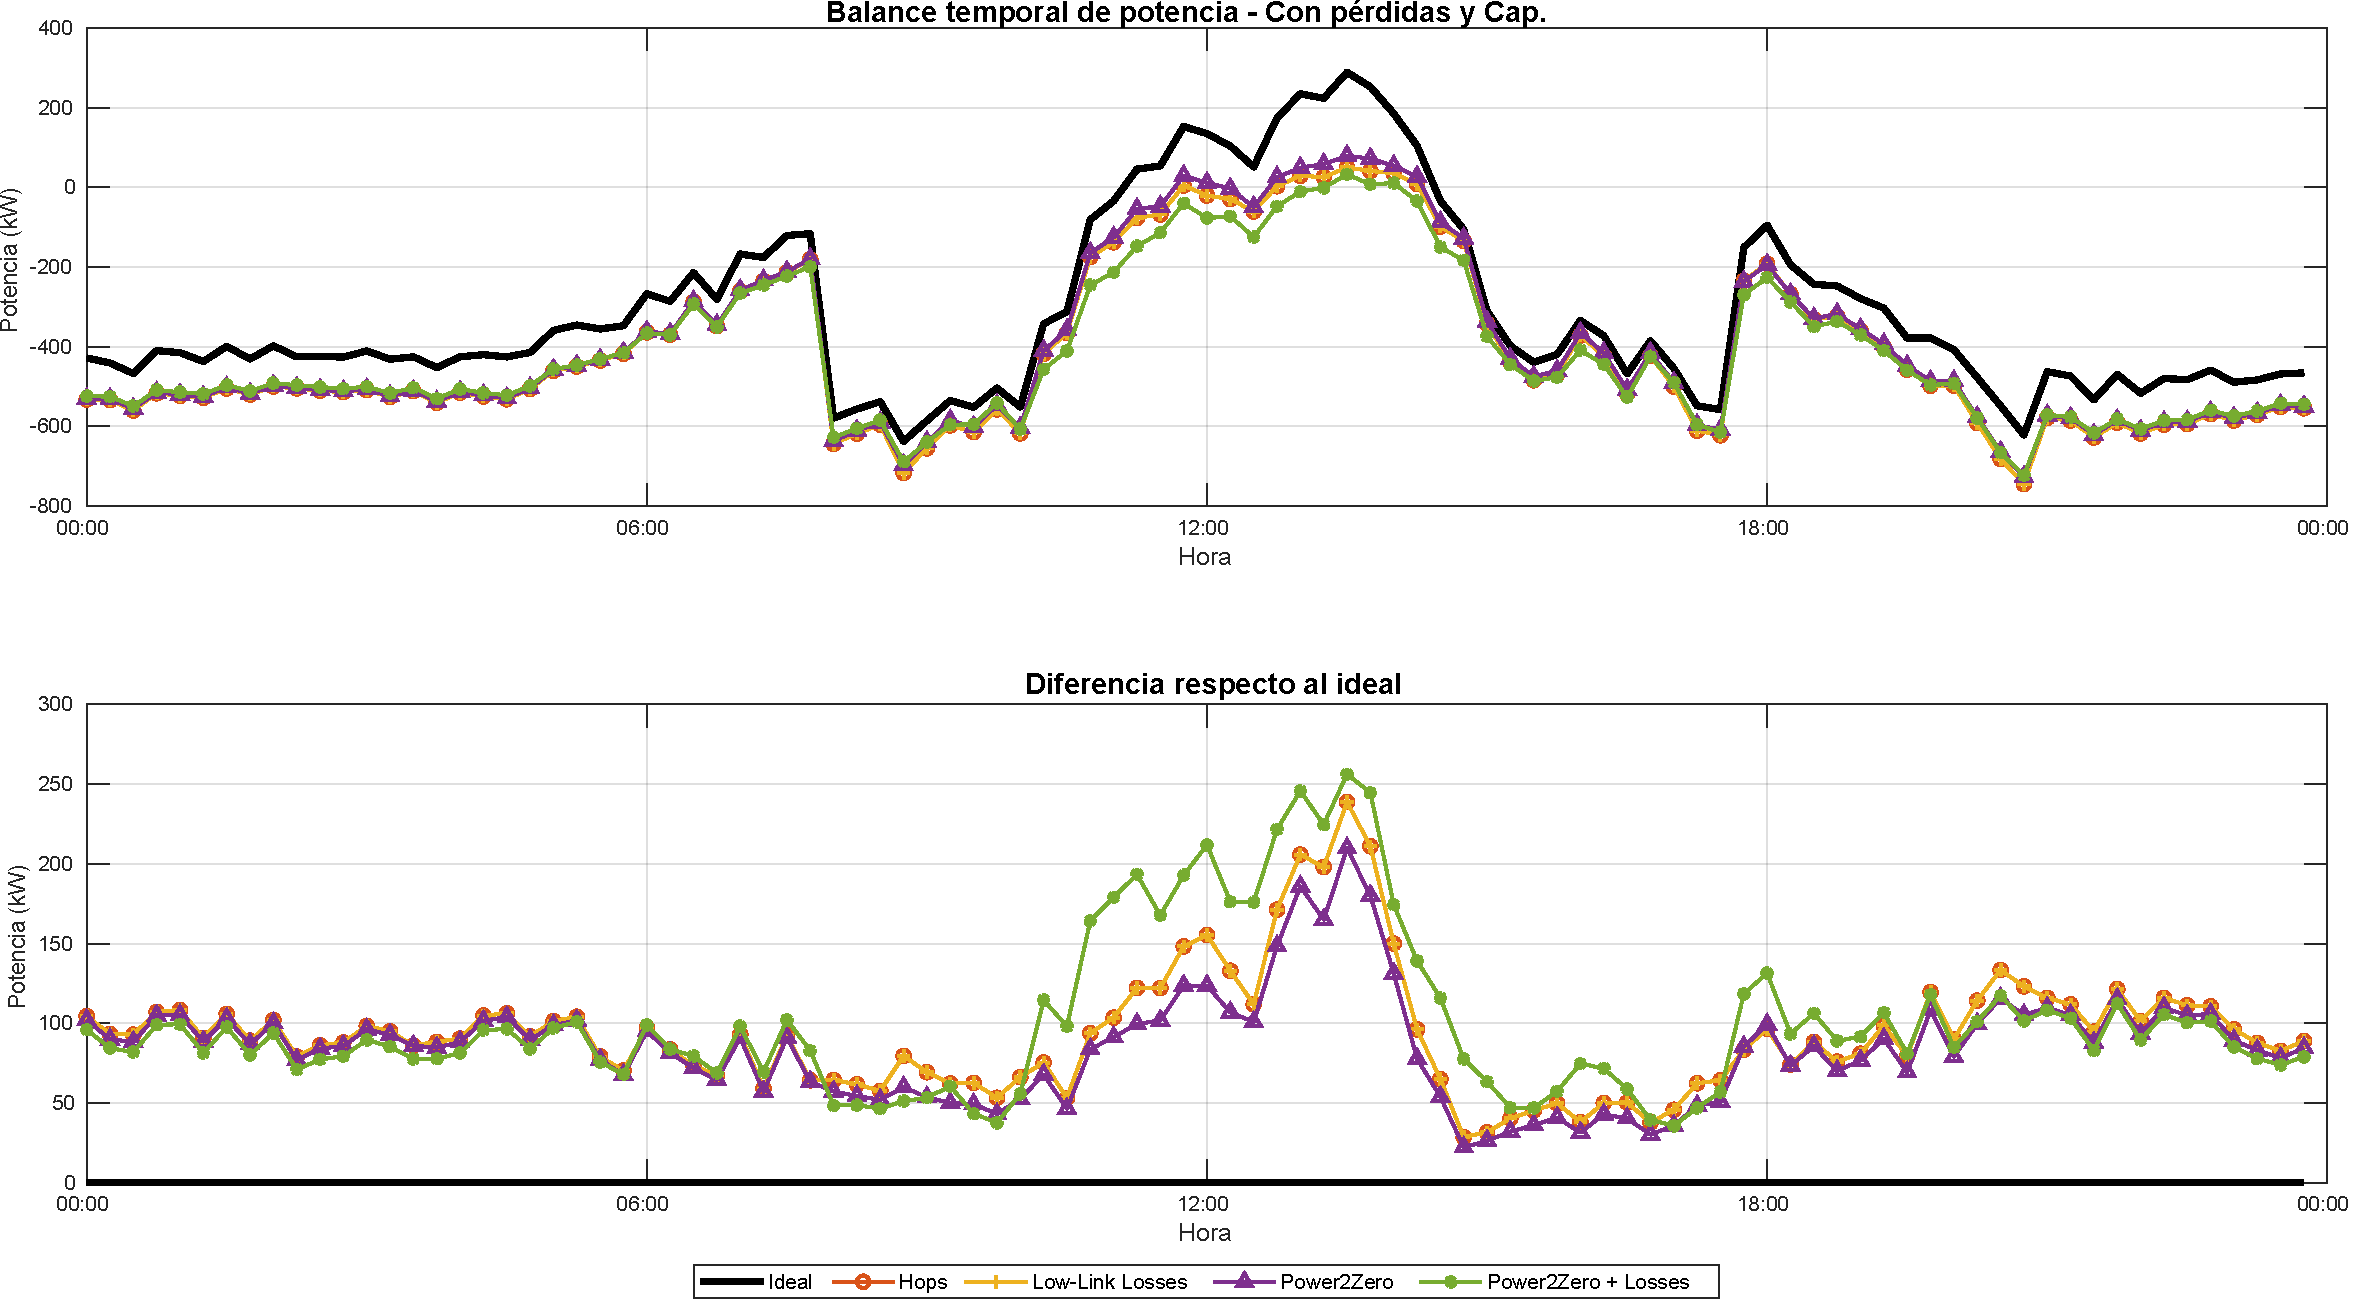
\includegraphics[width=\textwidth]{fig/07_bloste/bloste_15.pdf}
    \caption{Balance temporal de la potencia global en el escenario con pérdidas y capacidades - Resultados \textit{All Roots}.}
    \label{fig:fig_fullrandom_TempPowerBalance_LossyCap}
\end{figure*}

Como era de esperar, los resultados aparecen más suavizados, confirmando las tendencias observadas previamente. El criterio \textit{Power2Zero} continúa mostrando el mejor rendimiento, evidenciando una mayor capacidad de adaptación frente a configuraciones dinámicas de carga. En contraste, los criterios \textit{Hops} y \textit{Low-Link Losses} exhiben un comportamiento más estático, al mantenerse en gran medida inalterados ante las variaciones en la dinámica de distribución de potencia. El criterio \textit{Power2Zero + Losses} se presenta como una solución intermedia, ofreciendo un rendimiento estable y, en ciertos casos, superando incluso a otros enfoques durante los períodos de máxima demanda. Por ejemplo, como se ilustra en la Figura~\ref{fig:fig_fullrandom_TempPowerBalance_Lossy}, se observa que el criterio \textit{Power2Zero}, durante los picos de generación de las 08:00 y las 17:30, logra adaptarse mejor a las nuevas dinámicas de la red, alcanzando un balance de potencia superior ($4.32\%$) en comparación con los criterios basados en número de saltos y en pérdidas. En la misma ventana temporal, el criterio \textit{Power2Zero + Losses} muestra un comportamiento más estático que \textit{Power2Zero} en solitario, llegando incluso a rendir por debajo de los criterios basados en saltos y pérdidas entre las 10:30 y las 15:00. No obstante, este comportamiento más conservador contribuye a una respuesta más uniforme frente a los picos de demanda o generación, tal como se observa antes y después del período principal de generación (08:00–17:30). Estos resultados refuerzan la validación de \textit{Power2Zero} como el criterio más robusto y adaptable para optimizar el balance de potencia en condiciones de red dinámicas.

\subsection{Evaluación sobre la topología IEEE 34-Node Test Feeder}

En aras de evaluar la capacidad de operación del algoritmo en redes de distribución eléctrica diferentes, se ha elegido la topología \gls{ieee} 34-Node Test Feeder. La topología \gls{ieee} 34-bus~\cite{Schneider17} constituye un modelo de referencia ampliamente utilizado en la evaluación de sistemas de distribución eléctrica. Corresponde a un alimentador real, asimétrico y ligeramente cargado, ubicado en Arizona y operando a una tensión nominal de 24,9~kV. Entre sus características principales destacan la presencia de ramales de gran longitud, líneas tanto monofásicas como trifásicas, reguladores de tensión en línea, así como una breve sección operando a 4,16~kV. La Figura~\ref{fig:ieee34} muestra la disposición de la topología \gls{ieee} 34-bus. Como puede observarse, se trata de una estructura prácticamente lineal, con un grado de mallado (\textit{mesh}) muy limitado. Con el fin de permitir una evaluación más representativa de las diferencias entre los distintos criterios analizados, ha sido necesario incorporar enlaces adicionales, representados en color naranja en la Figura~\ref{fig:ieee34}.


\begin{figure}[ht!]
    \centering
    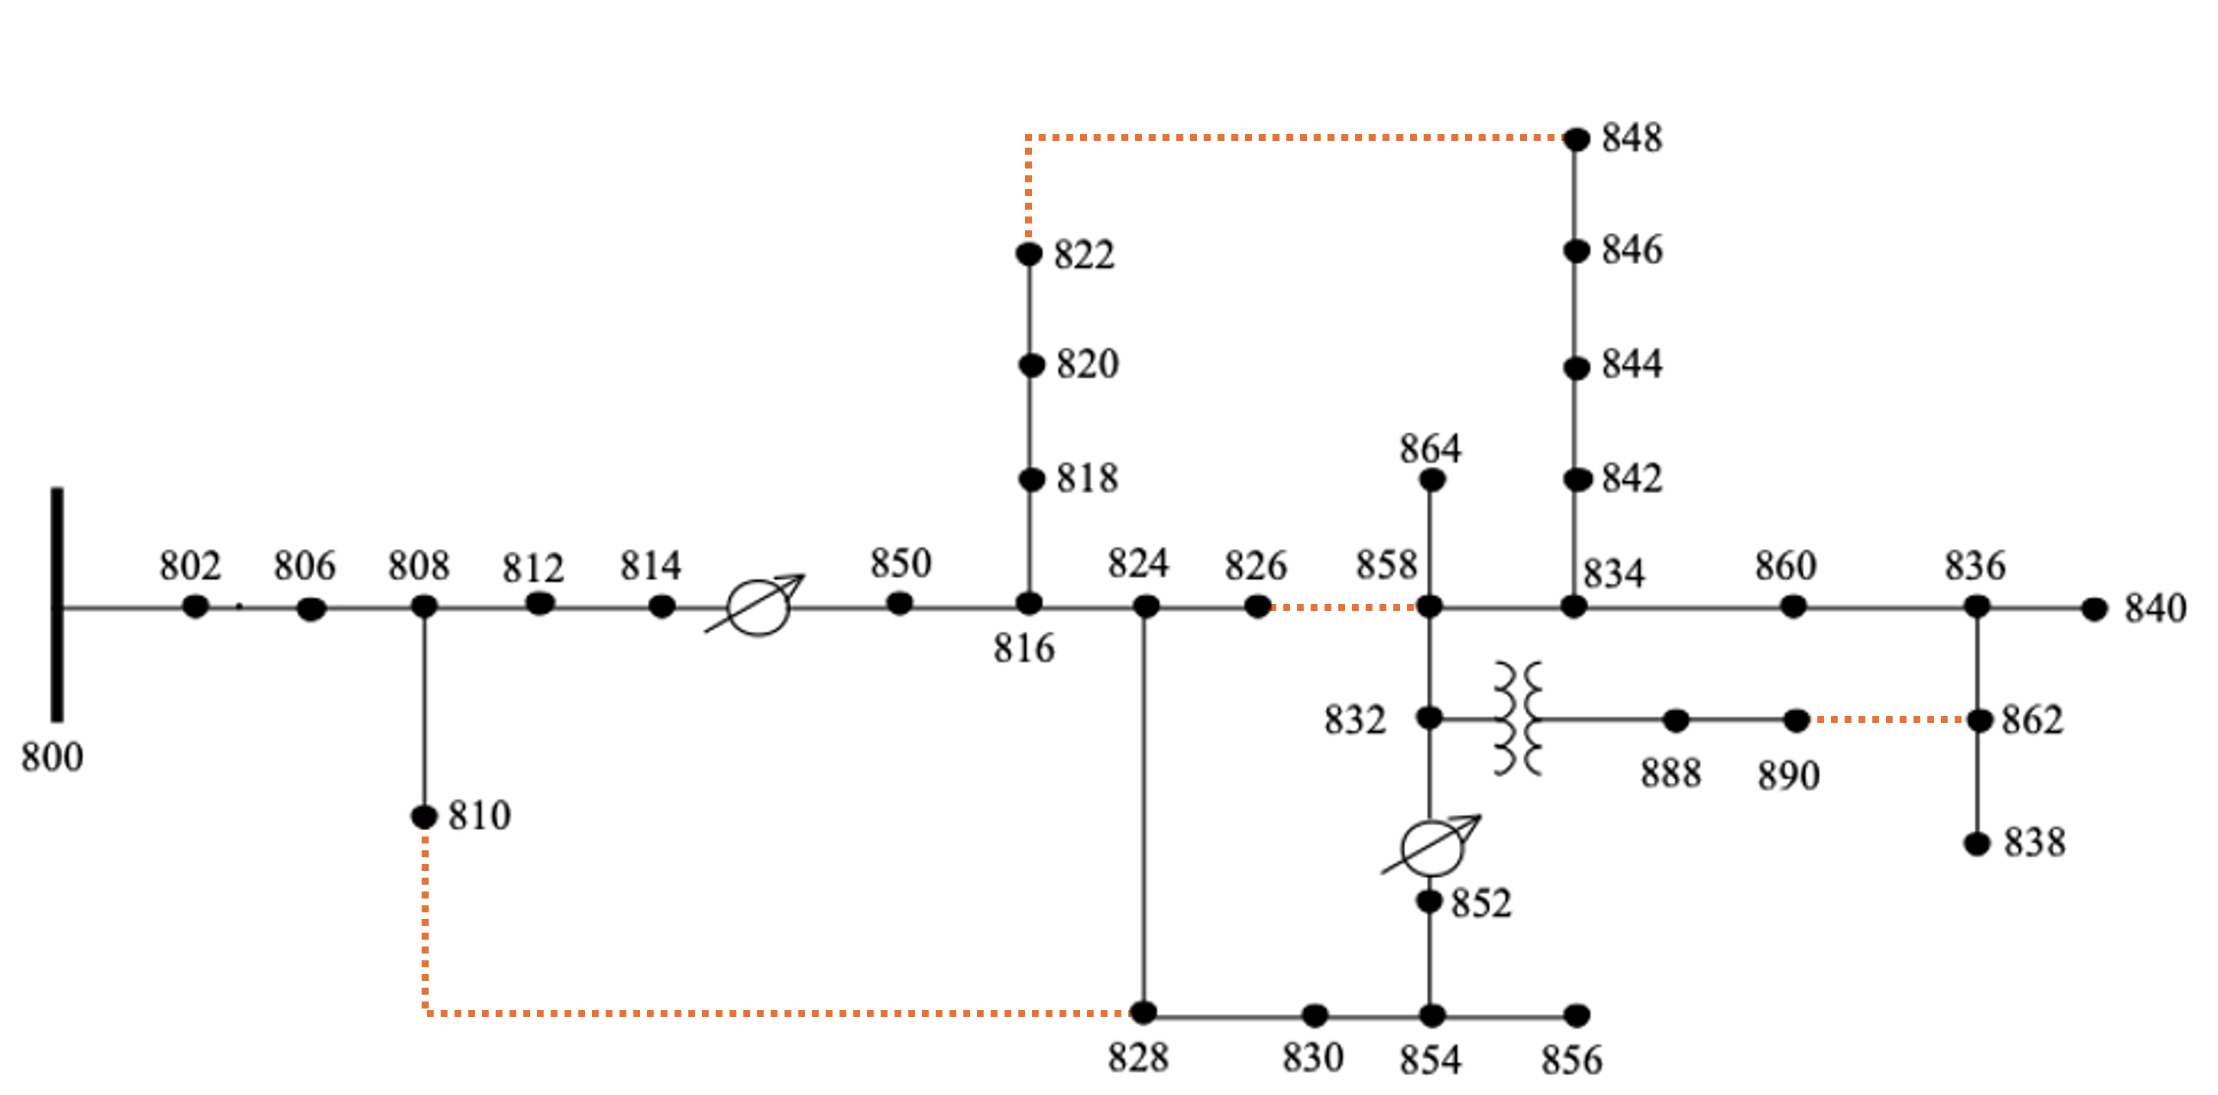
\includegraphics[width=0.7\textwidth]{fig/07_bloste/bloste_16.png}
    \caption{Topología IEEE 34-Node Test Feeder.}
    \label{fig:ieee34}
\end{figure}

Con respecto a la configuración de cargas de la topología, se emplearon también los perfiles de nodo especificados en \cite{Schneider17}. Con el objetivo de garantizar la homogeneidad de las condiciones iniciales de la evaluación llevada a cabo en la topología \gls{ieee} 123-bus, se selecciono de manera aleatoria perfiles de cargas a los 34 nodos de la red, de los existentes en la topología \gls{ieee} 123-bus. Dicho selección fue implementada con una \textit{seed} predefinida, lo que permite asegurar la reproducibilidad tanto de las cargas como de los resultados obtenidos. Tras evaluar múltiples configuraciones, se seleccionó la semilla $seed = 1998$. El perfil de balance resultante se muestra en la Figura~\ref{fig:ieee34_loads}, donde puede observarse la presencia de un pico de generación en torno al mediodía, en concordancia con el patrón de cargas previamente utilizado en la topología \gls{ieee} 123-bus.


\begin{figure}[ht!]
    \centering
    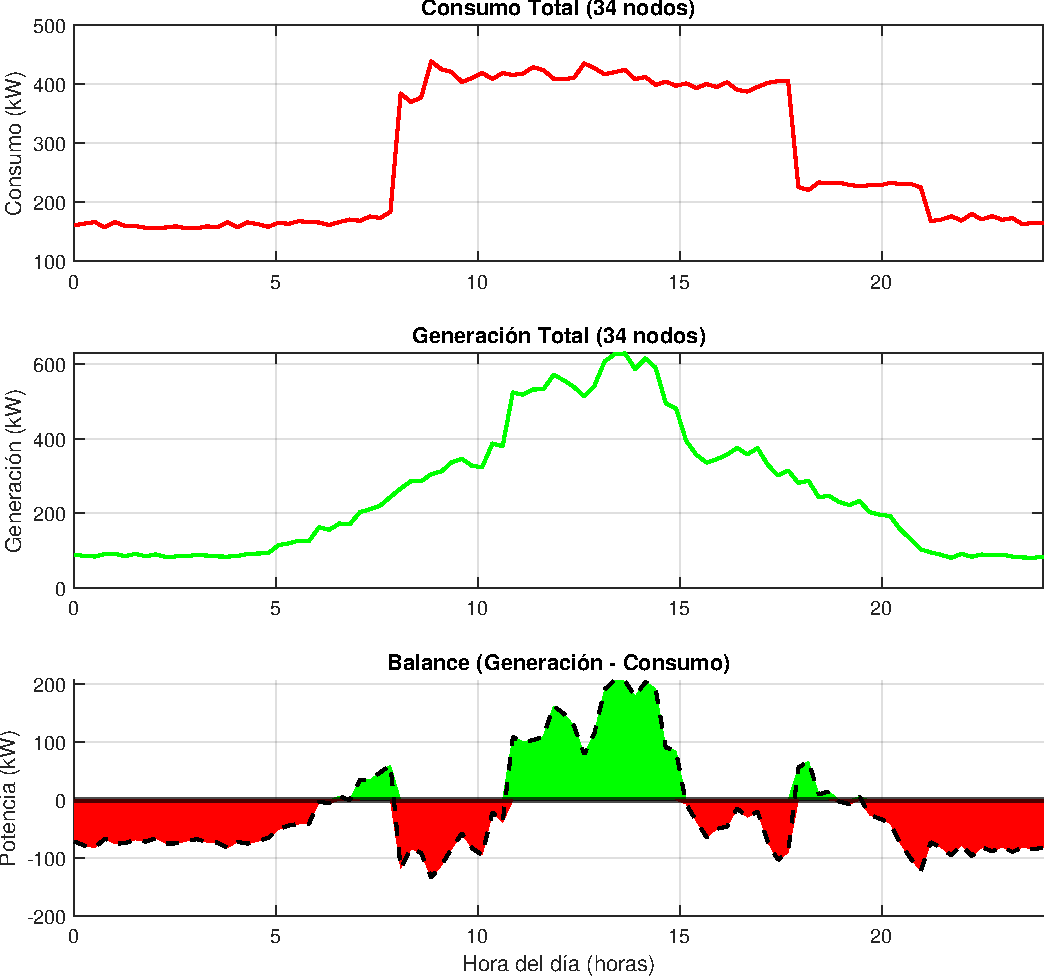
\includegraphics[width=0.6\textwidth]{fig/07_bloste/bloste_17.pdf}
    \caption{Perfiles generales de cargas a lo largo del día empleados con la topología IEEE 34-bus.}
    \label{fig:ieee34_loads}
\end{figure}

Para el modelado de los enlaces de la red se adoptaron igualmente las configuraciones descritas en \cite{Schneider17}, adaptando la distancia física de las líneas a los valores típicos empleados en la topología \gls{ieee} 123-bus. De este modo, se garantiza que tanto las características intrínsecas de las líneas como las pérdidas asociadas resulten comparables en el caso de la topología \gls{ieee} 34-bus. Las configuraciones empleadas se recogen en la Tabla~\ref{tab:links}. La simulación de esta topología se llevó a cabo utilizando la misma jerarquía de clases representada en la Figura~\ref{fig:uml}, así como el mismo entorno de ejecución: un servidor con \textit{Ubuntu 22.04}, equipado con un procesador Intel(R) Core(TM) i9 y 32 GB de memoria RAM. Asimismo, se consideraron los tres escenarios previamente descritos (ideal, con pérdidas, y con pérdidas y restricciones de capacidad en las líneas) junto con los cuatro criterios definidos anteriormente. Como nodo raíz de la topología se seleccionó el nodo 800, obteniéndose las simulaciones únicas que se detallan en la Ecuación~\ref{eq:numsim_bloste_ieee34}.


\begin{equation}\label{eq:numsim_bloste_ieee34}
\begin{aligned}
    \left \langle N_{simulaciones\_ieee34} \right \rangle  \: & = \: N_{deltas} \: \times \: N_{criterios} \: \times \:  N_{escenarios} \: \times \: N_{root}\\ 
    \: & = \: 96 \times 4 \times 3 \times 1\\
    \: & = \: 1152 \: \: simulaciones
\end{aligned}    
\end{equation}
\vspace{0.2cm}


En las Figuras~\ref{fig:v2_fig_base_global_powers} y~\ref{fig:v2_fig_base_global_time_iter} se presentan tanto el balance y el flujo medio de potencia, como el tiempo medio de convergencia y el número medio de iteraciones por criterio. Como se aprecia en la Figura~\ref{fig:v2_fig_base_global_powers}, los resultados de balance y flujo son similares a los obtenidos previamente con la topología de referencia \gls{ieee} 123-bus. En este caso, el criterio \textit{Power2Zero} vuelve a destacar como el de mejor desempeño promedio en el escenario con pérdidas. Sin embargo, al considerar el escenario con pérdidas y restricciones de capacidad en los enlaces, se observa una degradación de este criterio frente a \textit{Hops} y \textit{Low-Link Losses}. Esta diferencia se explica porque, a diferencia de la topología \gls{ieee} 123-bus, que presenta un mayor grado de mallado (\textit{mesh}) y, por tanto, más alternativas de encaminamiento sin alcanzar los umbrales de capacidad, en la topología de 34 nodos las posibilidades de flujo se ven más limitadas. Como consecuencia, en promedio se registran mayores pérdidas, dado que el criterio \textit{Power2Zero}, al basarse en la auto-compensación local entre nodos vecinos, carece de una visión global de la ruta completa. Otro aspecto a destacar es el aumento de los intervalos de confianza. Esto se debe a que el número de muestras por valor medio se ha reducido de 123 a 34 nodos, lo que incrementa la dispersión y la desviación relativa de los resultados. En cuanto a los tiempos de convergencia, representados en la Figura~\ref{fig:v2_fig_base_global_time_iter}, se observa un comportamiento análogo al obtenido con la topología \gls{ieee} 123-bus. No obstante, al tratarse de una red con un menor número de nodos, el tiempo medio de convergencia resulta inferior, alcanzando máximos en torno a los 25 milisegundos, frente a los valores promedio de hasta 45 milisegundos registrados en la topología de 123 nodos.



\begin{figure}[ht!]
    \centering
    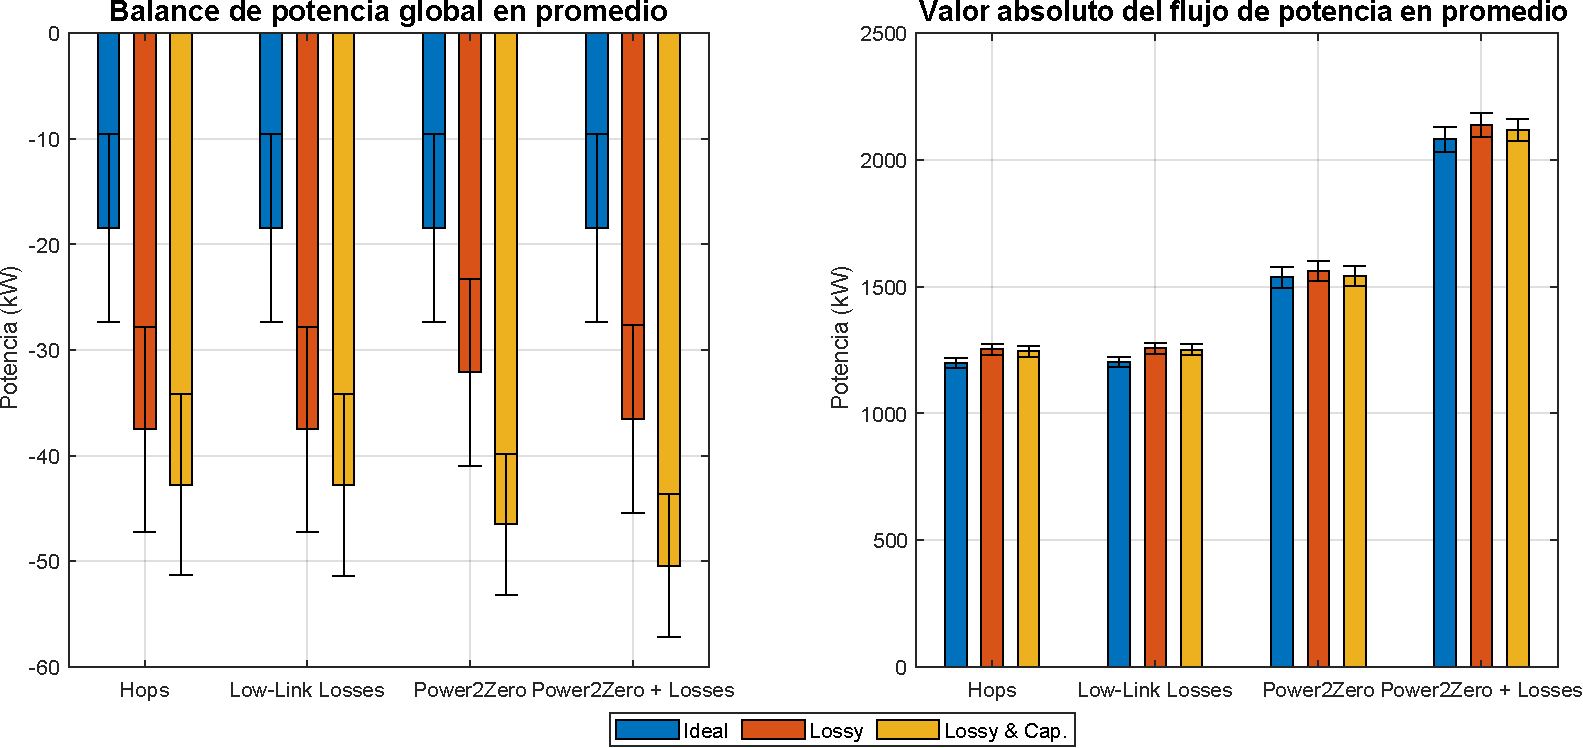
\includegraphics[width=\textwidth]{fig/07_bloste/bloste_18.pdf}
    \caption{Balance de potencia global en promedio y valor absoluto del flujo de potencia - Topología IEEE 34-Node Test Feeder.}
    \label{fig:v2_fig_base_global_powers}
\end{figure}

\begin{figure}[ht!]
    \centering
    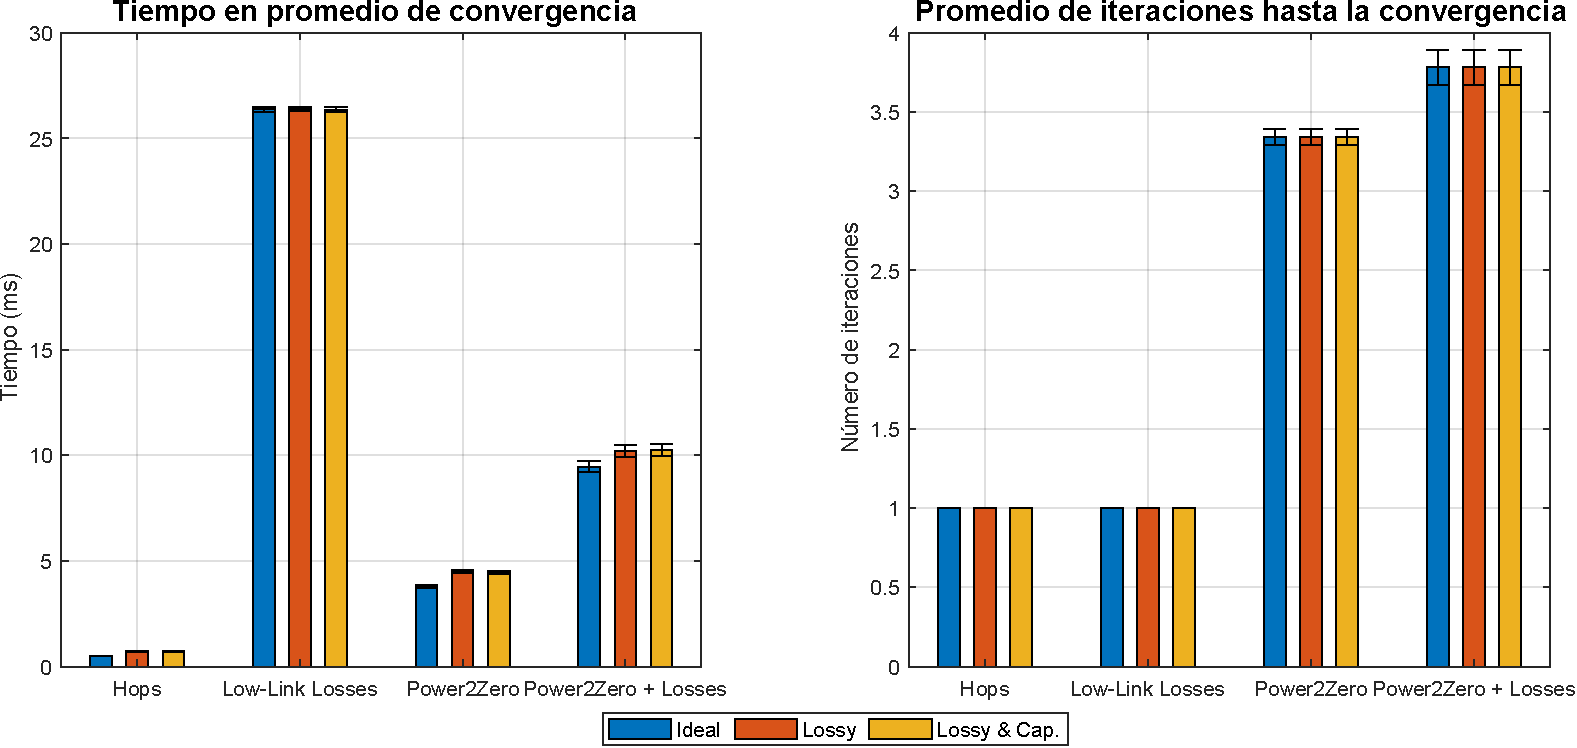
\includegraphics[width=\textwidth]{fig/07_bloste/bloste_19.pdf}
    \caption{Promedio de tiempo/iteraciones hasta la convergencia - Topología IEEE 34-Node Test Feeder.}
    \label{fig:v2_fig_base_global_time_iter}
\end{figure}


\begin{figure}[ht!]
    \centering
    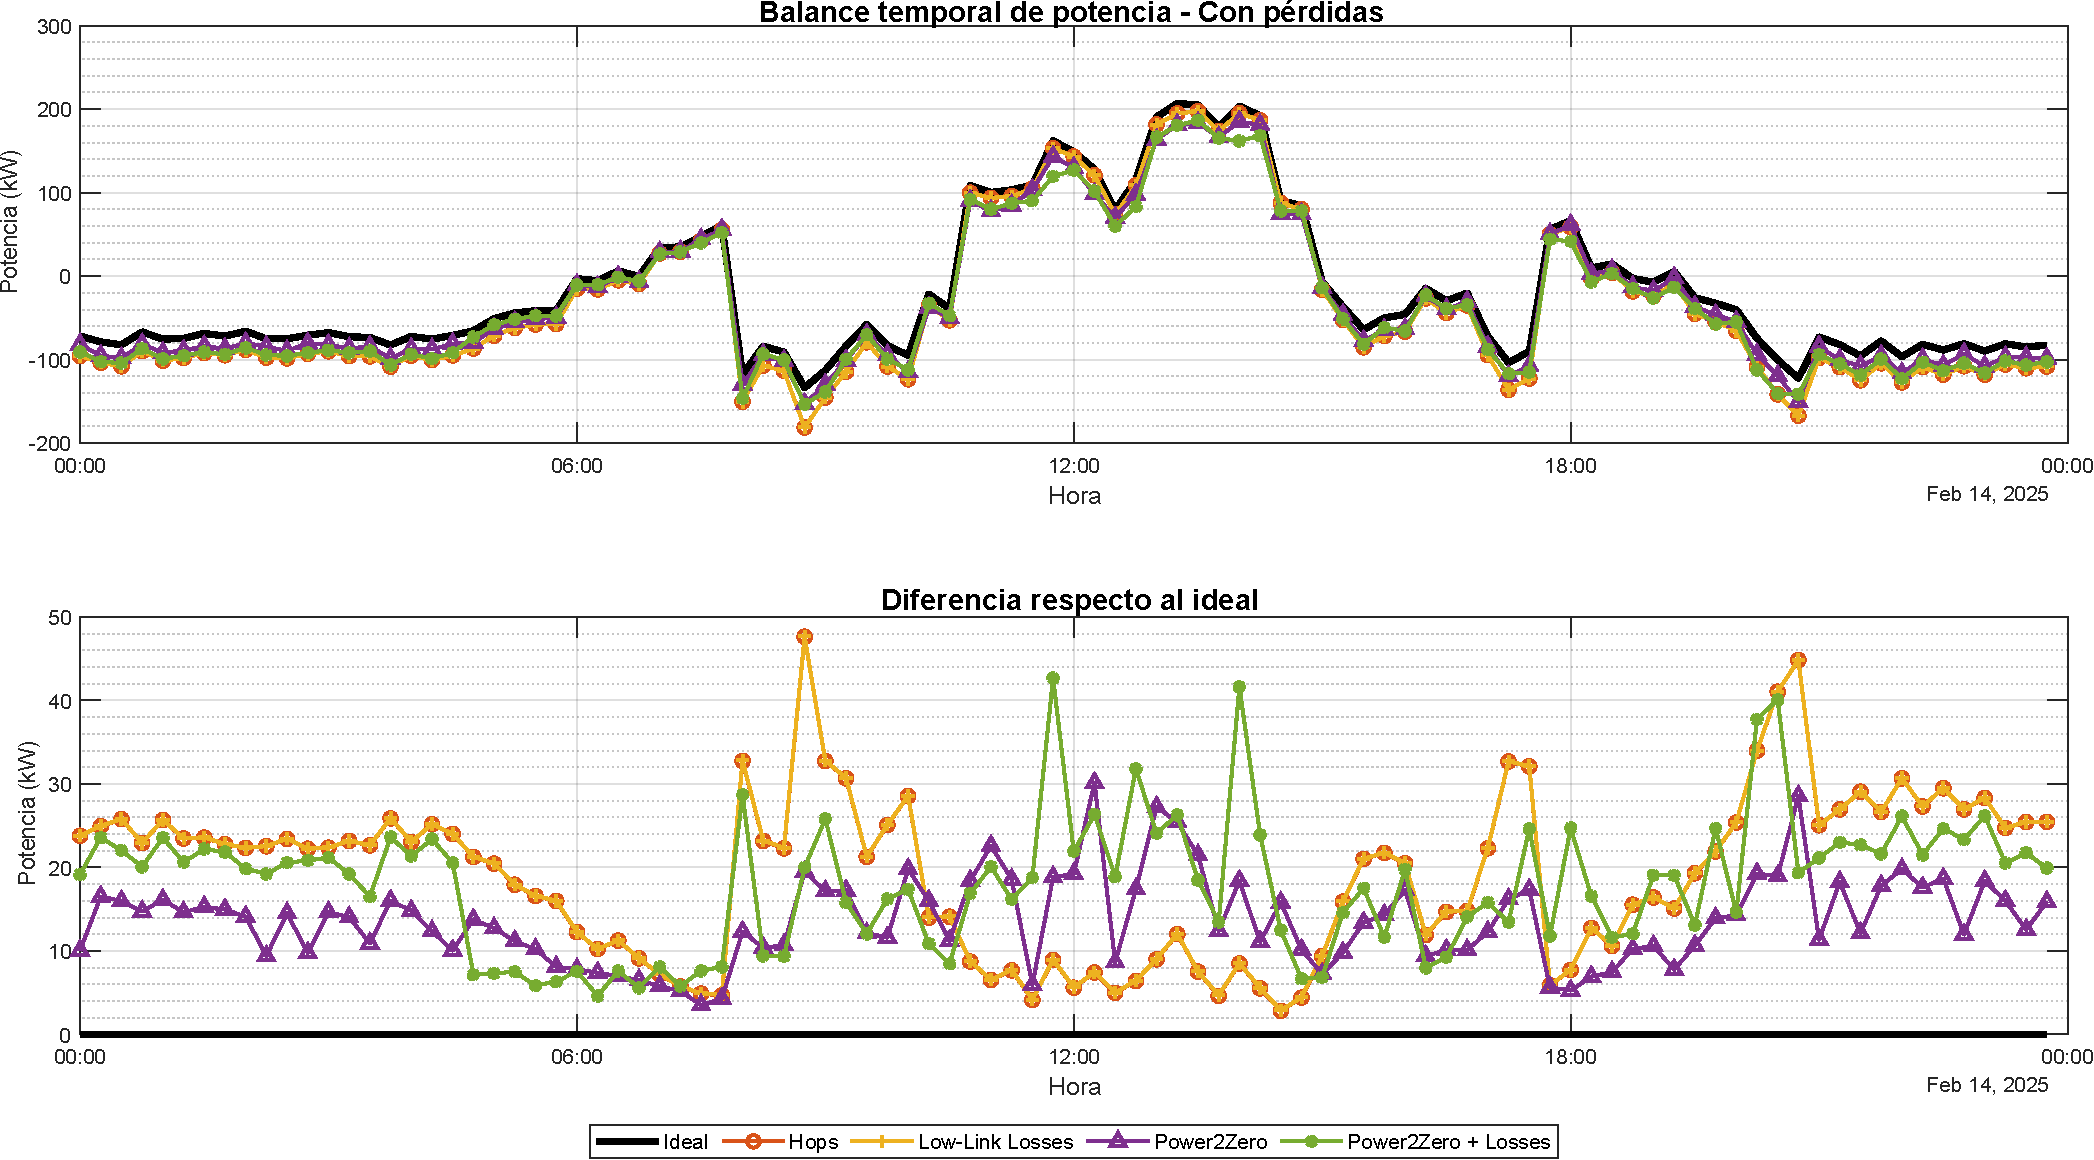
\includegraphics[width=\textwidth]{fig/07_bloste/bloste_20.pdf}
    \caption{Balance temporal de la potencia global en el escenario con pérdidas - Topología IEEE 34-Node Test Feeder.}
    \label{fig:v2_fig_base_TempPowerBalance_Lossy}
\end{figure}

En las Figuras~\ref{fig:v2_fig_base_TempPowerBalance_Lossy} y~\ref{fig:v2_fig_base_TempPowerBalance_LossyCap} se muestra la evolución temporal del balance global de potencia a lo largo de un día completo. Los resultados presentan una fuerte similitud con los obtenidos en la topología de referencia \gls{ieee} 123-bus. Tal como se aprecia, los criterios \textit{Hops} y \textit{Low-Link Losses} exhiben un comportamiento marcadamente homogéneo, al basarse en características intrínsecas de la topología. En contraste, los criterios \textit{Power2Zero} y \textit{Power2Zero + Losses} demuestran una mayor capacidad para optimizar tanto el balance como las pérdidas asociadas, al favorecer la compensación local de demandas y excedentes. En la mayoría de los casos, el criterio \textit{Power2Zero} se confirma como la opción más eficaz. No obstante, en el escenario con pérdidas y restricciones de capacidad en los enlaces se observa una excepción relevante: al existir un menor grado de alternativas para encaminar la potencia, los criterios \textit{Hops} y \textit{Low-Link Losses} alcanzan un mejor desempeño, particularmente durante el periodo valle (08:00–17:30), coincidente con los máximos de generación en la red.


\begin{figure}[ht!]
    \centering
    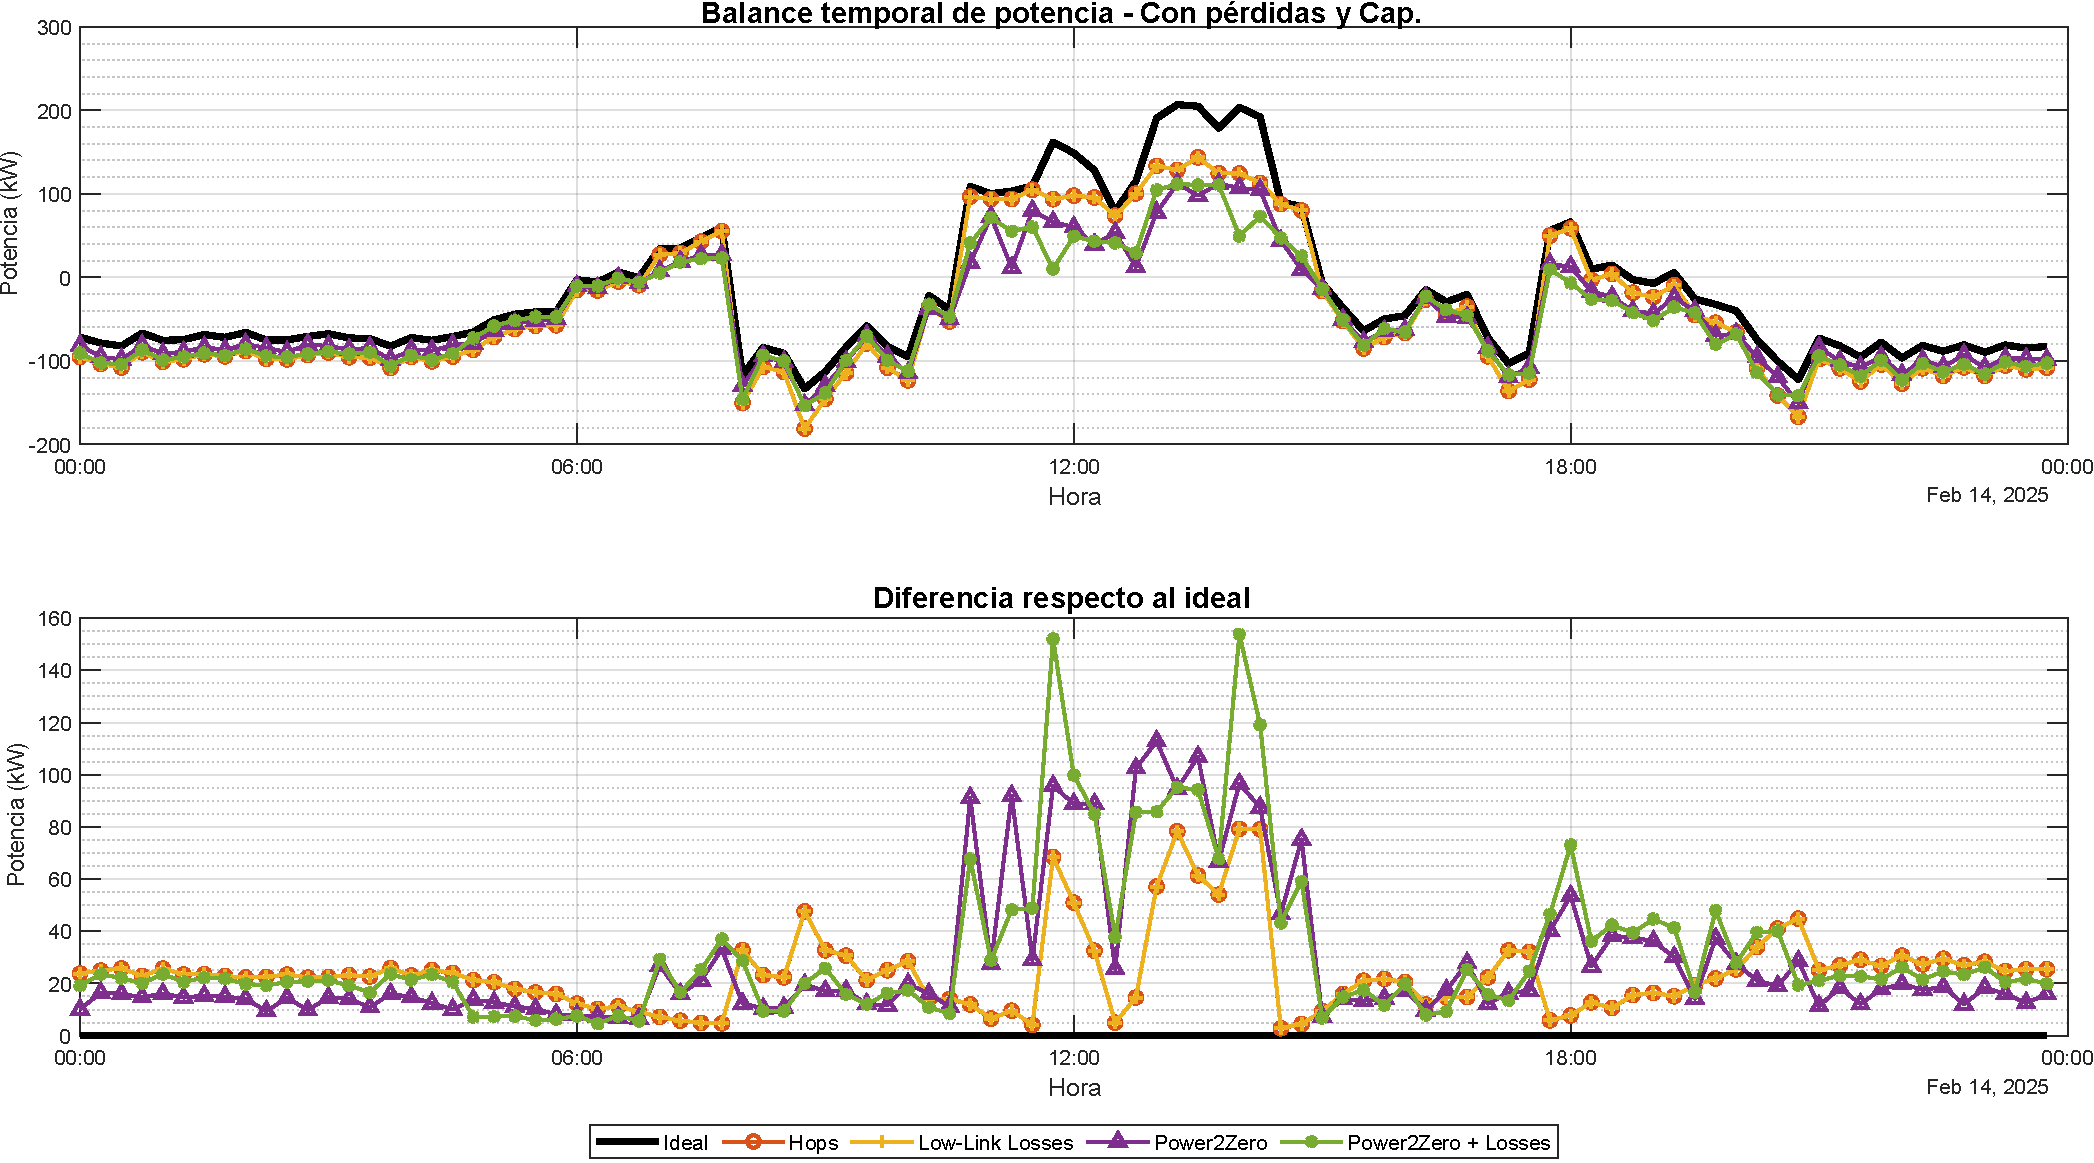
\includegraphics[width=\textwidth]{fig/07_bloste/bloste_21.pdf}
    \caption{Balance temporal de la potencia global en el escenario con pérdidas y capacidades - Topología IEEE 34-Node Test Feeder.}
    \label{fig:v2_fig_base_TempPowerBalance_LossyCap}
\end{figure}


En conjunto, estos resultados evidencian una clara consistencia tanto en el comportamiento de las topologías evaluadas como en el desempeño de los criterios, reforzando así la validez de las conclusiones obtenidas en los distintos escenarios analizados.


\subsection{Estudio de la complejidad computacional}

En esta sección se presenta un análisis de la complejidad computacional del algoritmo. En primer lugar, en la Sección~\ref{subsubsec:ccomplexSpread} se estudia la complejidad asociada al proceso de etiquetado y exploración de la red, mientras que en la Sección~\ref{subsubsec:ccomplexIter} se aborda la complejidad derivada del proceso iterativo y de la aplicabilidad de los criterios diseñados.\\
\\
Para llevar a cabo este estudio, se generaron topologías aleatorias empleando la librería \texttt{NetworkX}\footnote{\url{https://networkx.org/}} de Python, reproduciendo características propias de las topologías de referencia del \gls{ieee}, tales como distancias físicas típicas y configuraciones de enlaces. En lo referente a las cargas, estas fueron generadas aleatoriamente en el rango de $[-4, 4]$ kW a lo largo del día, dado que la configuración de cargas es indiferente para el estudio de la complejidad computacional, pero son necesarias para estudiar el funcionamiento computacional de los criterios. Se consideraron topologías con un número de nodos creciente desde 10 hasta 2500, en incrementos de 10 (\texttt{10:10:2500}), almacenando todas las instancias para garantizar la reproducibilidad de los experimentos. La Figura~\ref{fig:topology_random_70} ilustra un ejemplo de una topología aleatoria generada con 70 nodos. Como puede observarse, las topologías generadas presentan un carácter marcadamente \textit{mesh}, lo que permite poner de manifiesto las ventajas del algoritmo propuesto.

\begin{figure}[ht!]
    \centering
    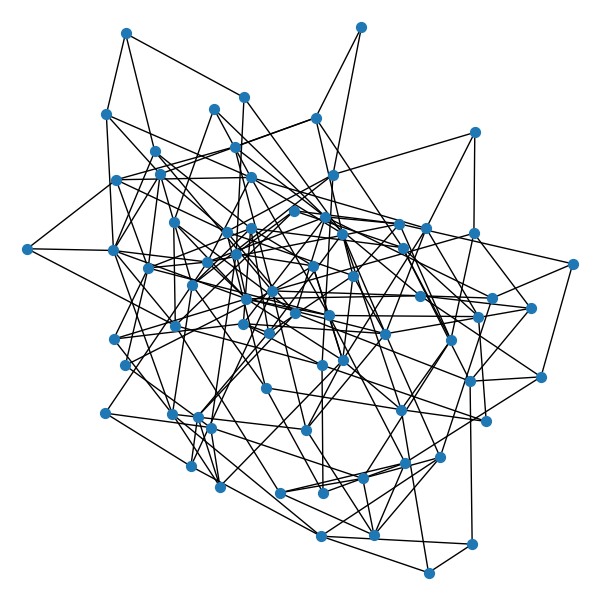
\includegraphics[width=0.5\textwidth]{fig/07_bloste/bloste_22.png}
    \caption{Ejemplo de topología aleatoria generada de 70 nodos para el estudio de la complejidad computacional.}
    \label{fig:topology_random_70}
\end{figure}


\subsubsection{Complejidad computacional del mecanismo de etiquetado del algoritmo}
\label{subsubsec:ccomplexSpread}

Para evaluar la complejidad computacional del proceso de etiquetado (\texttt{spread\_ids}) de nuestro algoritmo, descrito en la Sección~\ref{subsec:tree}, se ha evaluado frente a tres construcciones de árbol alternativas:  \gls{mst}, \gls{pso} y \gls{ga}. Para llevar a cabo la evaluación, se siguió el siguiente protocolo:

\begin{enumerate}
  \item Para cada topología aleatoria de \(n\) nodos (\(n = 10,20,\dots,2500\)):
    
    \begin{itemize}
      
      \item Se cargaron sus ficheros topológicos generados anteriormente con \texttt{NetworkX}.
      
      \item Se eligieron 10 nodos raíz diferentes, al azar, de tal forma: (\(G=(\mathcal{N}, \mathcal{L}) , \mathrm{root}_i\in \mathcal{N}\), \(i=1,\dots,10\)).
      
      \item Para cada nodo raíz, \(\mathrm{root}_i\):
      
        \begin{itemize}
        
          \item Se midió el tiempo de \texttt{spread\_ids}, \(T_{\mathrm{SI}}\).
          
          \item Se midió el tiempo de construcción de un árbol \gls{mst} (usando el algoritmo de Prim~\cite{prim}, implementado en \texttt{NetworkX}), \(T_{\mathrm{MST}}\).
          
          \item Se midió el tiempo de construcción vía \gls{pso} discreto, \(T_{\mathrm{PSO}}\).
          
          \item Se midió el tiempo de construcción vía algoritmo genético, \(T_{\mathrm{GA}}\).
        \end{itemize}
    \end{itemize}
    
  \item Los resultados temporales (\(\{\mathrm{Run},\mathrm{Root},T_{\mathrm{SI}},T_{\mathrm{MST}},T_{\mathrm{PSO}},T_{\mathrm{GA}}\}\)) se almacenaron para su posterior análisis. 

\end{enumerate}

En conjunto, la ejecución completa de las pruebas requirió aproximadamente 50 horas, a continuación, se detallan las implementaciones alternativas, así como los resultados obtenidos.


\paragraph{MST (Prim)} El árbol de descubrimiento mínimo se obtiene con el algoritmo de Prim en un grafo no dirigido \(G=(\mathcal{N}, \mathcal{L})\) ponderado por distancia física de los enlaces \(w_{uv}\). Por tanto:

\begin{equation}
Tree_{\mathrm{MST}} \;=\;\arg\min_{\substack{T\subseteq \mathcal{L}\\|T|=|\mathcal{N}|-1}} 
\sum_{(u,v)\in T} w_{uv}.
\end{equation}

Para orientar el árbol generado hacia el nodo raíz \(\mathrm{root}\), aplicamos un recorrido \gls{bfs} que genera aristas dirigidas \((u\!\to\!v)\) salientes desde la raíz:

\begin{equation}
\mathrm{orient\_tree}(T,\mathrm{root}) = \{(u,v)\in T \mid u \text{ es antecesor de } v \text{ en BFS desde root}\}.
\end{equation}

La complejidad teórica del proceso, se puede estimar como \(O(|\mathcal{L}|\log|\mathcal{N}|)\) para Prim, más \(O(|\mathcal{N}|+|\mathcal{L}|)\) para BFS de orientación. Hay que tener en cuenta que el árbol generado con esta implementación alternativa es una solución que pertenece al subconjunto de arboles generados con nuestro método de de \texttt{spread\_ids}.



\paragraph{PSO discreto} Se diseña un enjambre de \(P\) partículas (En nuestro caso, con 20 partículas), cada una representando un conjunto  de \(|\mathcal{N}|-1\) aristas válidas \(\{e_k\}\subset \mathcal{L}\). Cuya función de \emph{fitness} se define como la suma de las distancias físicas de los enlaces:

\begin{equation}
f(\{e_k\}) = \sum_k w_{e_k}.
\end{equation}

El algoritmo itera \(\ell=1,\dots,L\), siendo $L$ el número de iteraciones totales configurable, y fijado en este caso a 15 iteraciones. Por cada iteración:

\begin{enumerate}
  \item Cada partícula \(p\) del enjambre \(P\):  
    \begin{itemize}
      \item Realiza un cruce de su árbol actual ($\mathrm{p.tree}$), con el mejor árbol de todo el enjambre \(P\) ($\mathrm{gbest.tree}$), de tal forma:  
      \(\mathrm{new} \leftarrow \mathrm{p.tree}\cap \mathrm{gbest.tree}\;\cup\;\text{relleno aleatorio}\).
      \item Se evalúa el nuevo árbol: \(\mathrm{fitness}_p = f(\mathrm{new})\).
      \item Actualización de ($\mathrm{gbest.tree}$) en caso de que haya mejora.
    \end{itemize}
\end{enumerate}

Por tanto, tendremos \(P\) partículas, donde cada partícula  \(p\) representará un árbol. Después de las $L$ iteraciones, se orienta \(\mathrm{gbest.tree}\) igual que en el método de MST, teniendo una complejidad teórica aproximada: \(O(L\,P\,|\mathcal{N}|)\).

\begin{equation}
Tree_{\mathrm{PSO}} = \mathrm{orient\_tree}\bigl(\mathrm{gbest.tree},\,\mathrm{root}\bigr).
\end{equation}


\paragraph{Algoritmo Genético (GA)} Operamos con una población inicial de \(P\) árboles aleatorios, fijada en este caso a 20. Con cada generación \(g\), de $G$ totales fiajadas también a 15, se llevan a cabo los siguientes pasos:

\begin{itemize}
  \item \textbf{Selección}: ordenar por la función de \textit{fitness} (la misma que en el \gls{pso}) \(f(\cdot)\) y seleccionar los \(P/2\) mejores arboles.  
  
  \item \textbf{Cruce}: de cada par de arboles \((T_u,T_v)\) se forma la unión de enlaces 
    \(U = T_u\cup T_v\), y se extrae un \gls{mst} de \(U\) con pesos aleatorios para garantizar 
    \(|\mathcal{N}|-1\) enlaces válidos.  
    
  \item \textbf{Mutación}: con probabilidad \(\mu\) se sustituye aleatoriamente un enlace.  
\end{itemize}

Tras \(G\) generaciones, se toma el mejor el mejor árbol, y se orienta hacia la raíz:

\begin{equation}
Tree_{\mathrm{GA}} = \mathrm{orient\_tree}\bigl(\arg\min_{T\in P}f(T),\,\mathrm{root}\bigr).
\end{equation}

Teniendo una complejidad teórica aproximada de: \(O(G\,P\,|\mathcal{L}|\log|\mathcal{N}|)\), por el \gls{mst} interno en cada cruce.


\paragraph{Resultados} Tras ejecutar la evaluación descrita, se obtuvieron los resultados mostrados en las Figuras~\ref{fig:comparison_4algorithms_linear_spread_ids} y \ref{fig:complexity_comparison_time_spread_ids}, que recogen el análisis de la complejidad computacional de la fase de etiquetado para las cuatro implementaciones consideradas: \gls{blo} (\texttt{spread\_ids}), \gls{mst}, \gls{pso} y \gls{ga}.  

\begin{figure}[ht!]
    \centering
    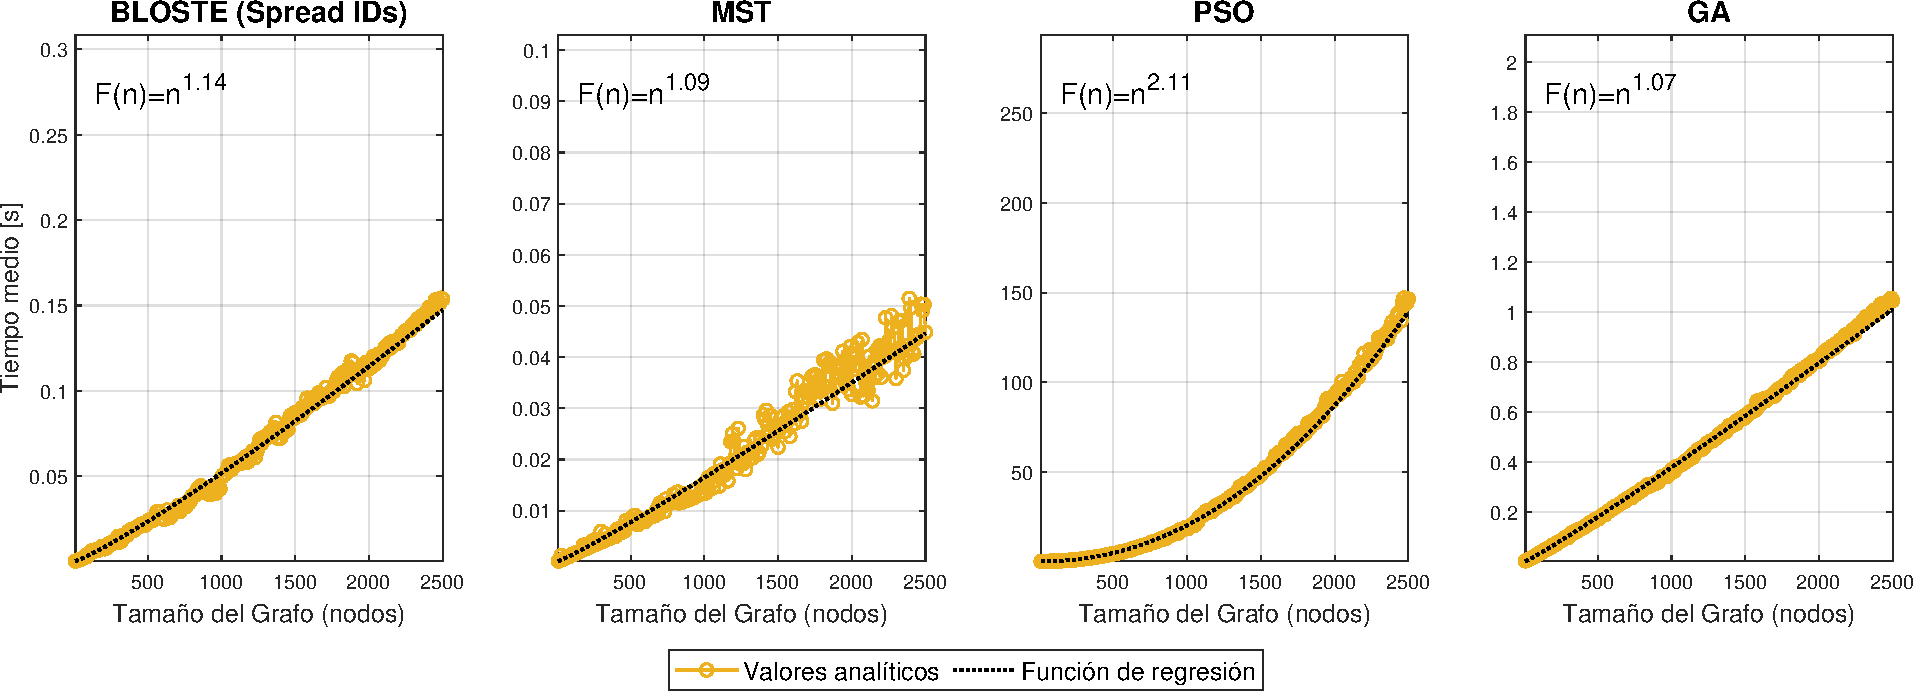
\includegraphics[width=\textwidth]{fig/07_bloste/bloste_23.pdf}
    \caption{Complejidad computacional en la fase de etiquetado.}
    \label{fig:comparison_4algorithms_linear_spread_ids}
\end{figure}

Los resultados de la Figura~\ref{fig:comparison_4algorithms_linear_spread_ids} se obtuvieron promediando todas las ejecuciones de cada algoritmo entre todas las ejecuciones de los diferentes nodos raíz por cada tamaño de grafo, y ajustando los datos mediante regresión lineal con \texttt{polyfit} de \texttt{matlab}. Los valores indican que \gls{blo} escala aproximadamente como \(F(n) = n^{1.14}\), lo que supone un crecimiento casi lineal con una ligera tendencia superlineal. El algoritmo \gls{mst} presenta un ajuste \(F(n) = n^{1.09}\), reflejando un comportamiento prácticamente lineal y una notable eficiencia computacional. El enfoque basado en PSO muestra el mayor coste computacional, con \(F(n) = n^{2.11}\), lo que corresponde a un crecimiento cuadrático con respecto al tamaño del grafo. Por su parte, \gls{ga} presenta \(F(n) = n^{1.07}\), también cercano a lineal, aunque con tiempos absolutos de ejecución superiores a los de \gls{mst} y \gls{blo}. Conviene resaltar que, a diferencia del resto de algoritmos, \gls{blo} genera múltiples árboles en lugar de uno único, característica que, combinada con su baja complejidad, lo convierte en una solución especialmente adecuada en escenarios que requieran redundancia o balanceo de carga, ofreciendo una escalabilidad comparable a la de \gls{mst} y \gls{ga}.  

\begin{figure}[ht!]
    \centering
    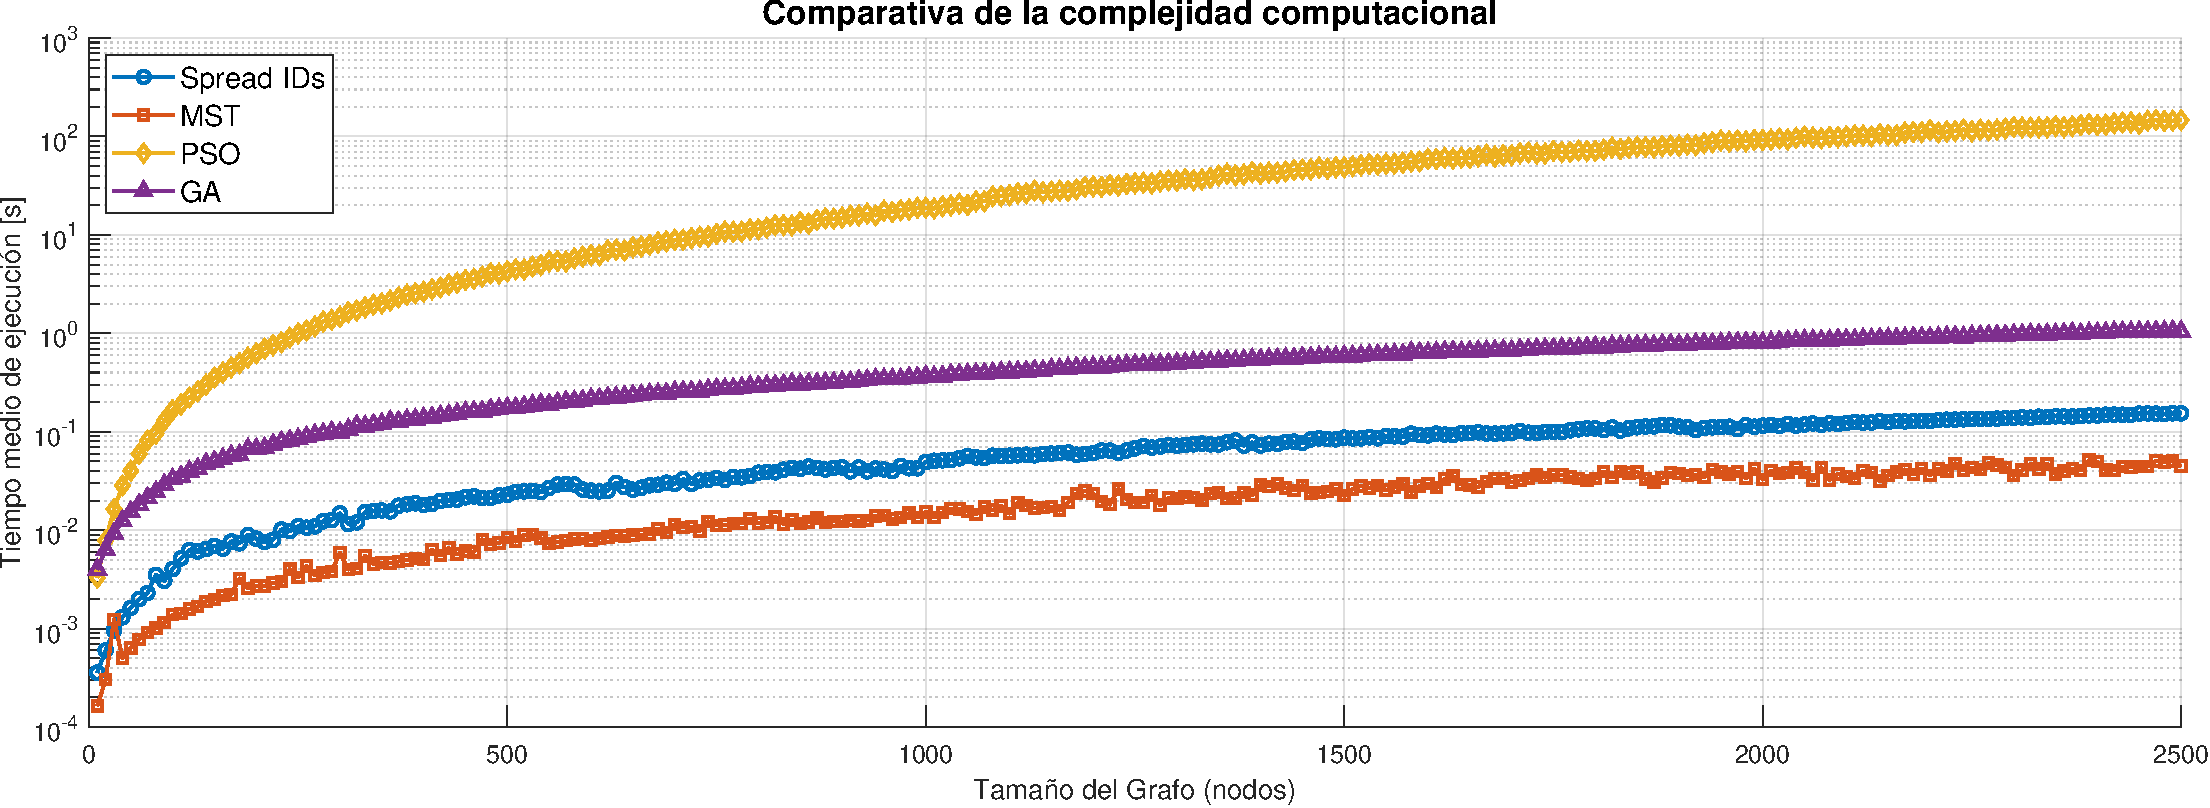
\includegraphics[width=\textwidth]{fig/07_bloste/bloste_24.pdf}
    \caption{Comparativa de la complejidad computacional en tiempo con escala logarítmica.}
    \label{fig:complexity_comparison_time_spread_ids}
\end{figure}

La representación en escala logarítmica de la Figura~\ref{fig:complexity_comparison_time_spread_ids} confirma estas tendencias: las pendientes casi paralelas de \gls{blo}, \gls{mst} y \gls{ga} reflejan complejidades empíricas similares, mientras que \gls{pso} exhibe una pendiente significativamente más pronunciada. Además, \gls{blo} mantiene una ventaja constante sobre \gls{ga} y \gls{pso} en tiempo absoluto de ejecución para todos los tamaños de grafo evaluados. Aunque sus tiempos son superiores a los de \gls{mst}, el hecho de generar múltiples árboles simultáneamente lo convierte en una alternativa muy atractiva en redes supermalladas, ya que proporciona mayor flexibilidad y capacidad de adaptación en el encaminamiento de recursos energéticos.


\subsubsection{Complejidad computacional del mecanismo iterativo del algoritmo}
\label{subsubsec:ccomplexIter}

Tal y como se introdujo en la Sección~\ref{subsec:iterativeBalance}, \gls{blo} incorpora un mecanismo iterativo destinado a refinar progresivamente la configuración de la red de acuerdo con unos criterios de decisión predefinidos, con el objetivo de alcanzar un balance de potencia adecuado en la red de distribución eléctrica. Para estimar la complejidad computacional de dicho mecanismo, se emplearon las topologías aleatorias previamente generadas, junto con perfiles de carga definidos en el rango \([-4,4]\) kW. Aunque estos perfiles carecen de validez práctica desde el punto de vista eléctrico, resultan útiles para analizar el comportamiento computacional de los criterios. En este caso no se han considerado algoritmos alternativos con los que establecer comparaciones, dado que la naturaleza configurable de los criterios hace que su implementación dependa del caso de uso final. Por ello, el estudio se centró exclusivamente en el rendimiento y la complejidad computacional de los cuatro criterios presentados.  Para llevar a cabo la evaluación, se siguió el siguiente protocolo:


\begin{enumerate}
  \item Para cada topología aleatoria de \(n\) nodos (\(n = 10,20,\dots,2500\)):
    
    \begin{itemize}
      
      \item Se cargaron sus ficheros topológicos generados anteriormente con \texttt{NetworkX}.
      
      \item Se eligieron 10 nodos raíz diferentes, al azar, de tal forma: (\(G=(\mathcal{N}, \mathcal{L}) , \mathrm{root}_i\in \mathcal{N}\), \(i=1,\dots,10\)).
      
      \item Para cada nodo raíz, \(\mathrm{root}_i\):
      
        \begin{itemize}
          \item Se cargan los 96 $\delta$ de cargas en cada nodo de la topología (representando cada $\delta$ un intervalo de 15 minutos), por cada $\delta_{carga}$:

          \begin{itemize}

              \item Se midió el tiempo por cada criterio $(T_{\mathrm{c1}},T_{\mathrm{c2}},T_{\mathrm{c3}},T_{\mathrm{c4}})$, hasta que no hubiera cargas encerradas en la topología, es decir, que convergiera el método iterativo. 
           \end{itemize}
        \end{itemize}
    \end{itemize}
    
  \item Los resultados temporales (\(\{\mathrm{Run},\mathrm{Root},\delta_{carga},T_{\mathrm{c1}},T_{\mathrm{c2}},T_{\mathrm{c3}},T_{\mathrm{c4}}\}\)) se almacenaron para su posterior análisis. 

\end{enumerate}

En conjunto, la ejecución completa de las pruebas requirió aproximadamente 60 horas, cuyos resultados se presentan y discuten a continuación.

\paragraph{Resultados} En esta sección se presentan los resultados del estudio de la complejidad computacional del proceso iterativo, evaluado bajo los distintos criterios descritos previamente. Para cada topología se seleccionaron diez raíces con semilla fija y, para cada raíz, se consideraron los 96 intervalos temporales correspondientes a un día completo. Con el fin de obtener una medida representativa por topología y criterio, se aplicó un esquema de doble promedio: en primer lugar, se calcularon los tiempos medios sobre las 96 deltas temporales de cada raíz; posteriormente, estos promedios se agregaron entre las diez raíces, obteniéndose así un valor final por criterio y topología.\\
\\
Las Figuras~\ref{fig:iterative_regressions_4criteria} y~\ref{fig:iterative_complexity_double_average} muestran, respectivamente, (i) el ajuste de regresión obtenido mediante la función \texttt{polyfit} para cada criterio, y (ii) la comparación de los tiempos medios (doble promedio) en función del tamaño de la topología. A partir de la representación en escala \(\log\!-\!\log\), se aproximó la dependencia temporal mediante una ley de potencia de la forma

\begin{equation}
    T(n) \approx C \, n^{\gamma},
\end{equation}

donde \(n\) representa el número de nodos de la topología, \(C\) es una constante de escala y \(\gamma\) el exponente estimado mediante ajuste lineal de \(\log T\) frente a \(\log n\). Los valores obtenidos para cada criterio son los siguientes:

\begin{equation}
\begin{aligned}
    \text{Hops:} \quad & T_{\mathrm{Hops}}(n) \approx C_{\mathrm{H}} \, n^{1.32}\\
    \text{Low-Link Losses:} \quad & T_{\mathrm{LLL}}(n) \approx C_{\mathrm{LL}} \, n^{1.17}\\
    \text{Power2Zero:} \quad & T_{\mathrm{P2Z}}(n) \approx C_{\mathrm{P2Z}} \, n^{1.36}\\
    \text{Power2Zero+Losses:} \quad & T_{\mathrm{P2Z+L}}(n) \approx C_{\mathrm{P2ZL}} \, n^{1.34}
\end{aligned}
\end{equation}

\begin{figure}[ht!]
    \centering
    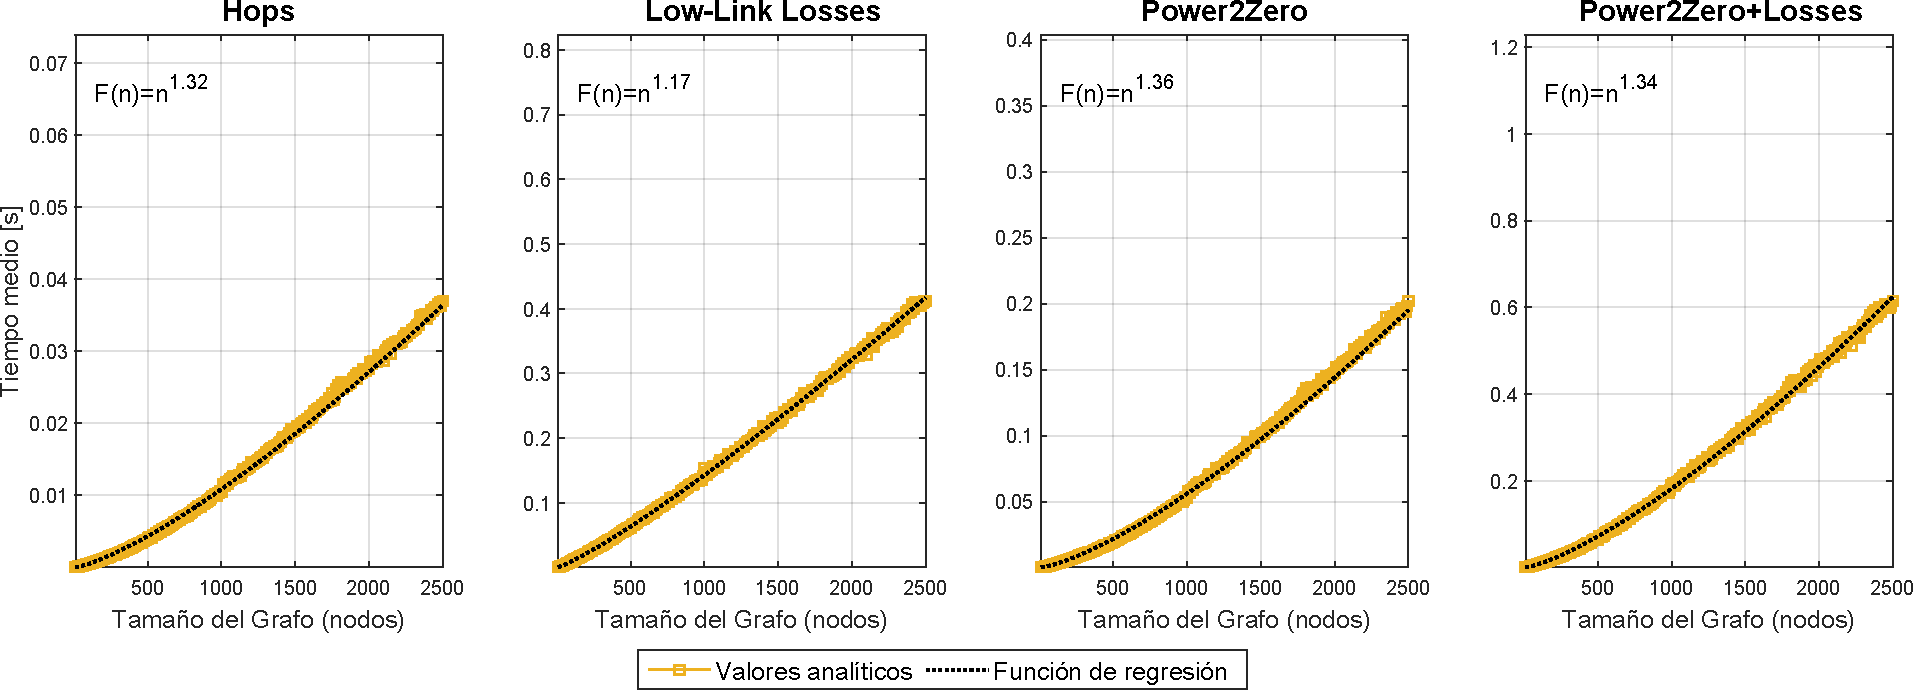
\includegraphics[width=\textwidth]{fig/07_bloste/bloste_25.pdf}
    \caption{Complejidad computacional del mecanismo iterativo.}
    \label{fig:iterative_regressions_4criteria}
\end{figure}

Estos resultados se representan gráficamente en la Figura~\ref{fig:iterative_regressions_4criteria}, donde se indican las leyes de potencia ajustadas para cada criterio. El análisis permite extraer varias observaciones relevantes. En primer lugar, todos los exponentes \(\gamma\) se encuentran en el rango aproximado \(1.17\!-\!1.36\), lo que refleja un crecimiento ligeramente superlineal del tiempo de ejecución con respecto al tamaño de la topología. En la práctica, esto implica que duplicar el número de nodos incrementa el tiempo de ejecución en algo más del doble, aunque lejos de un comportamiento cuadrático.\\
\\
En segundo lugar, se aprecian diferencias entre los criterios: el enfoque \textit{Low-Link Losses} presenta el menor exponente (1.17), lo que sugiere un crecimiento más moderado en comparación con el resto, mientras que \textit{Power2Zero} y \textit{Power2Zero+Losses} alcanzan exponentes ligeramente superiores (1.34–1.36), sin embargo, la base de tiempos es significativamente menor para \textit{Power2Zero}, y para \textit{Power2Zero+Losses} es similar, debido a que requiere más iteraciones para converger en la topología. La Figura~\ref{fig:iterative_complexity_double_average} ilustra los tiempos medios absolutos (doble promedio), donde se observa, además, un cruce característico entre el criterio de bajas pérdidas y el de \textit{Power2Zero+Losses}. Este comportamiento se explica porque, a medida que aumenta el tamaño del grafo, el criterio de bajas pérdidas debe evaluar un mayor número de identificadores y vecinos, lo que incrementa gradualmente su coste computacional. \\
\\
Finalmente, cabe destacar que, incluso en topologías de hasta 2500 nodos, los tiempos medios por criterio permanecen dentro de escalas reducidas, del orden de décimas a fracciones de segundo, lo que demuestra que el mecanismo iterativo, en su implementación actual, resulta computacionalmente viable para las dimensiones de red consideradas.



\begin{figure}[ht!]
    \centering
    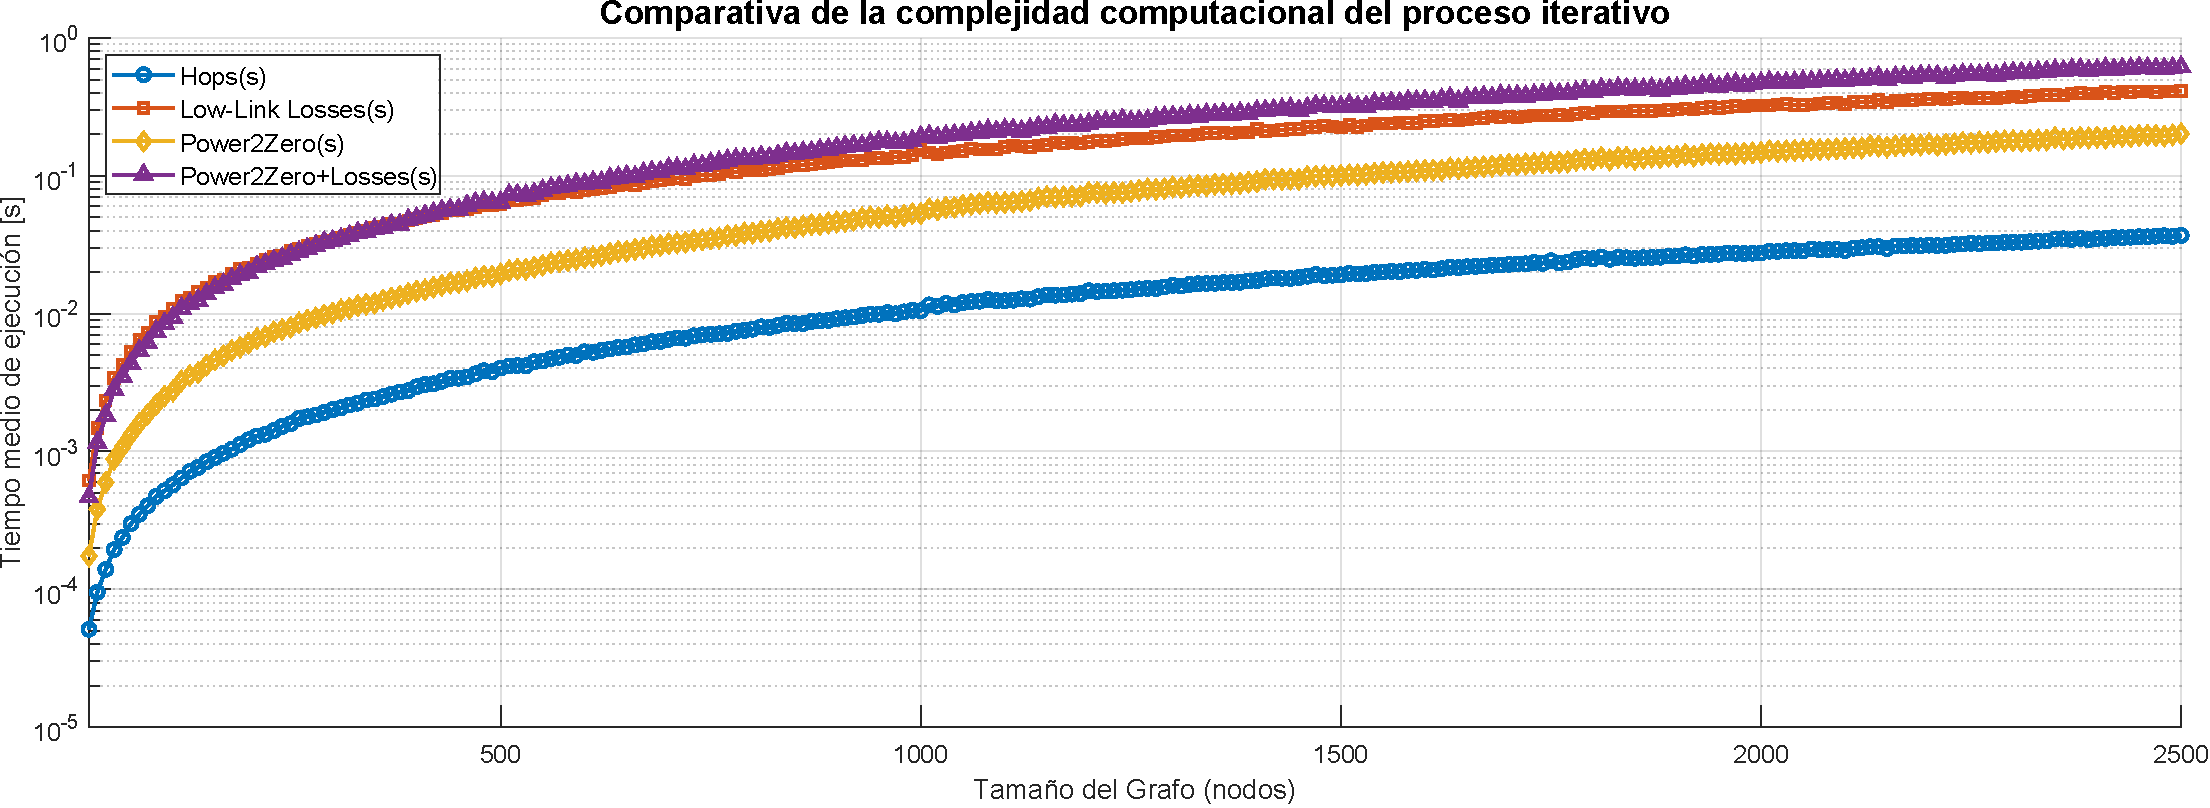
\includegraphics[width=\textwidth]{fig/07_bloste/bloste_26.pdf}
    \caption{Comparativa de la complejidad computacional del mecanismo iterativo en tiempo con escala logarítmica.}
    \label{fig:iterative_complexity_double_average}
\end{figure}

\section{Conclusiones}

En este trabajo se ha presentado \gls{blo}, un algoritmo que permite el encaminamiento adaptativo y en tiempo real de energía en redes de distribución malladas. \gls{blo} aborda las principales limitaciones de los sistemas centralizados mediante el uso de superposiciones lógicas (\textit{overlays}) iniciadas desde uno o varios nodos raíz, en combinación con estrategias de optimización multicriterio flexibles. Estas características confieren al sistema capacidad de operar bajo condiciones variables y con distintos objetivos de control, promoviendo así la escalabilidad, la capacidad de respuesta y la resiliencia del sistema.\\
\\
La evaluación realizada sobre la topología de referencia \gls{ieee} 123-bus en tres escenarios (ideal, con pérdidas y con pérdidas y restricciones de capacidad en los enlaces), con más de 148\,000 simulaciones, ha permitido llevar a cabo un análisis exhaustivo de los criterios de encaminamiento propuestos. Cada escenario incluyó 96 configuraciones de carga distintas y múltiples emplazamientos del nodo raíz, lo que permitió una comparación detallada. Entre los criterios evaluados, el criterio local \textit{Power2Zero} se consolidó como la mejor opción en términos de balance global de potencia, alcanzando un desequilibrio medio de $-4.1\%$ en promedio entre los diferentes nodos raíz. Aunque no es el criterio más rápido en términos de convergencia (4.02 ms frente a 1.40 ms del criterio de \textit{Hop}), este compromiso queda compensado por su superior capacidad de balanceo. Además, pese a requerir aproximadamente el doble de iteraciones, la relación entre el tiempo de convergencia y el número de iteraciones se mantuvo en niveles de eficiencia similares, lo que confirma su viabilidad práctica en escenarios de operación en tiempo real.\\
\\
Los resultados obtenidos se han validado adicionalmente en la topología \gls{ieee} 34-bus, bajo las mismas condiciones de evaluación. Los patrones observados en la topología de mayor tamaño se reprodujeron de manera consistente, confirmando la solidez del comportamiento de los criterios bajo distintas estructuras de red. En particular, se observó que, en topologías con menor grado de mallado, los criterios de \textit{Hop} y \textit{Low-Link Losses} tienden a ofrecer un desempeño más competitivo en escenarios con restricciones de capacidad, mientras que \textit{Power2Zero} mantiene su superioridad en escenarios menos restringidos. Esta consistencia entre topologías refuerza la generalidad y robustez de los resultados obtenidos.\\
\\
Adicionalmente, se ha llevado a cabo un estudio detallado de la complejidad computacional del algoritmo, abarcando tanto el mecanismo de etiquetado como el proceso iterativo. Los análisis muestran que la fase de etiquetado (\texttt{spread\_ids}) escala de forma prácticamente lineal, con un comportamiento comparable al de algoritmos clásicos como \gls{mst} o \gls{ga}, pero con la ventaja de generar múltiples árboles en lugar de uno único. Por su parte, el mecanismo iterativo presenta un crecimiento ligeramente superlineal en todos los criterios, con exponentes en el rango $1.17\!-\!1.36$, lo que garantiza tiempos de ejecución de apenas décimas a fracciones de segundo incluso para topologías de hasta 2500 nodos. Estos resultados demuestran que \gls{blo} no solo es efectivo desde el punto de vista del balance de potencia, sino también computacionalmente viable y escalable para redes de distribución de gran tamaño.\\
\\
Finalmente, cabe destacar la relevancia de disponer de \textit{datasets} de microredes para la mejora continua tanto de los mecanismos de predicción como de los criterios de selección. La disponibilidad de topologías más diversas y de conjuntos de datos abiertos contribuiría significativamente al entrenamiento y refinamiento del sistema. Aunque este estudio ha incorporado un grado considerable de heterogeneidad mediante la evaluación de las topologías \gls{ieee} 123-bus y \gls{ieee} 34-bus, así como mediante topologías aleatorias de gran escala, resultará necesario ampliar las pruebas a escenarios de red más variados y complejos. Dado que los criterios de decisión son configurables, futuras investigaciones deberían explorar cómo la parametrización de los mismos afecta al rendimiento en distintos tipos de redes, consolidando así la aplicabilidad de \gls{blo} como una herramienta versátil y robusta para la gestión energética en redes de distribución malladas.